\documentclass[acmsmall,screen,anonymous,review]{acmart}
\settopmatter{printfolios=true,printccs=false,printacmref=false}

%% Journal information
%% Supplied to authors by publisher for camera-ready submission;
%% use defaults for review submission.
\acmJournal{PACMPL}
\acmVolume{1}
\acmNumber{CONF} % CONF = POPL or ICFP or OOPSLA
\acmArticle{1}
\acmYear{2018}
\acmMonth{1}
\acmDOI{} % \acmDOI{10.1145/nnnnnnn.nnnnnnn}
\startPage{1}

\setcopyright{none}

\bibliographystyle{ACM-Reference-Format}
\citestyle{acmauthoryear}   %% For author/year citations

%%%%%%%%%%%%%%%%%%%%%%%%%%%%%%%%%%%%%%%%%%%%%%%%%%%%%%%%%%%%

%  \citestyle{acmauthoryear}
\usepackage{ amssymb }
\usepackage{stmaryrd}


\usepackage{subcaption}
\usepackage[T1]{fontenc}
\usepackage[utf8]{inputenc}
\usepackage[british]{babel}
\usepackage{xspace, listings, lstcustom, wrapfig, graphicx, enumerate}
\usepackage{paralist}
\usepackage{color,colortbl, relsize}
\usepackage{rotating}
\usepackage{pifont}
\usepackage{multirow}
\usepackage{soul}
\usepackage{tcolorbox}
\usepackage[scaled=.9, light]{zlmtt}
\usepackage{siunitx}
\usepackage{setspace}

 \newcommand{\ttt}{\prg{true}}
\newcommand{\ff}{\prg{false}}
\newcommand{\unkn}{\prg{b???}}
\newcommand{\bv}{\prg{bval}}

\newcommand{\sdparagraph}[1]{{\vspace{.3cm} \noindent \textit{#1}\ }}

\newcommand{\prg}[1]{{\mbox{\tt{#1}}}}

\newcommand{\m}{\prg{m}}
 \newcommand{\f}{\prg{f}}
  \newcommand{\e}{\prg{e}}
 \renewcommand{\c}{\prg{C}}
 \renewcommand{\v}{\prg{v}}
  \newcommand{\x}{\prg{x}}
  \newcommand{\p}{\prg{p}}
   \newcommand{\y}{\prg{y}}
      \newcommand{\uu}{\prg{u}}
  %  \newcommand{\z}{\prg{z}}
  \newcommand{\this}{\prg{this}}
  \newcommand{\caller}{\kw{caller}}
   \newcommand{\nullK}{\prg{null}}
\newcommand{\addr}{\ensuremath{\alpha}}


\newcommand{\fldMap}{\textit{fldMap}}

\newcommand{\forget}[1]{}
\newcommand{\etc}{{\it etc.}}
\newcommand{\eg}{{\it e.g.\,}}
\newcommand{\ie}{{\it i.e.\,}}

% new macros for holistic
\newcommand{\Future}[1] {\ensuremath{{\mathsf{will}}\langle \,#1\,\rangle}}
\newcommand{\Using}[2]{\ensuremath{\langle\, #1\, \mathsf{in}\, #2\, \rangle}}
\newcommand{\External}[1] {\ensuremath{{\mathsf{external}}\langle\,  #1\, \rangle}}
\newcommand{\Internal}[1] {\ensuremath{{\mathsf{internal}}\langle\,  #1\, \rangle}}
\newcommand{\Changes}[1]{\ensuremath{{\mathsf{changes}}\langle\,#1\,\rangle}}
\newcommand{\CanAccessTr}[2]{\ensuremath{\langle\, #1\, \mathsf{access}^*\, #2\, \rangle}}
\newcommand{\CanAccess}[2]{\ensuremath{\langle\, #1\, \mathsf{access}\, #2\, \rangle}}

\newcommand{\Calls}[4]{\ensuremath{\langle\, #1\, \mathsf{calls}\, #3.#2\lp#4\rp\, \rangle}}%(\!({#1})\!)}
\newcommand{\Next}[1] {\ensuremath{{\mathsf{next}}\langle \,#1\,\rangle}}%(\!({#1})\!)}
\newcommand{\PrevId}{\ensuremath{{\mathcal{P}}\textrm{\textit{rev}}}}
\newcommand{\Prev}[1] {\ensuremath{{\mathsf{prev}}\langle \,#1\,\rangle}}%(\!({#1})\!)}
\newcommand{\Past}[1]  {\ensuremath{{\mathsf{was}}\langle \,#1\,\rangle}}

\newcommand{\Name}[2]  {\ensuremath{{\mathsf{name}}\langle \,#1, #2\rangle}}

% old macros for holistic
%\newcommand{\Future}[1] 
%{{{\mathcal W}\!ill}\langle#1\rangle}%{\lozenge\, #1}% {\bullet #1}% {{{\mathcal F}}(#1)} % {{{\mathcal B}}(#1)}
%\newcommand{\Using}[2]{{\mathcal W}ith\langle\ #2,\,#1\ \rangle}
% \newcommand{\External}[1]{{\mathcal E}xternal\langle #1\rangle}
%\newcommand{\Using}[2]{#1\,{\mathcal U}sing\, #2}
%\newcommand{\Using}[2]{#1\,{\mathcal U}sing\, #2} %{{{\mathcal U}}(#1,#2)}
% \newcommand{\Changes}[1]{\ensuremath{\mathcal{C}\textrm{\textit{hange}}\langle#1\rangle}}
%\newcommand{\CanAccessTr}[2]{\ensuremath{\mathcal{A}}\textrm{\textit{ccess}}^*\langle #1,#2\rangle}
%\newcommand{\CanAccess}[2]{\ensuremath{{\mathcal{A}}\textrm{\textit{ccess}}}\langle #1,#2\rangle}%(#1,#2)}
%\newcommand{\Calls}[4]{\ensuremath{{\mathcal{C}}\textrm{\textit{alls}}}\langle #1,#2,#3,#4\rangle}%(\!({#1})\!)}
%\newcommand{\Next}[1]{\ensuremath{{\mathcal{N}}\textrm{\textit{ext}}}\langle #1\rangle}%(\!({#1})\!)}
%\newcommand{\PrevId}{\ensuremath{{\mathcal{P}}\textrm{\textit{rev}}}}
%\newcommand{\Prev}[1]{\ensuremath{{\mathcal{P}}\textrm{\textit{rev}}}\langle #1\rangle}%(\!({#1})\!)}
%\newcommand{\Caller}{\ensuremath{{\mathcal{C}}\textrm{\textit{aller}}}}

%\newcommand{\VisibleLit}{\ensuremath{\mathcal{V}\textrm{\textit{isible}}}}
%\newcommand{\Next}[1]{\ensuremath{{\mathcal{N}}\textrm{\textit{ext}}}\langle #1\rangle}%(\!({#1})\!)}
%\newcommand{\PrevId}{\ensuremath{{\mathcal{P}}\textrm{\textit{rev}}}}
%\newcommand{\Prev}[1]{\ensuremath{{\mathcal{P}}\textrm{\textit{rev}}}\langle #1\rangle}%(\!({#1})\!)}
%\newcommand{\Caller}{\ensuremath{{\mathcal{C}}\textrm{\textit{aller}}}}
% \newcommand{\Past}[1] {{{\mathcal W}\!as}\langle#1\rangle}% {\nabla #1} %{\lozenge\!\!\!\!\-\!\!-\,#1}


\newcommand{\SigmaUsing}[2]{#1\@ #2} %{{{\mathcal U}}(#1,#2)}
%{\lozenge\!\!\!\!\!\circ  #1} % {\lozenge\!\!\!\!\-\!\!- #1} %{\upupsilon #1}  %{\nabla #1} %{\circ #1}%  {{{\mathcal P}}(#1)}
\newcommand{\Initial}[1] {{{\mathcal I}\!nitial}\langle#1\rangle}

\newcommand{\Pol}[1] {{\ensuremath{\prg{Pol}\_{\prg{#1}}}}}

\newcommand{\strongImplies}{\leqq} %{{ \,^\sqsubset\!\!\!_{\sim}\, }}
\newcommand{\weakImplies}{\lessapprox} %{{ \,^\sqsubset\!\!\!_{\sim}\, }}
\newcommand{\frames}{~\kw{frames}~}

\newcommand{\appref}[1]{see App.~\ref{#1}}

\newcommand{\sE}{{\prg{e}}}
\newcommand{\varMap}{{\ensuremath{\beta}}}

\newcommand{\Lang} {\ensuremath{{\mathcal L}{_1}}}
\newcommand{\LangOO} {\ensuremath{{\mathcal L}{_{\tt {oo}}}}\xspace}
\newcommand{\Chainmail} {\ensuremath{{\mathcal C}hainmail}\xspace}

% ------------------------------------------------------------------
%                                             positions, separations
\newcommand{\cf}{{\it c.f.~}}
\newcommand{\HYPHENA}{{\em-- }}
\newcommand{\HYPHENB}{{\em-- }}
\newcommand{\SP}{{\hspace{.1in}}}
\newcommand{\s}{{\hspace{.01in}}}

\newcommand{\obeys}{\,\textbf{\textrm{obeys}}\,}
\newcommand{\StrongDom}{\ensuremath{\mathcal{S}\textrm{\textit{trong}}{\mathcal{D}}\textrm{\textit{om}}}}
\newcommand{\Dom}{\ensuremath{\mathcal{D}}\textrm{\textit{om}}}


\newcommand{\Gives}{\ensuremath{\mathcal{G}\textrm{\textit{ives}}}}
%{\ensuremath{\mathcal{C}\textrm{\textit{an}}{\mathcal{A}}\textrm{\textit{ccess}}}(#1,#2)}
\newcommand{\A}{\ensuremath{A}}
\newcommand{\B}{\ensuremath{B}}
\newcommand{\Arising}[1]{{\mathcal{A}}\textrm{\textit{rising}}(#1)}

 %------------------------ syntax tables

\newcommand{\syntax}[1]{\prg{{\it #1}}}
\newcommand{\BBC}{$::=$} %in syntactic definitions
\newcommand{\SOR}{\ensuremath{\ \mid\ }} % BNF or
\newcommand{\MID}{{\SPsmall ~ \mid ~ \SPsmall }} % in sets


\newcommand{\pre}{\ensuremath{_{{pre}}}}   %kjx no \sc  in math mode
\newcommand{\post}{\ensuremath{_{{post}}}} %kjx no \sc  in math mode
\newcommand{\PRE}{\pre}
\newcommand{\POST}{\post}

 \newcommand{\interp}[2]{{\ensuremath{\lfloor{ {#1}}\rfloor_{#2}}}}
% \newcommand{\interpBL}[1]{{\lceil   {#1}  \rfloor}}

% ------------------------------------------------------------------
%                                              keywords, program text
\newcommand{\kw}[1]{\prg{#1}} % {{\bf{\sf {#1}}}}
\newcommand{\kwN}[1]{{\bf{\sf {#1}}}}
\newcommand{\returnKW}{{\bf{\sf {return}}}}
\newcommand{\newKW}{\mbox{\bf{\sf{new}}}}

\newcommand{\lit}[1]{{\prg {#1}\xspace}}
\newcommand{\com}{\ensuremath{\prg{//}}}


\newcommand{\ass}{\mbox{{\kw {:=}}\,}}
\newcommand{\semi}{\mbox{{\kw {;}}\ }}
\newcommand{\comma}{\mbox{{\kw {,}}\,}}
\newcommand{\lb}{\prg{\mbox{\tt{\bf{\{ }}}}}
\newcommand{\rb}{\prg{\mbox{\tt{\bf{\} }}}}}
\newcommand{\lp}{\prg{\mbox{\tt{\bf{( }}}}}
\newcommand{\rp}{\prg{\mbox{\tt{\bf{) }}}}}
%\newcommand{\thisL}{{\lit {this}}}% no~around it
\newcommand{\nullKW}{{\lit {null}}~}
\newcommand{\true}{{\lit {true}}~}
\newcommand{\false}{{\lit {false}}~}
\newcommand{\return}{{\kw {return}}\s}

 \newcommand{\M}{\prg{\ensuremath{\prg{M}}}}
  \newcommand{\Prog}[1]{\M{#1}}

\newcommand{\mkpair}{\fatsemi}
\newcommand{\subconf}{\ensuremath{\sqsubseteq}}
\newcommand{\restrct}[2]{\ensuremath{#1\!\!\downarrow\!_{#2}}}
\newcommand{\adapt}{\ensuremath{\!\triangleleft\!}}
\newcommand{\link}{\!\circ\!}

\newcommand{\ClassOf}[2] {\ensuremath{{\mathcal C}{\mathit{lass}}(#1)_{#2}}}

% --- assertions and expressions - simple

\newcommand{\SA}{\ensuremath{B}}%{\ensuremath{\prg{B}}}
\newcommand{\SAPrime}{\ensuremath{B'}}

\newcommand{\SE}{\ensuremath{\prg{e}}}
\newcommand{\SEPrime}{\ensuremath{\prg{e}'}}
\newcommand{\SEOne}{\ensuremath{\prg{e}_1}}
\newcommand{\SETwo}{\ensuremath{\prg{e}_2}}




%\newcommand{\Prog}[1]  {{\ensuremath{\prg{M}{{\prg{#1}}}}}}
    % {\prg{P}}

\newcommand{\expandexp}[1]{}

\newcommand{\oo}{object-oriented}
\newcommand{\mExtS}{\ensuremath{\Downarrow}}

% re-classification expression
\newcommand{\cm}[1]{\this{\prg{\ensuremath{\mExtS}}}\prg{#1}}

\newcommand{\refDef}[1]{Definition \ref{{#1}}}

% structuring macros
\newcommand{\EndDefLemma}{\noindent $\bigtriangleup$}

 %-------------------- implies, and, or, iff, etc -----------------
  \newcommand{\AND}{{\SPsmall {\mbox{and}} \SPsmall}}
\newcommand{\WITH}{{\SPsmall {\mbox{with}} \SPsmall}}
 \newcommand{\IFF}{{\SP {\mbox{ if }} \SP}}
\newcommand{\OR}{{\SPsmall {\mbox{or}} \SPsmall}}
%\newcommand{\implies}{{\ensuremath{\longrightarrow}}}
\newcommand{\upd}{{\mapsto}}

\newcommand{\SAF}{\ensuremath{W}} % {\prg{AFs}}






%Macros for inference rules
\newcommand{\inferencerule}[2]{
\begin{array}{l} #1 \\ \hline #2 \end{array}
}


\newcommand{\inferenceruleExact}[4]
{
\begin{array}{l}
{#1}  {\sf #2}
\\ #3  \\ \hline   #4
  \end{array}
}

\newcommand{\inferenceruleN}[3]
{
\begin{array}{l}
%\SP\SP\SP\SP\SP\SP\SP\SP
\SP\SP\SP\SP\SP  {\sf #1}
\\ #2  \\ \hline   #3
  \end{array}
}

\newcommand{\inferenceruleNM}[3]
{
\begin{array}{l}
\SP\SP\SP\SP\SP \SP\SP\SP\SP\SP\SP\SP\SP  {\sf #1}
\\ #2  \\ \hline   #3
  \end{array}
}

\newcommand{\inferenceruleNN}[3]
{
\begin{array}{l}
\SP\SP\SP\SP\SP\SP\SP\SP
\SP\SP\SP\SP\SP\SP\SP\SP
\SP\SP\SP\SP\SP\SP\SP\SP
\SP\SP\SP\SP\SP\SP\SP\SP
\SP\SP\SP\SP\SP\SP\SP\SP
\SP\SP
   {\sf #1}
\\ #2  \\ \hline   #3
  \end{array}
}

%===========================================================================
%  Definition-Lemma-Theorem-Proof
%
% Adaptation of LaTeX's theorem environment; can be used as a command
% (eg just \Lemma not \begin{Lemma}) and no italicisation; also works
% with ptmac; result numbering is uniform within subsections and can be
% suppressed.
%
\newif\ifNumberResults\NumberResultstrue
\def\@@opargbegintheorem#1#2#3{\@@@@begintheorem{\bf\@@thmname{#1}{#2}(#3)}}
\def\@@begintheorem#1#2{\@@@@begintheorem{\bf\@@thmname{#1}{#2}}}
\def\@@@@begintheorem#1{\par\removelastskip\smallskip\noindent{#1}}
\def\@@thmname#1#2{#1\ \ifNumberResults#2\ \fi}

% similarly \Proof or \begin{Proof}...\end{Proof}
% prefer proofs with statements if possible - hence \penalty700
%\let\qedsymbol\S% make it \square or \blacksquare if you like for kb
\let\qedsymbol \Box
\def\qed{\hfill{$\qedsymbol$}}
\def\Proof{\par\removelastskip\smallskip\penalty700\noindent{\bf Proof}\enskip}
\def\endProof{\qed\penalty-700 \smallskip}
\let\endproof\endProof

%   The actual words

\newtheorem{theo}{Theorem}
\newtheorem{definition}[theo]{Definition}
%\newtheorem{example}[theo]{Example}
\newtheorem{mylemma}[theo]{Lemma}
%\newtheorem{conjecture}[theo]{Conjecture}
% \newtheorem{theorem}{Theorem}
% \newtheorem{note}[theo]{Note}
 \newtheorem{observation}[theo]{Observation}


%--------------------------------- the ones that Susan introduced
\newcommand{\SF}{{\prg S}}
\newcommand{\z}{{\prg z}}
\newcommand{\pu}{{\prg u}}
\newcommand{\pb}{{\prg b}}
\newcommand{\acc}{{\prg a}}
\newcommand{\bal}{{\prg{balance}}}
\newcommand{\zs}{{\prg{zs}}}

\newcommand{\Fields}[3]{\ensuremath{{\mathcal F}(}\Prog{#1},\prg{#2},
\prg{#3}\ensuremath{)} }
\newcommand{\FieldIds}[2]{\ensuremath{{\mathcal F}{\it {s}}(\Prog{#1},\prg{#2})}}
\newcommand{\Meths}[3]{\ensuremath{{\mathcal M}(}\Prog{#1},\prg{#2},
\prg{#3}\ensuremath{)} }





\newcommand{\WideFig}[3]
{
\begin{figure*}[t]
\begin{center}
\noindent
\fbox{
\begin{minipage}{4.7 in}
{#1} % the contents
\end{minipage}
}
\caption{#2}
\label{#3}
\end{center}
\end{figure*}
}


\newcommand{\WideFigWhere}[4] % you can specify where it should appear!
{
\begin{figure*}[{#4}]
\begin{center}
\noindent
\fbox{
\begin{minipage}{5. in}
{#1} % the contents
\end{minipage}
}
\caption{#2}
\label{#3}
\end{center}
\end{figure*}
}

\newcommand{\BigWideFigWhere}[4] % you can specify where it should appear!
{
\begin{figure*}[{#4}]
\begin{center}
\noindent
{\normalsize
\hrule
\begin{minipage}{5. in}
{#1} % the contents
\end{minipage}
\hrule
}
\caption{#2}
\label{#3}
\end{center}
\end{figure*}
}

\newcommand{\NotTooWideFigWhere}[4] % you can specify where it should appear!
{
\begin{figure*}[{#4}]
\begin{center}
\noindent
\fbox{
\begin{minipage}{4.3 in}
{#1} % the contents
\end{minipage}
}
\caption{#2}
\label{#3}
\end{center}
\end{figure*}
}


\newcommand{\opsemExprFig}
{\BigWideFigWhere {\opsemExpr} {Execution of expressions\MD}
{opsemTrad} {htbp} }



\newcommand{\mlc}{ }%{\heartsuit}
%\newcommand{\mcl}{ }%{\heartsuit}
\newcommand{\mc}{ }%{\heartsuit}

\newcommand{\BigNotTooWideFigWhere}[4] % you can specify where it should appear!
{
\begin{figure*}[{#4}]
\begin{center}
\noindent
{\normalsize
\hrule
\begin{minipage}{4.3 in}
{#1} % the contents
\end{minipage}
\hrule
}
\caption{#2}
\label{#3}
\end{center}
\end{figure*}
}

 \newcommand{\hlc}[2][yellow]{{%
    \colorlet{foo}{#1}%
    \sethlcolor{foo}\hl{#2}}%\prg{m}''
}

%]})
%}


\usepackage{times}
\usepackage{latexsym}
\usepackage{listings}
\definecolor{dkgreen}{rgb}{0,0.6,0}
\definecolor{gray}{rgb}{0.5,0.5,0.5}
\definecolor{mauve}{rgb}{0.58,0,0.82}

\lstset{ %
  language=Java,                % the language of the code
  mathescape=true,
  basicstyle=\footnotesize\tt,           % the size of the fonts that are used for the code
%  numbers=left,                   % where to put the line-numbers
%  numberstyle=\tiny\color{dkgreen},  % the style that is used for the line-numbers
%  stepnumber=1,                   % the step between two line-numbers. If it's 1, each line
                                  % will be numbered
%  numbersep=5pt,                  % how far the line-numbers are from the code
  backgroundcolor=\color{white},      % choose the background color. You must add \usepackage{color}
  showspaces=false,               % show spaces adding particular underscores
  showstringspaces=false,         % underline spaces within strings
  showtabs=false,                 % show tabs within strings adding particular underscores
%  frame=single,                   % adds a frame around the code
  rulecolor=\color{black},        % if not set, the frame-color may be changed on line-breaks within not-black text (e.g. commens (green here))
  tabsize=2,                      % sets default tabsize to 2 spaces
  captionpos=b,                   % sets the caption-position to bottom
  breaklines=true,                % sets automatic line breaking
  breakatwhitespace=false,        % sets if automatic breaks should only happen at whitespace
  title=\lstname,                   % show the filename of files included with \lstinputlisting;
                                  % also try caption instead of title
  keywordstyle=\color{blue},          % keyword style
  commentstyle=\color{gray},       % comment style
  stringstyle=\color{mauve},         % string literal style
 % escapeinside={\%*}{*)},            % if you want to add LaTeX within your code
  morekeywords={PRE,POST,result,assume,method,function,fresh,assert,private,then,elseif,public,final,this,throw,new,||,to,def,any,fun,fld,abstract,policy,specification,ghost,field,func}        }  
         % if you want to add more keywords to the set
 


\newcommand{\kjx}[1]{{\color{orange}{KJX: #1}}}
\newcommand{\scd}[1]{{\color{dkgreen}{SD: #1}}}
\newcommand{\sdcomment}[1]{{\ensuremath{\blacksquare}}\footnote{\color{dkgreen}{SD: #1}}}
\newcommand{\secomment}[1]{{\ensuremath{\blacksquare}}\footnote{\se{#1}}}
\newcommand{\jncomment}[1]{{\ensuremath{\blacksquare}}\footnote{\kjx{#1}}}

 \newcommand{\sd}[1]{#1} % {{\color{dkgreen}{#1}}} % {#1} %
\newcommand{\tobyM}[1]{#1} %[1]{{\color{purple}{Toby: #1}}}
\newcommand{\se}[1]{#1} %{{\color{blue}{#1}}}


\newcommand{\ponders}[3]{\marginpar{\tiny\itshape\raggedright\textcolor{#2}{\textbf{#1:} #3}}\ignorespaces}
\marginparwidth=1.6cm \marginparsep=0cm
\newcommand{\TODO}[1]{{\color{red}#1}}
\newcommand{\sophia}[1]{} % {\ponders{Sophia}{dkgreen}{#1}}
\newcommand{\toby}[1]{} % {\ponders{Toby}{purple}{#1}}
\newcommand{\susan}[1]{} %{\ponders{Susan}{blue}{#1}}
\newcommand{\james}[1]{} % {\ponders{James}{orange}{#1}}

\begin{document}

\author{ author}\affiliation{Address}

%\authorinfo{Sophia Drossopoulou$^1$, James Noble$^{2,1}$, Toby Murray$^4$, Mark Miller$^3$, Shupeng Loh$^1$, Susan Eisenbach$^1$}{$^1$Imperial College London, $^2$Victoria University Wellington, $^3$Google Inc, $^3$NICTA and UNSW.}{}


\title{Holistic Specifications for Robust Programs}


\begin{abstract}
Functional specifications of program components describe what
%components 
the code \emph{can} do --- the \emph{sufficient} conditions to
invoke the component's operations: 
 a client who supplies arguments
meeting that operation's preconditions can invoke it, % that \sd{behaviour}.
% \sophia{used to say  "invoke that operation" I think it is better to use one term.}
  and obtain the associated effect.
While specifications of sufficient conditions may be enough to reason about %the behaviour of
complete, unchanging  programs, they cannot support reasoning about
 components that interact with external components of possibly unknown provenance. 
In this  \emph{open world} setting, ensuring that your component is robust even when executing 
with buggy or malicious external code is critical.
 \emph{Holistic specifications}
--- as their name implies --- 
are concerned  with the \emph{overall} behaviour of a component,  in all possible 
interleavings of calls to the component's operations with those of the external code.
Thus, holistic specifications are concerned with \emph{sufficient} conditions, \ie
what is enough to \emph{cause} some effect, as well as with \emph{necessary} conditions, \ie
what are the conditions without which an effect will not happen. 
By adopting holistic specification techniques,
programmers can explicitly define what their components should not do,
making it easier to write
%  \sd{code}
% that support the construction of 
robust and reliable programs.

In this paper we argue for the need for such holistic specifications,
 propose a %specification 
 language \Chainmail for writing specifications, give a formal semantics, and discuss several
examples from the literature.
%Functional specifications of program components describe what
%components \emph{can} do --- the \emph{sufficient} conditions to
%invoke the component's behaviour: a client who supplies arguments
%meeting an operation's preconditions can invoke that \sd{behaviour}\sophia{used to say 
%"invoke that operation" I think it is better to use one term.}
%  \sd{and obtain a certain effect.}
%While specifications of sufficient conditions may be enough to reason about the behaviour of
%complete, unchanging  programs, they cannot support reasoning about
%individual components that interact with external components of possibly unknown provenance. 
%In this  \emph{open world} \sd{setting,} ensuring that your component is robust even when executing 
%with buggy or malicious external code is critical.
% \emph{Holistic specifications}
%--- as their name implies --- 
%\sd{are concerned} with the \emph{overall behaviour of a component 
%\sophia{used to say "describe a the \emph{necessary}
%conditions under which a behaviour can take place"
%But why does holistic specs imply necessary?}
%conditions under which a behaviour can take place: constraining
%components' behaviours and defining what they \emph{cannot} do.  By
%adopting holistic specification techniques,
%programmers can explicitly define what their programs should not do\sophia{Weneed to argue that it is important to know
%what the program does not do}
%making it easier to write components
%that support the construction
%of robust and reliable programs.\sophia{We need to make the case that with necessary conditions we support robust and reliable}



%% We argue  that it is essential to specify policies which make a program robust,
%% and that the specification of what such robustness policies goes beyond  traditional function pre- and post-conditions.
%We propose new fundamental object-capability-inspired assertions
%which describe access and change, and combine these with space and time considersations
%(footprints temporal logic).
%Thus we obtain a logic which reflects not only over the current state, but
%also over the complete trace of an execution.
\end{abstract}


\maketitle

\section{Introduction}
\section{Necessary Conditions and Robustness}
\label{s:intro}

%\subsection{Necessary conditions and Robustness}

%% Today's   software has been built 
%% over decades by combining modules and components of
%% different provenance and 
%% %different degrees of 
%% trustworthiness, and
%% is \emph{open}, interacting with other programs, devices, and people.

% according to IEEE standard,
% robust = The degree to which a system or component can function correctly in the presence 
% of invalid inputs or stressful environmental conditions.  

{Software needs} to be both {\emph{correct}} ({programs do what they
  are supposed to}) and {\emph{robust}} ({programs only do what
  they're supposed to}). Robustness means that
programs don't do what they aren't supposed to do, even in the
presence of untrusted or malicious {clients} \cite{ieeeStandard}.
% robust = The degree to which a system or component can function correctly in the presence 
% of invalid inputs or stressful environmental conditions.  
{Correctness is} \jm[]{traditionally} specified
%formally 
through \citeasnoun{Hoare69} triples: a  precondition, a code snippet, and a
 postcondition. 
 For example,  {part of the \funcSpec
   of a \prg{transfer} method for a bank module is that the source account's balance decreases:}
 \begin{quote}
   \Scorrect\ \ $\triangleq$  
 % SD I could not make the below work ...
 % {\scriptsize \lstinline*{pwd=src.pwd  $\wedge$ \lstinline* src.bal=b} src.transfer(dst,pwd) {src.bal=b-100 * $\wedge$ \ldots } } }\\
 {\footnotesize{ $\{\,$\prg{pwd=src.pwd} $\,\wedge\,$ \prg{src.bal=b}$\,\}$ \prg{src.transfer(dst,pwd)} $\{$ \prg{src.bal=b-100}$\,\wedge\,\dots \}$ }} Calling \prg{transfer} on  {an account with the correct password} will transfer the money.
\end{quote}
Assuming termination, the precondition is a \emph{sufficient} condition for the {code snippet to behave correctly}: 
%assuming termination, 
the precondition (\eg providing the right 
password) guarantees that
the code (\eg call the \prg{transfer} function)
will always achieve the postcondition (the money is transferred).
 
    \vspace{.05in}
    % I think we need the vspace
 
%While 
\Scorrect  describes  {the \emph{correct use} of the module, but is \emph{not} concerned with its \emph{robustness}.}
{For example, can I pass an account to foreign untrusted code, in the expectation of receiving a payment,
but without fear that a malicious client might use the account to steal my money \cite{ELang}?}
 A first \jm[]{attempt} to specify robustness could be:
 

\begin{quote}
\SrobustA\ \ $\triangleq$ \ \ An account's balance does not decrease unless \prg{transfer} was called 
with the correct password.
\end{quote}

Specification \SrobustA % gives   the guarantee 
{guarantees} that it is not possible to  take money out of the account through some method other than \prg{transfer}
{or without providing the password}.
  Calling \prg{transfer}   with the  correct password is 
a \emph{necessary condition} for reducing the account's  balance.

\SrobustA is  crucial, but  not   enough:
it does not take  account of the module's \emph{emergent behaviour},
{that is, does not cater for the potential interplay of several methods offered by the module.}
 What if the module provided further methods which leaked the password,  
 {or allowed for it to be arbitrarily changed}?
{ While no single procedure call is capable of breaking the intent of \SrobustA, a sequence of calls might.}
{What} we really need is
 \begin{quote}
\SrobustB\ \ $\triangleq$ \ \ The balance of an account does not {\emph{ever}} decrease in the future unless some external 
object  {\emph{now}} has access to the account's current password.
\end{quote}
With \SrobustB, I can confidently pass my account to some untrusted client who
 does not have
 knowledge of the password; they may or may not make the payment I was expecting, but I
 know they will not  {be able to} steal my money \cite{ooToSecurity,miller-esop2013}.
 Note that \SrobustB  does not mention
 the names of any functions in the module, and 
 thus can be expressed without reference to any particular API ---
 indeed \SrobustB can constrain \emph{any} API with an account, an account
 balance, and a password.

%\vspace{.04in}

% \subsection{{Earlier Work}} % SD I do not think this section is about robustness, since all the paper is about Robustness% Robustness is not a new idea, and anyway, this paper is also about robstness 
 

 %{\sd{Many} 
%kinds of} guarantees have been proposed\sophiaPonder[dropped: ``proposed for  robustness'']{}, differing in the level 
%of granularity,   target  language or calculi, and intended use.  
{Earlier work addressing robustness} includes object capabilities  \cite{MillerPhD, dd, threoremsFreeSep}, 
information control flow \cite{Zdancewic:Myers:01,noninteferenceOS}, 
 correspondence assertions \cite{Maffeis:aiamb:thesis00},
 sandboxing  \cite{robustSafetyPatrignani,sandbox},
robust linear temporal logic   \cite{RLTL2022} -- to name a few. %are some of the proposals to ensure some level of robust safety. 
{Most of these  %works 
propose \emph{generic} robustness guarantees (\emph{e.g.} no dependencies from high values to low values),
while we work with  \emph{problem-specific} guarantees  (\emph{e.g.} no decrease in balance without access to password).}
\jm[is VerX able to express \SrobustB?]{{{\sc{VerX}} \cite{VerX} and  \emph{Chainmail} \cite{FASE} also work on problem-specific guarantees.}
Both these approaches are able to express necessary conditions
  like \SrobustA using
  temporal logic operators and implication,
  and Chainmail is able to express \SrobustB,
  however neither have a proof logic
  able to prove adherence to such specifications.}
%

\jm[]{Developing a specification language with a proof logic that is able to prove properties such as \SrobustB is complex
and must tread a fine line: the language must be rich enough to express complex specifications; temporal operators are needed along with object capability style operators 
that describe \emph{permission} and \emph{provenance}, while also being simple enough that proof rules might be devised.}
\jm[This is the first mention of \Nec apart from the abstract]{In this paper we introduce \Nec,} the first approach that is able to  both express and prove
robustness specifications such as  \SrobustB.


%{{\sc{VerX}} \cite{VerX} and  \emph{Chainmail} \cite{FASE} also work on problem-specific guarantees.}
%Both these approaches can express necessary conditions
%  like \SrobustA using
%  temporal logic operators and implication. For example,  \SrobustA
% could be written as:
%\\
% $\strut ~  ~ \hspace{.35in} \strut  \prg{a:Account} \ \wedge\ \prg{a.balance==bal}  \ \wedge\ 
%\langle {\color{blue}\texttt{next}}\, \prg{a.balance<bal} \, \rangle $\\
% $\strut ~ \hspace{2.6in} \strut \strut \strut \longrightarrow\   \calls{\_}{\prg{a}}{\prg{transfer}}{\prg{\_,a.password}} $
% \\
%\sophiaPonder[expalined and used similar syntax to below, and explained. But  now it get too too long :-(]{That is, if in the next state the balance of \prg{a} decreases, then the current state is 
%a call to the method \prg{transfer} with the correct password passed. 
%Note that  the underscore indicates
%an existentially quantified variable used only once, for example,  $\calls{\_}{\prg{a}}{\prg{transfer}}{\prg{\_,a.password}}$
%is short for $\exists \prg{o}.\exists \prg{a'}. \calls{\prg{o}}{\prg{a}}{\prg{transfer}}{\prg{a',a.password}}$. 
%Here \prg{o} indicates the current receiver, i.e, the object whose method is currently being executed and making the call.
%}
%
% {However, to express \SrobustB, one also needs what we call \emph{capability operators}, which talk about 
% provenance (``external object'') and
%  permission (``\prg{x} has access to \prg{y}''). 
%   {\sc{VerX}}  does not support capability operators, and thus cannot express   \SrobustB, 
%   while  \emph{Chainmail} does support capability operators, and can express  \SrobustB. 
%}  
% {\sc{VerX}} comes with a symbolic 
%  execution system which can demonstrate adherence to its specifications, but doesn't have a proof logic, % to prove adherence,
%   whereas, \emph{Chainmail}   {has neither a symbolic execution system, nor a proof logic.}
%  % \susan[I have separated the tools rather than separating the features as I think it is clearer]{}
%  
% {Temporal operators in {\sc{VerX}}   and  \emph{Chainmail}  are first class, \ie may appear in any assertions 
%and form new assertions. This makes {\sc{VerX}}   and  \emph{Chainmail} very expressive,
%and allows specifications which talk about any number of points in time.
%However, this expressivity comes at the cost of making it very difficult to develop a logic to
%prove adherence to such specifications.}
  
\vspace{.04in}

\subsection{\Nec}
\label{intro:this:work}
\Nec is a language for specifying a module's robustness guarantees 
and a logic 
to prove adherence to such specifications.

For the specification language we adopted  
\emph{Chainmail}'s    capability operators.
{For the 
  temporal operators, we observed that while their
   unrestricted combination with  other logical connectives allows us to talk about any
   number of points in time, the examples found in the literature talk about two or at most three such points. }

  
  {This led to the  crucial insight that we could merge  temporal operators and the implication 
 logical connective into our three}
   \emph{necessity} operators. 
 One such necessity operator is \\
$ 
\strut \hspace{1.7in} \onlyIf {A_{curr}} {A_{fut}} {A_{nec}}
$  
% \begin{lstlisting}[mathescape=true, language=chainmail, frame=lines]
%                                from ${A_{curr}}$ to ${A_{fut}}$ onlyIf ${A_{nec}}$ 
%\end{lstlisting}
%  %      $A$          from ${A_{curr}}$ to ${A_{fut}}$ onlyIf ${A_{nec}}$          from ${A_{curr}}$ to ${A_{fut}}$ onlyThrough ${A_{nec}}$
\\
This form says that  
a  {transition} from a current state satisfying assertion $A_{curr}$ to a future
state satisfying $A_{fut}$  is possible only if  the   necessary 
condition
$A_{nec}$ holds in the \emph{current} state.
Using this operator, we can formulate  \SrobustB  
as
\begin{lstlisting}[language = Chainmail, mathescape=true, frame=lines]
   $\text{\SrobustB}$  $\triangleq$   from   a:Account $\wedge$ a.balance==bal    to   a.balance < bal
               onlyIf  $\exists$ o.[$\external{\texttt{o}}$ $\wedge$ $\access{\texttt{o}}{\texttt{a.pwd}}$]
\end{lstlisting}
Namely, a transition from a  {current} state where an account's balance is \prg{bal}, to a  {future} state where 
it has decreased, may \emph{only} occur if  {in the current state} some unknown client object  
has access to that account's password. 
More discussion in \S\ref{s:bankSpecEx}. 


We also support two further \Nec operators:
\\
$ 
\strut \hspace{.4in} \onlyIfSingle {A_{curr}} {A_{fut}} {A_{nec}}. \strut \hspace{.4in} \onlyThrough {A_{curr}} {A_{fut}} {A_{intrm}}
$ 
\\
{The  first says    that 
a  \emph{one-step} {transition} from a current state satisfying assertion $A_{curr}$ to a future
state satisfying $A_{fut}$  
is possible only if % the   necessary condition
$A_{nec}$ holds in the \emph{current} state.   
The   second says that a change from %a current state satisfying 
 $A_{curr}$ to  $A_{fut}$  may happen only if % the necessary condition
 $A_{intrm}$ holds in some \emph{intermediate} state.}
 
  
  \vspace{.02in}
  
Unlike  \emph{Chainmail}'s temporal operators, 
 the necessity operators %  $\onlyIf {\_} {\_} {\_}$  and $\onlyThrough {\_} {\_} {\_}$
 are second class, and may not appear in the assertions  {(\eg  ${A_{curr}}$)}. 
 This simplification enabled us to develop our proof logic. 
 Thus, we {have reached} a  sweet spot between expressiveness and 
 provability.
 
We faced the challenge  how to develop a logic that would enable us to prove that code 
 adhered to  specifications {talking of system-wide properties.} 
 \jm[]{
 The solution arose from three observations: (1) proofs of \Nec specifications
 in the open world must be based around encapsulation and permission,
 (2) \Nec specifications of emergent behaviour can be built up from \Nec specifications on individual 
 functions, which (3) in turn can be encoded as traditional \funcSpecs.}
 
%%The Eureka moment was the realisation that all the information we required was hiding  { in the individual methods' classical specifications:}
%The Eureka moment \jm[four? is 2 an observation?]{arose from four crucial observations:} %{ in the individual methods' classical specifications:}
%\jm[]{\begin{enumerate}
%\item 
%If an assertion is invalidated over an arbitrary number of execution steps, then there must have
%been some single execution step that invalidated it.
%\item
%Proofs of necessary conditions in the open world must be based on restricted permission
%\item
%If all methods within a module share the same necessary precondition to invalidate an ``\emph{encapsulated}'' assertion,
%then that precondition is generally necessary to invalidate that assertion.
%\item
%Necessary preconditions to functions can be encoded using functional specifications.
%\end{enumerate}}
%%\jm[]{These four observations are the basis of \Nec.}
  

\vspace{.02in}
\sophiaPonder[moved to earlier-I think fits better]{ }
\jm[]{A strength of our} work % formalization of \Nec  
is \jm[]{that it is
parametric} with respect to assertion
satisfaction, encapsulation, \jm[]{and functional specifications, all of which are well covered in the literature}.
We require  
\funcSpecs to have explicit framing.
{{Moreover, in line} with other work in the literature,} we forbid 
``callbacks'' out to  { \color{blue}\texttt{external}} objects (ie unknown objects
whose code has not been checked).   While our work is based on 
  a simple, imperative, typed, object oriented
language with unforgeable addresses and private fields, we believe
 that % our approach
 it is applicable to several programming paradigms, and 
 that   unforgeability and privacy
 can be replaced 
 by lower level mechanisms such as capability machines \cite{vanproving,davis2019cheriabi}.
 


\subsection{Paper Organization and Contributions}

%%In the next section, (\S\ref{s:outline}),  we outline our approach using a
%% bank account as  a motivating example.

%\jm[should this be ``a bank account''? This is the first time we mention it]{}
%
The contributions of this paper are:\begin{enumerate}
 \item
A language to
express \Nec specifications (\S\ref{s:semantics}).

 \item
A logic for proving a module's adherence to 
 \Nec specifications (\S\ref{s:inference}), and a proof of soundness of the logic, (\S\ref{s:soundness}),
both mechanized in Coq. 
 \item
A proof in our logic % the bank account 
  that our bank module obeys its \Nec specification (\S\ref{s:examples}),  also  mechanized in Coq.
\end{enumerate}


%\jm[]{
%Our formalization of \Nec does have two limitations. 
%Firstly, it is specifically a logic for 
%necessity and robustness properties. \Nec 
%is parametric with respect assertion satisfaction, correctness,
%encapsulation, and the type system. Much of these are
%well-trod ground in the literature, and where needed we
%do introduce simplistic language mechanisms to deal with them (e.g. a simple type system or notion of encapsulation).
%Secondly, we do not allow for ``callbacks'' 
%to external objects. This is a common restriction in the literature
%as many either prohibit callbacks, or require
%``effectively callback free contracts'' \cite{VerX},
%or place significant restrictions on callbacks \cite{}
%}


%We  discuss these  issues % limitations 
%further as 
\sophiaPonder[chopped "discuss issues"]{ } We place \Nec into the context of 
related work (\S\ref{s:related}) and consider our overall conclusions
(\S\ref{s:conclusion}). 
%
The Coq proofs of 
(2) and (3) above appear in the
supplementary material, along with \sd{a}ppendices containing expanded 
definitions and further examples.



\section{Motivating Example: The Bank}
\label{sect:motivate:Bank}


As a motivating example, we consider a simplified banking application,
with objects representing \prg{Account}s or \prg{Bank}s. 
As in \cite{ELang},   \prg{Account}s belong to \prg{Bank}s and hold money (\prg{balance}s);  
with access  to two \prg{Account}s of the same  \prg{Bank} one can  transfer any amount of money from
 one to the other.  We give a traditional specification in Figure \ref{fig:BankSpec}.

%SD changed function to method, to fir what comes later.
\begin{figure}[htbp] 
\begin{lstlisting}
   method deposit(src, amt)
   PRE:  this,src:Account $\wedge$  this$\neq$src $\wedge$ this.myBank=src.myBank $\wedge$ 
         amt:$\mathbb{N}$  $\wedge$   src.balance$\geq$amt
   POST: src.balance=src.balance$\pre$-amt $\wedge$ this.balance=this.balance$\pre$+amt

   method makeNewAccount(amt)
   PRE: this:Account $\wedge$  amt:$\mathbb{N}$ $\wedge$  this.balance$\geq$amt
   POST: this.balance=this.balance$\pre$-amt $\wedge$ fresh result $\wedge$ 
         result: Account $\wedge$ this.myBank=result.myBank $\wedge$ result.balance=amt

   method newAccount(amt)
   PRE:  this:Bank  
   POST:  result: Account $\wedge$  result.myBank=this $\wedge$ result.balance=amt
 \end{lstlisting}
 \vspace{-.8cm}
\caption{Functional specification of \prg{Bank} and \prg{Account}
%
}
\label{fig:functionalSpecBankAccount}
\label{fig:BankSpec}
\end{figure} 

The PRE-condition of \prg{deposit} requires that  the receiver and the
first argument  (\prg{this} and \prg{src}) are \prg{Account}s
and belong to the same bank,
that the second argument (\prg{amt}) is a number, and that \prg{src}'s
balance is at least \prg{amt}.
The POST-condition mandates that \prg{amt} has been transferred from \prg{src} to the receiver.
 The function \prg{makeNewAccount}  returns a fresh \prg{Account} with the same bank, and transfers \prg{amt}
 from the receiver \prg{Account} to the new \prg{Account}.
 Finally, the function \prg{newAccount} when run by a \prg{Bank} creates a new \prg{Account} with corresponding 
 amount of money in it.\footnote{{Note that our very limited bank specification doesn't even have the concept of an account owner.}}
% \se{As specified in our \prg{BankSpec} the only way to put money into the \prg{Bank} is with a call to \prg{newAccount} and there is no way to remove money from the \prg{Bank}.}\sophia{We can say that, but is it important? We do not even use "newAccount" anywhere}

\forget{
\emph{Aside} Notice that the specification means that access to an \prg{Account} allows anyone to withdraw all the money it holds
-- the concept of account owner who has exclusive right of withdrawal is not supported.
This simplified view allows  us to keep the example short, but compare with appendix \sophia{TO ADD}
for a specification which supports owners. \emph{end aside}\sophia{which is the best place to say that?}
}

With such a specification %it is enough%to let us
%calculate the result of operations on the accounts ---
%for example % it is straightforward to determine that 
the code below  satisfies its assertion. Assume that 
\prg{acm\_acc} and \prg{auth\_acc} are \prg{Account}s for the ACM and
for a conference paper author respectively. The ACM's \prg{acm\_acc}
has a balance of 10,000 before an author is 
registered, while afterwards it has a balance of 11,000. Meanwhile the
\prg{auth\_acc}'s balance  will be 500 from a starting balance of 1,500
(barely enough to buy a round of drinks at the conference hotel bar).

\begin{lstlisting}
  assume acm_acc,auth_acc: Account $\wedge$ acm_acc.balance=10000 $\wedge$  auth_acc.balance=1500
  acm_acc.deposit(auth_acc,1000)
  assert acm_acc.balance=11000  $\wedge$ auth_acc.balance=500
\end{lstlisting}

\vspace{-.2in}

This reasoning is fine in a closed world, where we only have to
consider complete programs, where all the code in our programs (or any
other systems with which they interact) is under our control.   
In an
open world, however, things are more complex: our systems will be made
up of a range of 
%modules, 
components, many of which we do not control; and
furthermore will have to interact with external systems which we
certainly do not control.  Returning to our author, say some time
after registering by executing the \prg{deposit} code above, they
attempt to pay for a round at the bar.  Under what circumstances can
they be sure they have enough funds in their account?

To see the problem, what if the bank provided a \prg{steal} method that 
 emptied out every account in the bank into a thief's account.
 %\se{(also in the \prg{Bank})}?\sophia{yes, also in the bank, but does ti matter? I want to avoud having too many facets in the story.}
%all their funds into the thief's account.
%consider the additional function specified below.
% The bank additionally provides a
%\prg{steal} method that empties out every account in the bank and puts
%all their funds into the thief's account. 
If this method existed and
if it were somehow called between registering at the conference and
going to the bar, then the author 
%(actually everyone using the same bank)
%would find an empty account (as would every other account holder other than the thief, of course).
would find an empty account.
%\susan{I have removed the statements that implied people had accounts because we don't have that in the spec}
%

%\vspace{-2in}
%\begin{lstlisting}
%   function steal(thief)
%   PRE:  this:Bank $\wedge$  thief.myBank=this 
%   POST: $\forall$a:Account.[a.myBank=this $\rightarrow$ a.balance=0 ] $\wedge$ 
%         thief.balance=thief.balance$\pre$+$\sum_{\prg{a}:\prg{Account} \wedge \prg{a.myBank}=\prg{this}}$ a.balance$\pre$
% \end{lstlisting}
%\vspace{-2in}
 
The critical problem is that a bank implementation including a \prg{steal}
method would meet the functional specification of the bank from
fig.~\ref{fig:functionalSpecBankAccount}, so long as the methods \prg{deposit},
\prg{makeNewAccount}, and \prg{newAccount}    meet
their specification.

One obvious solution would be to return to a closed-world
interpretation of specifications: we interpret specifications such as
fig.~\ref{fig:BankSpec} as \emph{exact} in the sense that only
implementations that meet the functional specification exactly,
\emph{with no extra methods or behaviour}, are considered as suitable
implementations of the functional specification. The problem is that
this solution is far too strong: it would for example rule out a bank
that  during software maintenance was given a new method \prg{count}
that simply counted the number of deposits that had taken place, or a method \prg{notify}
to enable the bank to occasionally send notifications  to its customers.
% occasionally paid interest to its clients.
%i.e. met fig.~\ref{fig:extras} as well as fig.~\ref{fig:BankSpec}.
%
%\begin{figure}[tbp]
%\begin{lstlisting}
%   function deposit(src, amt)
%   PRE:  $\mbox{ ... as before ...}$  
%   POST:  $\mbox{ ... as before ...}$  this.myBank.count=this.myBank.count$\pre$+1
% \end{lstlisting}
%\vspace{-.8cm}
%\caption{Counting deposits} %and paying interest}
%\label{fig:extras}
%\end{figure} 
% removed as payInterest affects the balance
%
%   function payInterest()
%   PRE: this:Bank  
%   POST: $\forall$a:Account.[a.myBank=this $\rightarrow$ a.balance=a.balance$\pre$+a.balance$\pre$/1000]


What we need is some way to permit bank implementations that 
%meet fig.~\ref{fig:extral} 
send notifications to customers, but to forbid implementations of \prg{steal}. % that meet fig.~\ref{fig:steal}.  
The key here is to capture the (implicit)
assumptions underlying fig.~\ref{fig:BankSpec}, and to provide
additional specifications that capture those assumptions.  The following
 three informal requirements   prevent methods like \prg{steal}:

\begin{enumerate}
\item % After creation,
% it said
%  the \emph{only} way and account -- SD chnaged as I thibk ti has slifghtly wrong meaning 
An account's
  balance can be changed only  if a client   calls the \prg{deposit} method  with the
  account as the receiver or as an argument. 
 % \sophia{I changed the wording as I want to show "change -> call to deposit"}
%  \susan{point out that this is not sufficient to stop steal because it could be rewritten to use deposit.}
%  \sophia{I think that is what we say below}
\item An account's balance can be changed  only  if a client has
  access to that  particular account. % object.
  % I want the structure of (1) and (2) to be similar.
\item The \prg{Bank}/\prg{Account} component does not leak access to existing accounts or banks. 
%SD I chnaged the belwo
%Neither accounts nor banks can leak money.   \susan{ I changed what you had in point 3 because it didn't make sense in context. I don't think what I put is what you were saying is it? Did you want to say something like 'There is no way that references to either accounts or banks can be passed to third parties?}
\end{enumerate}

Compared with the functional specification we have seen so far, these
requirements %assumptions 
capture \emph{necessary} %conditions 
rather than
\emph{sufficient} conditions:  Calling the \prg{deposit}
method to gain access to an account %is called to change an account's balance, and it is necessary
is necessary for any change to that account taking place.
%that the particular account object can be passed as a parameter to
%that method. 
The  function 
\prg{steal} is inconsistent with requirement  (1), as it reduces the balance of an \prg{Account} without calling the
function \prg{deposit}. 
However, requirement  (1) is not enough to protect our money. We need to (2) to avoid an \prg{Account}'s balance getting
modified without access to the particular \prg{Account}, and (3) to ensure that such accesses are not leaked. 

%\james{NEED TO DECIDE ON CONTRIBUTIONS.
%The contribution of this paper is a specification langauge and
%semantics that can be used to specify necessary specifications, and a
%semantics for those specifications that can determine whether some
%functional (sufficient) specifications are consistent (or not) with
%the necessary specifications. Also think that we do not do
%"can determine whether some
%functional (sufficient) specifications are consistent (or not) with
%the necessary specifications."}

 
We can  express these  requirements  %assumptions using 
through \Chainmail assertions.  Rather than %specifying \prg{functions} to  describe
specifying the behaviour of particular methods when they are called, we
write  assertions   that range across the entire behaviour of the
\prg{Bank}/\prg{Account}  module.%\james{note (1) and (2) use changes}
\vspace{.2cm}

%\begin{figure}[htbp]
%%\begin{definition}
%\label{def:pol2}

(1)\ \  $\triangleq$\ \ $\forall \prg{a}.[\ \ \prg{a}:\prg{Account} \wedge \Changes{\prg{a.balance}}  \ \    
    \longrightarrow \ \    \hfill$ \\
  $\strut \hspace{2.3cm} 
% TODO explain:
% we no longer need Past here, as we are ion visible states 
  \exists \prg{o}. [\    \Calls{\prg{o}}{\prg{deposit}}{\prg{a}}{\_,\_} \vee\  \Calls{\prg{o}}{\prg{deposit}}{\_}{\prg{a},\_}\  \ ] \ \ \ \ ] \hfill $

\vspace{.4cm}

    (2)\ \  $\triangleq$\ \ $\forall \prg{a}.\forall \prg{S}:\prg{Set}.\ [  \ \  \prg{a}:\prg{Account}\ \wedge \  \Using{ \Future{\,\Changes{\prg{a.balance}}} \,}{\prg{S}\,}\ \ \   \
    \longrightarrow$ \\
 $\strut \hspace{3.9cm} \hfill \exists \prg{o}.\ [\, \prg{o}\in \prg{S}\ \wedge\  \External{\prg{o}}  \ \wedge \ \CanAccess{\prg{o}}{\prg{a}} \, ] \ \ \ \ ]$
\vspace{.4cm} 
 
     (3)\ \  $\triangleq$\ \ $\forall \prg{a}.\forall \prg{S}:\prg{Set}.\ [ \ \  \prg{a}:\prg{Account}\ \wedge \ \ {\Using{\Future{\ \exists \prg{o}.[\ \External{\prg{o}} \ \wedge\ \CanAccess{\prg{o}}{\prg{a}}]}}{\SF}}$ \\  
 $\strut \hspace{3.9cm} \hfill   \longrightarrow \ \ \ \exists \prg{o}'.\ [\, \prg{o}'\in \prg{S}\  \wedge  \ \External{\prg{o}'}  \ \wedge \ \CanAccess{\prg{o}'}{\prg{a}}   \ ] \ \ \ \ ]$

%\end{definition}
%\vspace{-.2cm}
%\caption{Necessary specifications for \prg{deposit}}
%%\label{fig:nec}
% \end{figure}
\vspace{.2cm}

%% We will discuss the meaning of  \Chainmail assertions in more detail in the next sections, but 
%% give here a first impression, and discuss (1)-(3):
\noindent 
In the above and throughout the paper, we use an underscore ($\_$) to indicate an existentially bound variable whose 
value is of no interest.

\vspace{.2cm}

Assertion (1) %in fig.~\ref{fig:nec} says 
says that if   an account's balance changes
($\Changes{\prg{a.balance}}$),
then there must be some client object \prg{o}
that % in the past (${\Past{...}}$) 
called the \prg{deposit} method with \prg{a} as a receiver or as an argument 
($\Calls{\prg{o}} {\prg{deposit}} {\_} {\_}$).
%\sophia{ explain in some later section on that  this assertion implicilty gives   that \prg{o} is external}
%bank and its associated acc    ounts ($\prg{o} \notin\prg{Internal}(\prg{a})$)" -- and I have chopped it from
%the spec. This is because of the visible states :-)}
 
Assertion (2) similarly constrains any possible change to an 
account's balance: 
If at some future point the balance changes  (${\Future{\,\Changes{...}}}$),  % (${\Future{...}}$) %
and if this future change is observed with the state restricted to the objects from \SF~ (\ie $\Using{...}{\prg{S}}$), then 
at least one of these objects ($\prg{o}\in\SF$) is external to the \prg{Bank}/\prg{Account} system ($\External{\prg{o}}$) and 
has (direct) access to that account object
($\CanAccess{\prg{o}}{\prg{a}}$).
Notice that while the change in the \prg{balance} happens some time in the future,
the external object \prg{o} has access to \prg{a} in the \emph{current} state.
Notice also, that the object which makes the call to \prg{deposit} described in (1), and the object which 
has access to \prg{a} in the current state described in (2) need not be the same: It may well be that the
latter passes  a reference to \prg{a} to the former (indirectly), which then makes the call
to \prg{deposit}.

It remains to think about how access to an \prg{Account} may be obtained. This is the remit of assertion (3): 
It says that if at some time in the future of the state restricted to \SF, 
some object \prg{o} which is external has access to some account \prg{a}, and if \prg{a} exists in the 
current state, then in the current state some object 
from \SF~has access to \prg{a}. Where \prg{o} and $\prg{o}'$ may, but need not, be the same object. And where
 $\prg{o}'$ has to exist and have access to \prg{a} in the \emph{current} state, but 
\prg{o} need not exist in the current state -- it may be allocated later.

\vspace{.1cm}

A  holistic  specification for the bank account, then,
would be our original sufficient functional specification from
fig.~\ref{fig:BankSpec} plus the necessary
specifications (1)-(3) from above. %in fig.~\ref{fig:necBank}.   
This holistic specification
permits an implementation of the bank that also provides  \prg{count}
and \prg{notify} methods, even though the specification does not mention either method.
Critically, though, the \Chainmail specification
does not permit an
%specification from fig.~\ref{fig:count},
implementation that includes a \prg{steal} method.
First, the \prg{steal} method clearly changes the balance of
every account in the bank, but assertion (1) requires that any method
that changes the balance of any account must be called \prg{deposit}.
Second, the \prg{steal} method changes the balance of every account in
the system, and will do so without the caller having a reference to
most of those accounts, thus breaching assertion (2).   
% SD chopped. unnecessary
%Note that \prg{steal} putting all the funds into the thief's account
%does not breach policy (2) with respect to the thief's own account,
%because that account is passed in as a parameter to the \prg{steal}
%method, and so the called of the \prg{steal} must have access to that
%account.
 
Assertion (3) gives essential protection when dealing with foreign, untrusted code.
% \sophia{I like the story of this paragraph. Please make more eloquent.}
%\sophia{Assertion (3) is a corollary of (2), and thus actually superfluous -- do we say that? Do we say the story just using (2)?}
%\susan{I think having 1 and 2 would make it more complicated. You could have a footnote though that says actually you don't even need 3 as it is a corollary of 2}
%\james{they're examples. it's not a big thing}
When an \prg{Account} is given out to untrusted third parties, assertion (3) guarantees that
this \prg{Account} cannot be used to obtain access to further  \prg{Account}s. 
The \prg{ACM} does not trust its authors, and certainly does not want
to give them access to \prg{acm\_acc}, which contains all of
the \prg{ACM}'s money. Instead, in order to receive money, it will
pass a secondary account used for incoming funds, \prg{acm\_incoming},
into which an \prg{author}  will pay the fee, and from which the \prg{ACM} will transfer the money
back into the main \prg{acm\_acc}. Assertion (3) is crucial, because it guarantees that even 
malicious authors  could not use knowledge of  \prg{acm\_incoming} to obtain access to
the main \prg{acm\_acc} or any other account. %, to which she did not have access.

\forget{
\sd{Thus, we need to be able to argue, that  passing the \prg{acm\_incoming to some unknown object \prg{u},
with an unknown function \prg{mystery}, is guaranteed not to affect \prg{acm\_acc} , unless \prg{u} already has
access to \prg{acm\_acc} before the call. With holistic assertions we can make this argument formally, while
with traditional specifications we cannot.}}
}
 
\vspace{.1cm} 

In summary, our  necessary specifications are assertions that describe the
behaviour of a module as observed by its clients. 
\forget{in fact, in section XXX\sophia{TO ADD} we show two very different implementations
of the \prg{Bank}/\prg{Account} specification which also satisfy (1)-(3).}
These assertions
 can talk about space, time and control, and thus go beyond
%can be defined and interpreted independently of any particular
%implementation of a specification --- rather our policies constrain
%implementations, in just the same way as traditional functional
%specifications. 
 %This is in contrast to e.g.\ 
 class invariants, which can only
talk   about relations between the  values of the fields of the objects.
%\sophia{This is james' original point, made a bit more concrete. Please check whether it makes sense.}
% of a module.
% invariants across the implementation of an abstract, or
% abstraction functions, which link an abstract model to a concrete
% implementation of that model. 
As our invariants are (usually) independent of concrete implementation details, they do not constrain the code to a
specific implementation.




\section{\Chainmail\ Overview}
\label{sect:chainmail}
%
% SD removed as we said it earlier already
%%%(\eg  \prg{a1}.\prg{myBank} = \prg{a2}.\prg{myBank}),   %kjx elided
%%
%%
%\Chainmail\ incorporates assertions   about
%%\susan{the intro mentions viewpoint as well - the two should be consistent}
%%
%\textit{permission},
%% --- objects being accessible from other objects (\eg
%% $\CanAccess{\x}{\y}$);
%%
%\textit{control},
%% --- the next method to be invoked ($\Calls {\x} {\y} {\m} {\z}$);
%%
%%\textit{authority},
%%  --- about the change of some property (\eg $\Changes{\x.\f}$);
%%
%\textit{space}, %--- some property being observable within a subset of
%%the current state ( $\Using{\A}{S}$);
%%
%\textit{time},
%%
%and \textit{viewpoint},
%% --- about some property holding in the future or in the past (\eg $\Future \A$ or $\Past \A$).
%%
%as well as   ``classical'' assertions \sophia{would be nice iof we had a better name}
%about  variables and the heap.
%%
In this Section we  give a brief and informal  overview of some of the most salient features of  
\Chainmail -- a full exposition appears in Section \ref{sect:assertions}.



\sdparagraph{Example Configurations} We  will illustrate these features using the  \prg{Bank}/\prg{Account} example from the previous Section.
We   use the runtime configurations $\sigma_1$ and $\sigma_2$ 
shown in the left and right diagrams in Figure \ref{fig:BakAccountDiagrams}.
%These configurations could arise from the execution of different implementation of the \prg{Bank}/\prg{Account}
% module.
In both diagrams the rounded boxes depict objects:  green for those from the 
\prg{Bank}/\prg{Account} component, and grey for the ``external'',  ``client'' objects.
The transparent green rectangle  shows which objects are contained by the \prg{Bank}/\prg{Account} component.
The object at \prg{1} is a \prg{Bank}, those at \prg{2}, \prg{3} and \prg{4} are 
\prg{Account}s, and those at \prg{91}, \prg{92}, \prg{93} and \prg{94} are 
``client'' objects which belong to classes different from those from the \prg{Bank}/\prg{Account}  module.

Each configuration represents one alternative implementation of the Bank object.
Configuration  $\sigma_1$ may arise from execution using a module $M_{BA1}$, where  \prg{Account} objects
  have a field \prg{myBank} pointing to their \prg{Bank}, and an integer field  \prg{balance}
-- the code can be found in appendix~\ref{Bank:appendix} Fig.~\ref{fig:BanAccImplV1}.
Configuration  $\sigma_2$ may arise from execution using a module $M_{BA2}$,  where \prg{Account}s have a \prg{myBank}
field,  \prg{Bank} objects  have a \prg{ledger} implemented though a sequence of \prg{Node}s, each of which has a
 field pointing to an \prg{Account}, a field \prg{balance}, and a
 field \prg{next} -- the code can be found in appendix~\ref{Bank:appendix}
Figs.~\ref{fig:BanAccImplV2a} and~\ref{fig:BanAccImplV2b}.

 
 
\begin{figure}[htbp]
\begin{tabular}{cc}
 \begin{minipage}{0.45\textwidth}
$\sigma_1$\\
 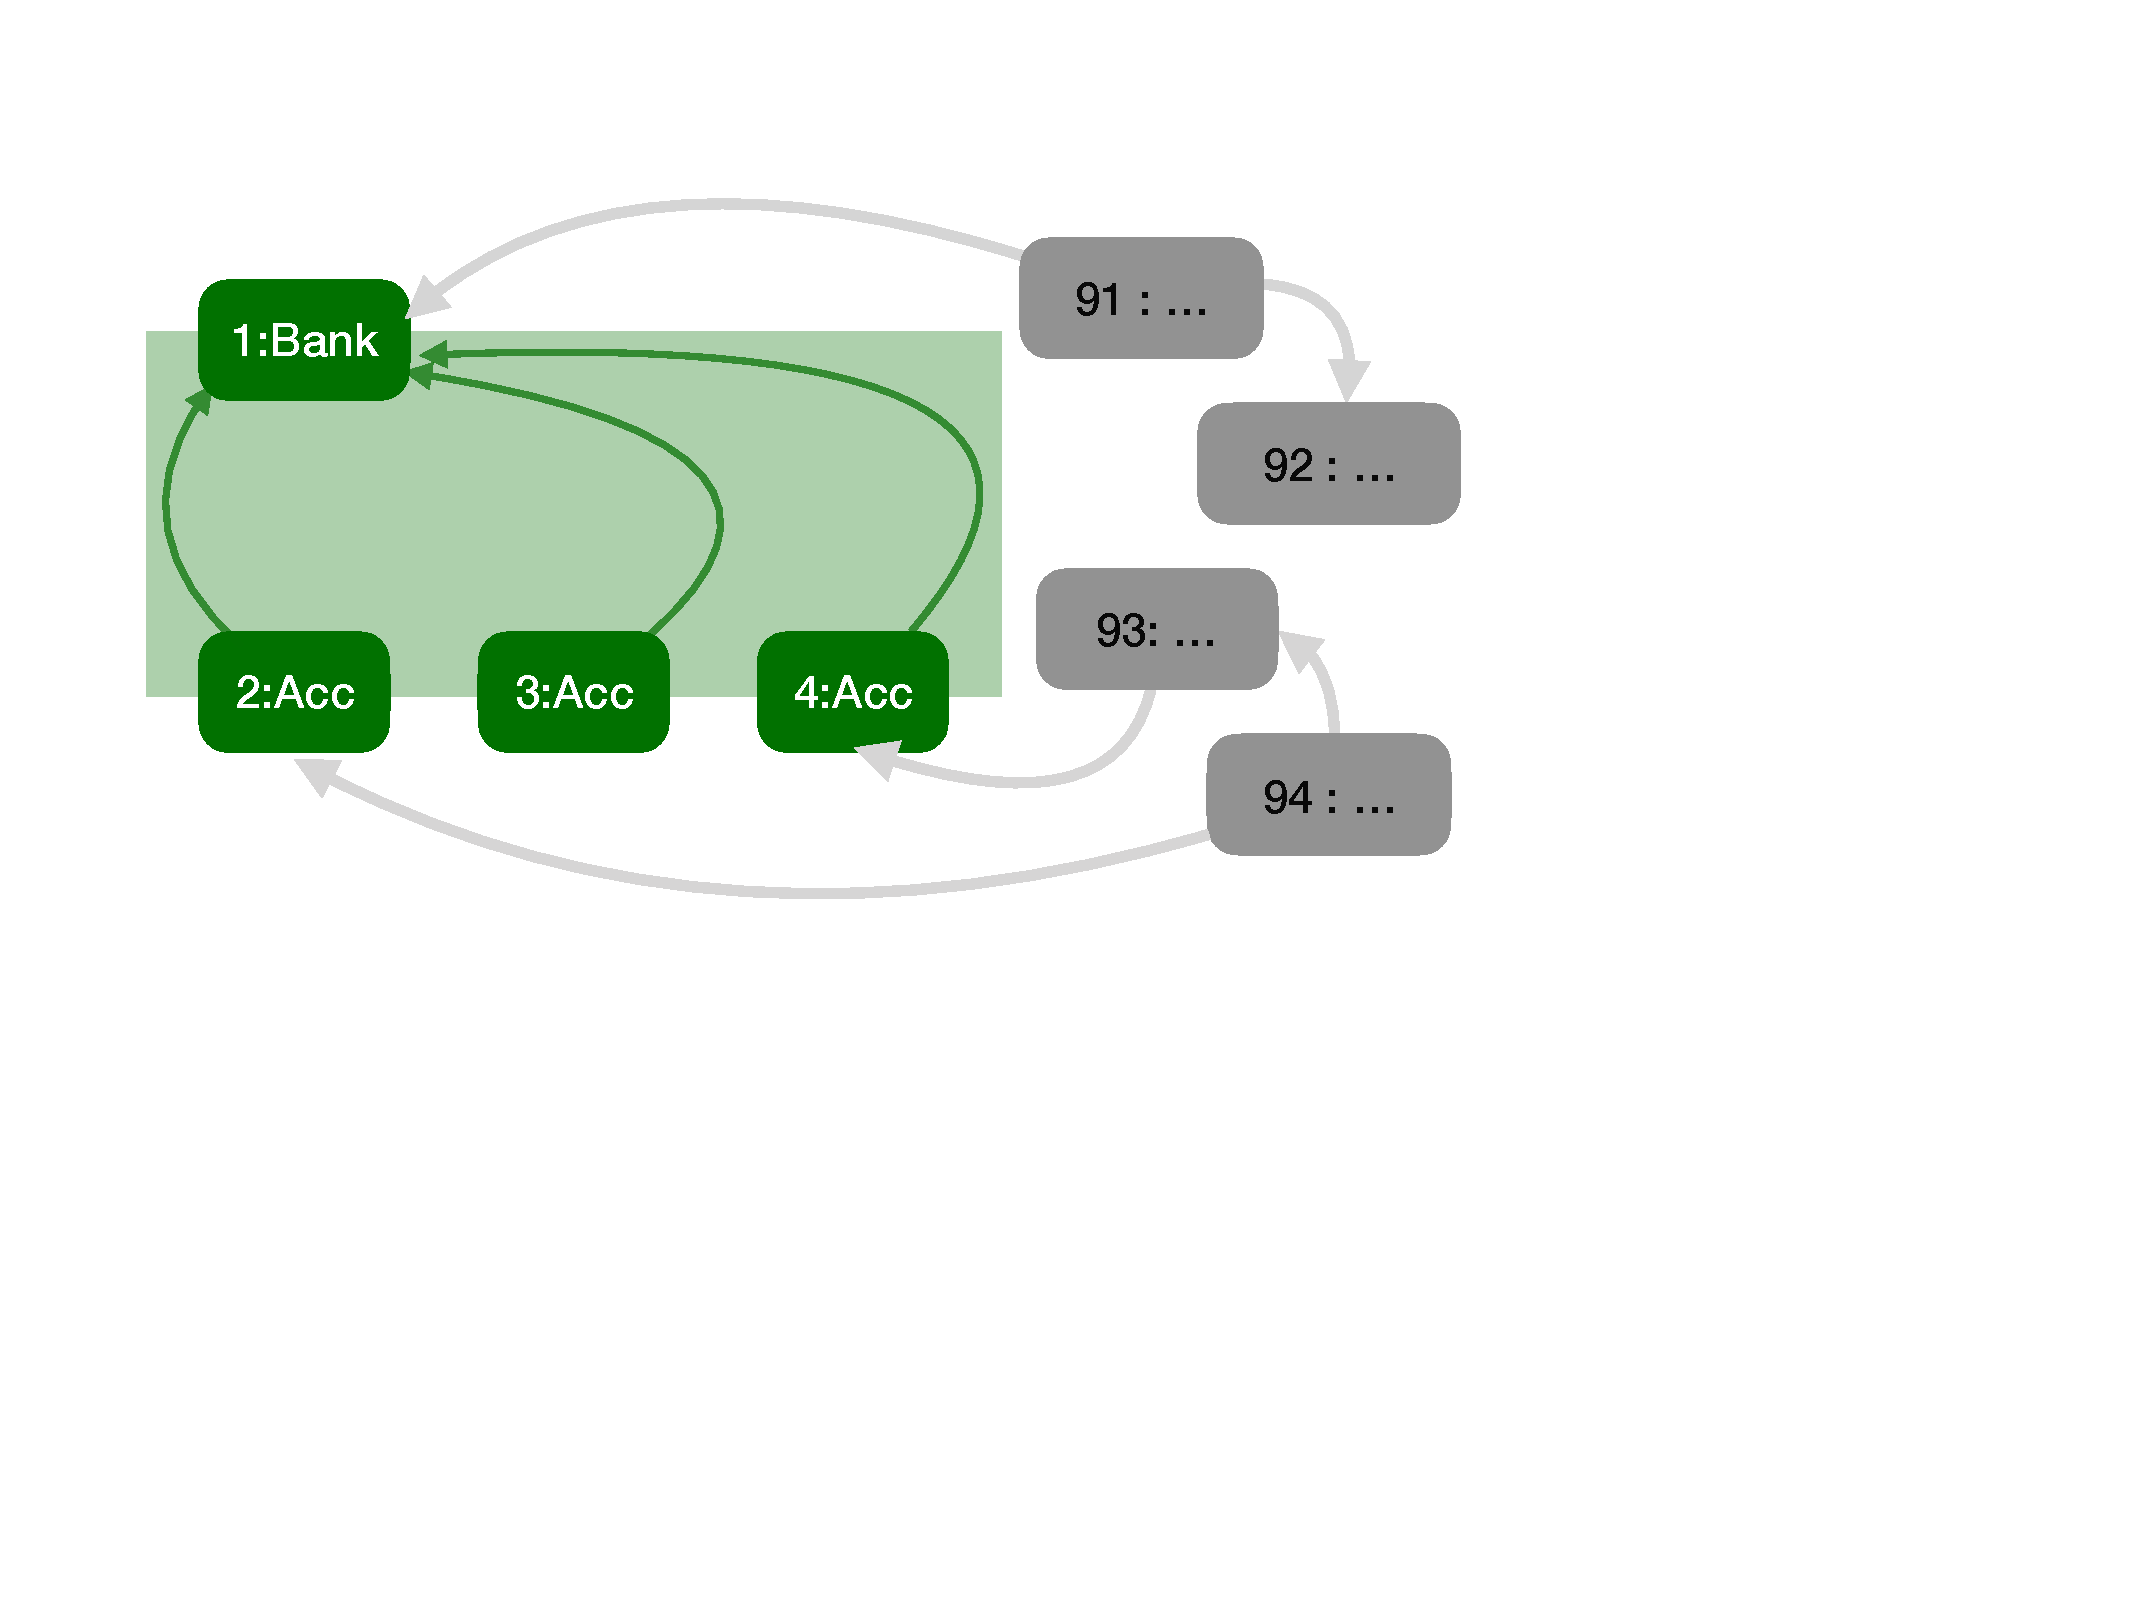
\includegraphics[width=\linewidth, trim=55  330 320 60,clip]{diagrams/BankAccount_version_1.pdf}
   \end{minipage}
 &  
 \begin{minipage}{0.45\textwidth}
 $\sigma_2$\\
  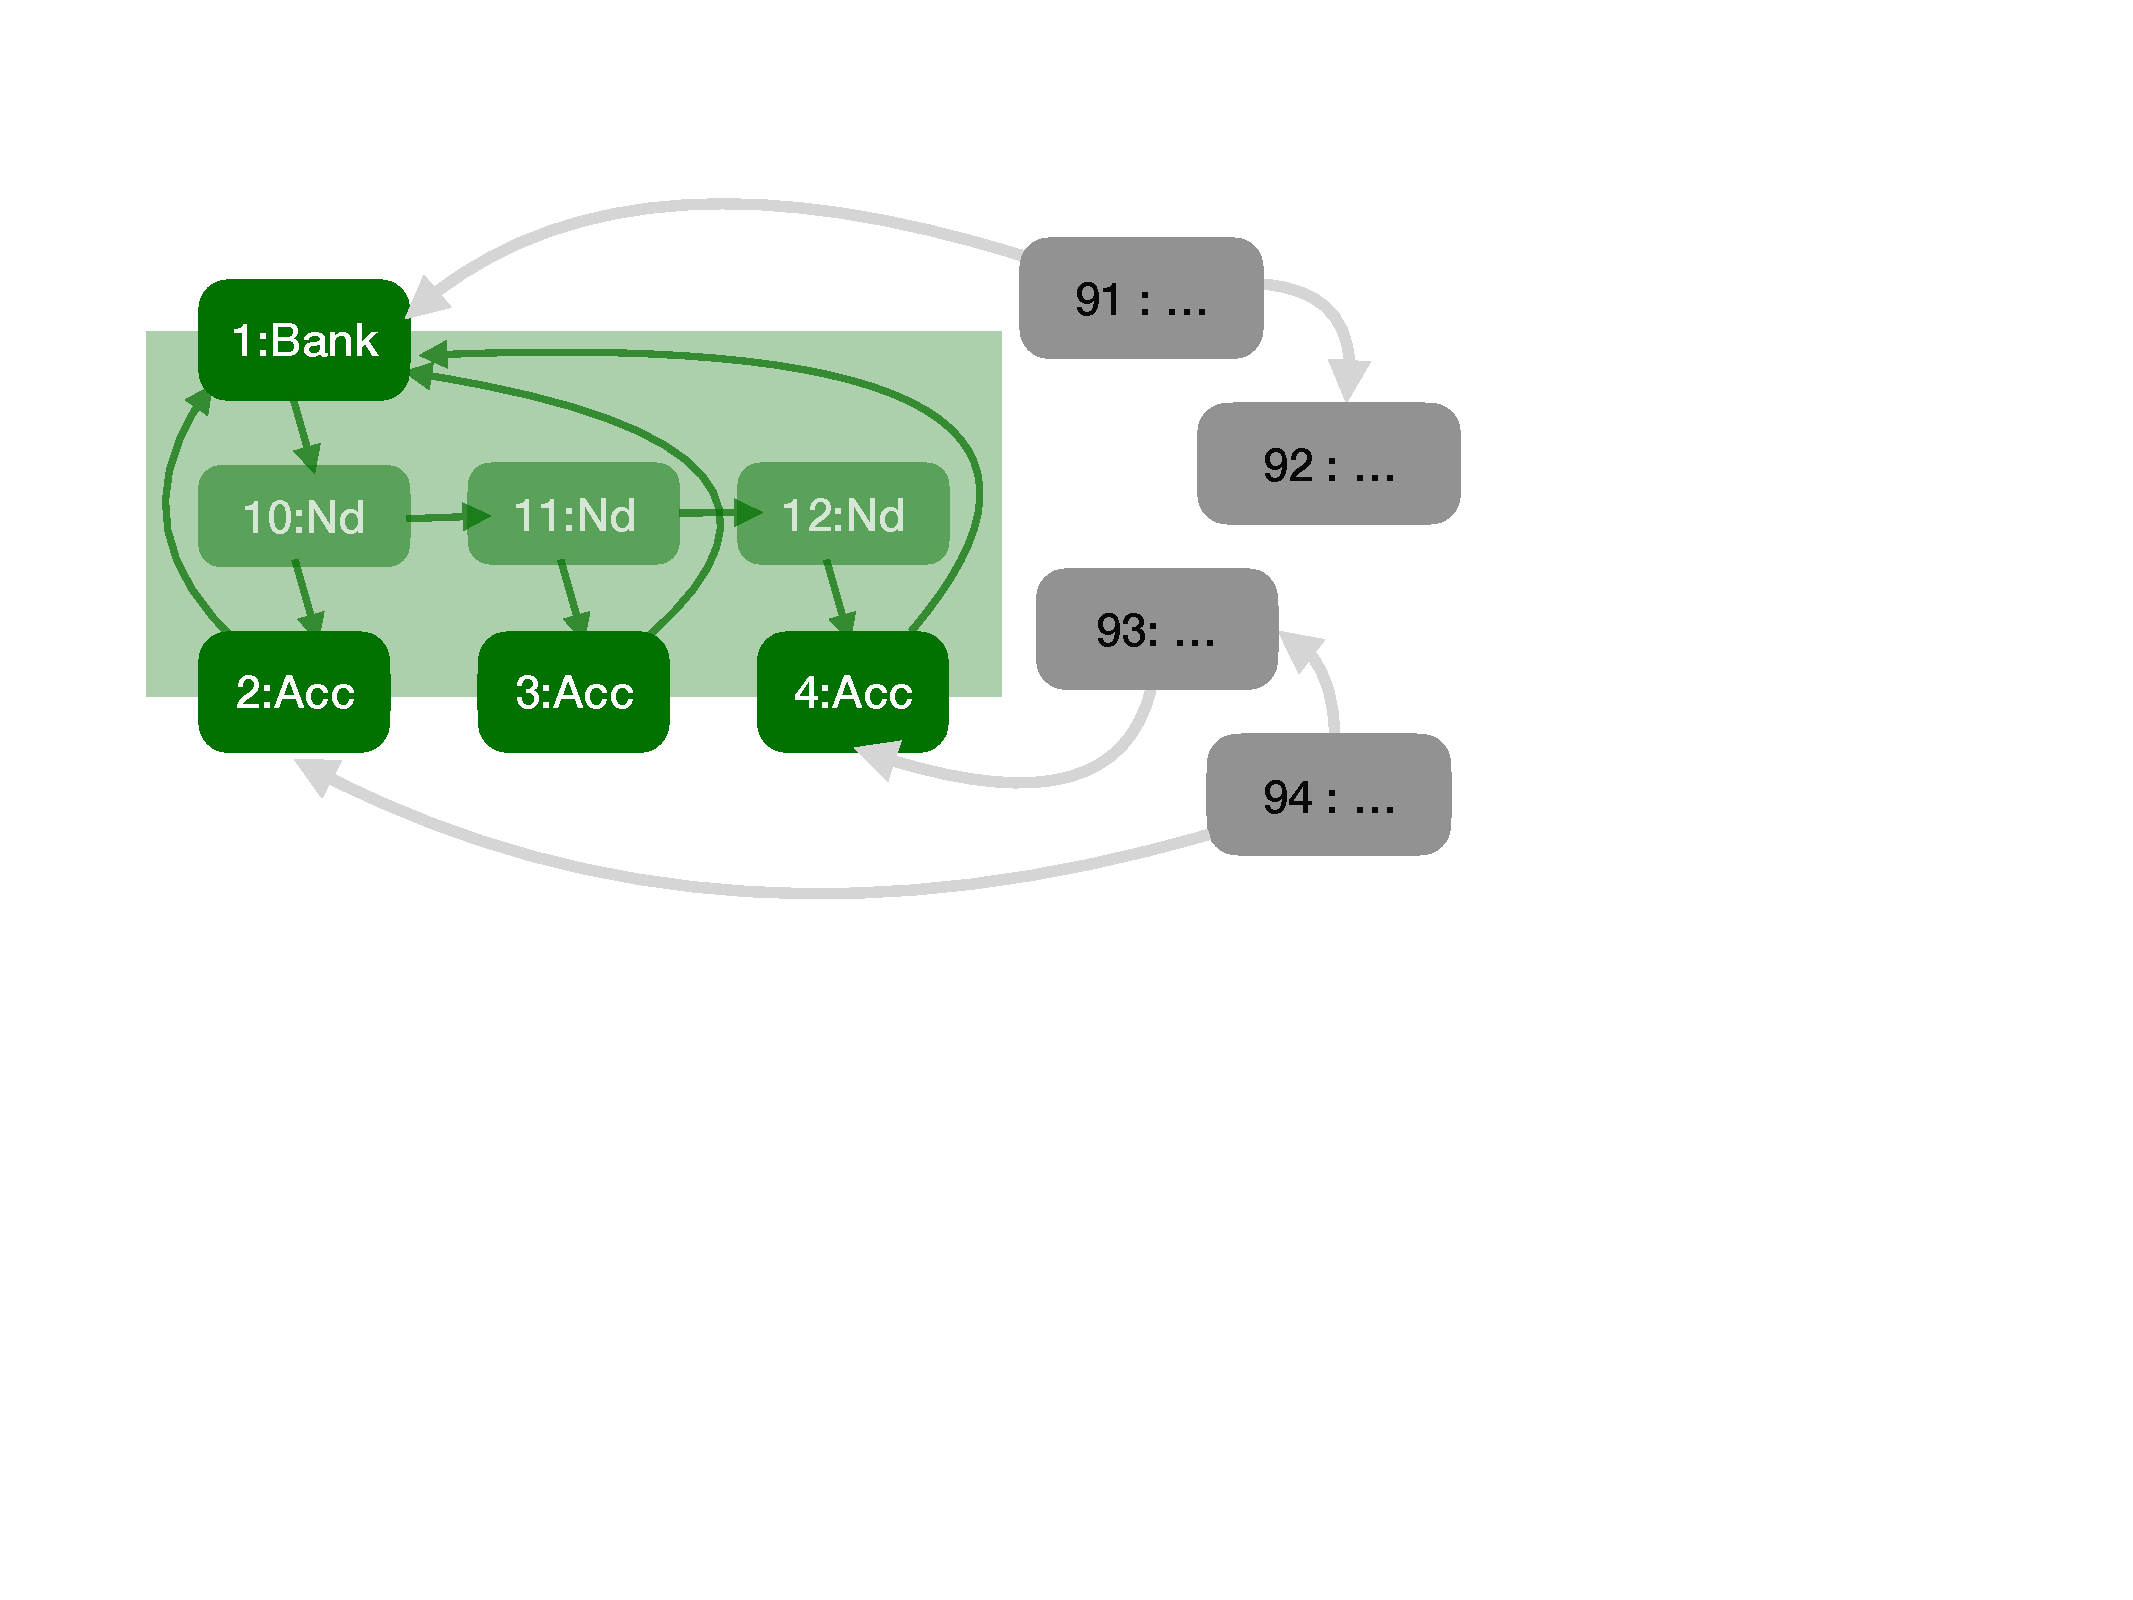
\includegraphics[width=\linewidth, trim=55  330 320 60,clip]{diagrams/BankAccount_version_2.pdf}
   \end{minipage}
\end{tabular}
\caption{Two runtime configurations for the \prg{Bank}/\prg{Account} example. 
}
\label{fig:BakAccountDiagrams}
\end{figure}

\noindent 
For the rest,  assume variable identifiers $\prg{b}_1$, and $\prg{a}_2$--$\prg{a}_4$, and  $\prg{u}_{91}$--$\prg{u}_{94}$ denoting objects \prg{1}, \ \prg{2}--\prg{4},
and   \prg{91}--\prg{94} respectively for both $\sigma_1$ and $\sigma_2$.
That is, for $i$=$1$ or $i$=$2$, $\sigma_i(\prg{b}_1)$=\prg{1}, 
$\sigma_i(\prg{a}_2)$=\prg{2}, $\sigma_i(\prg{a}_3)$=\prg{3},  $\sigma_i(\prg{a}_4)$=\prg{4},  
  $\sigma_i(\prg{u}_{91})$=\prg{91}, $\sigma_i(\prg{u}_{92})$=\prg{92},   
  $\sigma_i(\prg{u}_{93})$=\prg{93}, and $\sigma_i(\prg{u}_{94})$=\prg{94}.



\sdparagraph{Classical Assertions} talk about the contents of the 
local variables (\ie the topmost stack frame), and the 
fields of the various objects (\ie the heap).  
  For example, the assertion  $\ \prg{a}_2.\prg{myBank}$=$\prg{a}_3.\prg{myBank} $, says that
  $\prg{a}_2$ and  $\prg{a}_3$  have the same bank. In fact, this assertion is
  satisfied in both $\sigma_1$ and $\sigma_2$, written formally as\\
  $\strut$ \hspace{1.1cm}  $...,\sigma_1 \ \models \ \prg{a}_2.\prg{myBank}=\prg{a}_3.\prg{myBank}$
  % , $\ \ \ $  and also
%  $\strut$ \hspace{1.1cm}
 \hspace{1cm}   $...,\sigma_2 \ \models \ \prg{a}_2.\prg{myBank}=\prg{a}_3.\prg{myBank}$.
   
 
  The term \prg{x}:\prg{ClassId} says that \prg{x} is an object of class \prg{ClassId}. For example\\
  $\strut$ \hspace{1.1cm}  $...,\sigma_1 \ \models \ \prg{a}_2.\prg{myBank} : \prg{Bank}$.
  
  We support ghost fields~\cite{ghost,Leavens-etal07}, 
   \eg $\prg{a}_1$.\prg{balance} is a physical field in $\sigma_1$ and a ghost field in $\sigma_2$ since in \prg{MBA2} an \prg{Account} does not store its \prg{balance} (as can be seen in appendix~\ref{Bank:appendix}
Fig.~\ref{fig:BanAccImplV2a}). %\sd{The abstract function %this is a term from the ESOP'06 paper from aboove
 % for \prg{balance}  is defined in  the body of class \prg{Account}}  in \prg{MBA2}  \sd{in the obvious way}.


We also support the usual logical connectives, and so, we can express assertions such as \\
$\strut$ \hspace{1.1cm}    $\forall \prg{a}. [ \ \ \prg{a}:\prg{Account} \ \longrightarrow \ \ \prg{a}.\prg{myBank}:\prg{Bank}\ \wedge\  \prg{a}.\prg{balance}\geq 0\ \ ] $ .



\sdparagraph{Permission: Access}
%
Our first holistic assertion, $\CanAccess{\x}{\y}$, asserts that  
object $\x$ has a direct reference to another object $\y$: either one
of $\x$'s fields contains a 
reference to $\y$, or the receiver of the currently executing method is \prg{x}, and \prg{y}
is one of the arguments or a local variable. 
For example:\\
 $\strut$ \hspace{1.1cm}  $...,\sigma_1 \ \models \  \CanAccess{\prg{a}_2}{\prg{b}_1}$
\\
Assuming that  $\sigma_1$ 
is executing the method body corresponding to the call ${\prg{a}_2}$.\prg{deposit}\prg{(}${\prg{a}_3}$,\prg{360}\prg{)},  we 
  have\\
 $\strut$ \hspace{1.1cm}  $...,\sigma_1 \ \models \  \CanAccess{\prg{a}_2}{\prg{a}_3}$, \\
 Namely, during execution of \prg{deposit}, the object  at   $\prg{a}_2$ has access to the object at $\prg{a}_3$, and could,
  if the method body chose to,  call a method on $\prg{a}_3$ , or  store a reference to $\prg{a}_3$ in its own fields.
  %  \sophia{ALL: does this clarify why   we define access to take method execution into account?}
 Note that access is not symmetric, nor transitive:\\
  $\strut$ \hspace{1.1cm}  $...,\sigma_1 \ \not\models \  \CanAccess{\prg{a}_3}{\prg{a}_2}$, \hspace{0.6cm}\\
  $\strut$ \hspace{1.1cm} 
  $...,\sigma_2 \ \models \  \CanAccessTr{\prg{a}_2}{\prg{a}_3}$, \hspace{0.6cm}
 %   $\strut$ \hspace{1.1cm}  
 $...,\sigma_2 \ \not\models \  \CanAccess{\prg{a}_2}{\prg{a}_3}$.


%\james{do we really not also need reachable (transitive closure of access)}
%\susan{we don't seem to need transitivity in any of the examples}
%\sophia{We do not want transitivity, our policies where access is in the conclusion would become too weak.}

\sdparagraph{Control: Calls}
%
The  assertion $\Calls {\x} {\y} {\m} {\zs}$
% \sophia{it said " is more-or-less the control flow analogue of
% the access assertion" -- that is a nice simile, but is it true?\kjx{I
% think it's true}} 
 holds 
in program states where a method on object 
${\x}$ makes a method call ${\y}.{\m}({\zs})$ --- that is it calls method 
{\m} with object {\y} as the receiver, and with arguments {\zs}.
For example, \\
 $\strut$ \hspace{1.1cm}  $...,\sigma_3 \models \  \Calls {\x}{\prg{deposit}}  {\prg{a}_2} { {\prg{a}_3},\prg{360}}$.\\
 %{{...}} {\prg{a}_2}} {\prg{deposit}} {\prg{(}{\prg{a}_3},\prg{100.00}\prg{)}}$.\\
 means that the receiver in %configuration
 $\sigma_3$ is \x, and the next statement to be executed 
 is  $\prg{a}_2.\prg{deposit}{\prg{(}}\prg{a}_3,\prg{360}{\prg{)}}$.
 

%% \sdparagraph{Authority --  Changes and Internal/External}\sophia{Is it good to put these together?}
%% The assertion $\Changes{\prg{e}}$  holds when the value of {\prg{e}}
%% in the next configuration is different to the value in the current configuration.
%% For example, if the code being executed in $\sigma_1$ started with $\acc_2.\bal=\acc_2.\bal+\prg{100.00}$, then:\\
%%   $\strut$ \hspace{1.1cm}  $..., \sigma_1 \ \models \  \Changes {\acc_2.\bal}$.\\
%%   Moreover, the assertion $\External {\prg{e}}$ expresses that the object {\prg{e}} does not belong to the module under consideration. 
%%   For example, \\
%% $\strut$ \hspace{1.1cm}  $\M_{AB2}\mkpair ..., \sigma_2 \ \models \ \External{\pu_{92}}$,
%% %$\strut$ 
%% \hspace{1cm}  $\M_{AB2}\mkpair ..., \sigma_2 \ \not\models \ \External{\acc_2}$, \\
%% $\strut$
%%  \hspace{1.1cm}  $\M_{AB2}\mkpair ..., \sigma_2 \ \not\models \ \External{\pb_{1}.\prg{ledger}}$\\
%% Notice the use of the \emph{internal} module, $\M_{AB2}$, needed to judge which objects are internal, and which are external.
 

\sdparagraph{Space: {In}}
The space assertion $\Using{\A}{\SF}$ establishes validity of $\A$ 
 in a configuration  restricted to the 
objects from the set \SF.
% In other words, it restricts the set of objects which may be used to establish property \A. 
For example, 
if  object \prg{94}  is included in $\SF_1$ but not in  $\SF_2$, then we   have\\ 
 $\strut$ \hspace{1.1cm}  $..., \sigma_1 \ \models \ \Using{ (\exists \prg{o}.\,\CanAccess{\prg{o}}{\acc_4})}{\SF_1}$
$\strut$ \hspace{0.2cm}  
 $\strut$ \hspace{1.1cm}  $..., \sigma_1 \ \not\models \ \Using{ (\exists \prg{o}.\,\CanAccess{\prg{o}}{\acc_4})} {\SF_2}$.\\
 The set \SF\ in the assertion $\Using{\A}{\SF}$  is therefore {\em not} the footprint of   $\A$;
  it is more like the \emph{fuel}\cite{stepindex}  given to establish that assertion. Note that  $..., \sigma \ \models \Using {\A} {\SF}$ does not imply  
  $..., \sigma \ \models \A$  nor does it imply   $..., \sigma \ \models \Using {\A} {\SF\cup\SF'}$.
  The other direction of the implication does not hold either.
% \james{would still like  a one sentence motivating/justifying ``with''. Why do we need it}

\sdparagraph{Time: Next, Will, Prev, Was}
We support several operators from temporal
logic: ($\Next \A$, $\Future \A$,  $\Prev \A$, and $\Past \A$) to
talk about the future or the past in one or more number steps.
The assertion $\Future \A$ expresses that %after one or more execution steps
$\A$ will hold in one or more steps. For example, 
taking $\sigma_4$ to be similar to  $\sigma_2$, the next statement to be executed 
to be  $\prg{a}_2.\prg{deposit}{\prg{(}}\prg{a}_3,\prg{360}{\prg{)}}$, and 
$\M_{BA2}\mkpair ..., \sigma_4 \ \models \  \acc_2.\bal=\prg{60}$, then\\ 
 $\strut$ \hspace{1.1cm}  $\M_{BA2}\mkpair ..., \sigma_4 \ \models \ \Future{ {\acc_2.\bal}=\prg{420}}$.\\
Notice the use of the \emph{internal} module, $\M_{AB2}$, needed for looking up the method body of \prg{deposit}.
  
\sdparagraph{Viewpoint: --  External}
%% The assertion $\Changes{\prg{e}}$  holds when the value of {\prg{e}}
%% in the next configuration is different to the value in the current configuration.
%% For example, if the code being executed in $\sigma_1$ started with $\acc_2.\bal=\acc_2.\bal+\prg{100.00}$, then:\\
%%   $\strut$ \hspace{1.1cm}  $..., \sigma_1 \ \models \  \Changes {\acc_2.\bal}$.\\
The assertion $\External {\prg{x}}$ expresses that the object at {\prg{x}} does not belong to the module under consideration. 
  For example, \\
$\strut$ \hspace{1.1cm}  $\M_{AB2}\mkpair ..., \sigma_2 \ \models \ \External{\pu_{92}}$,
%$\strut$ 
\hspace{1cm}  $\M_{AB2}\mkpair ..., \sigma_2 \ \not\models \ \External{\acc_2}$, \\
$\strut$
 \hspace{1.1cm}  $\M_{AB2}\mkpair ..., \sigma_2 \ \not\models \ \External{\pb_{1}.\prg{ledger}}$\\
The \emph{internal} module, $\M_{BA2}$, is needed to judge which objects are internal or external.
 
\sdparagraph{Change and Authority:} We have used 
$\Changes {}$ 
in our \Chainmail assertions in section~\ref{sect:motivate:Bank}, as in
 $\Changes  {\acc.\prg{balance}}$. Assertions that talk about change, or give conditions for change
to happen are fundamental for security; the ability to cause change is called \emph{authority} in \cite{MillerPhD}. 
We could encode change using the other features of \Chainmail, namely, for any expression \e:\\
$\strut$ \hspace{1.1cm}
$\Changes {\e}$\  \ $\equiv$\ \ $\exists v. [\ \e=v \wedge \Next {\neg ( \prg{e}=v)}\ ]$.\\
and similarly for assertions.


%\sophia{The observer pattern example is very nice, but unfortunately we cannot use it, because the
%calls are internal, and therefore not visible in the current system.}
%For example, a part of the observer pattern is that when
%a subject is notified of a change, then the observer must
%be told to update itself.    We can write this from the
%subject's perspective, looking forwards:
%
%\begin{lstlisting}
%  Call(_,subject,notify,_) --> Will(Call(subject,observer,update,_))
%\end{lstlisting}
%
%\noindent meaning that once notify is called on a subejct, then its
%observer will be updated sometime in the future.  We can write a very
%similar specification for an observer, looking backwards.
%
%\begin{lstlisting}
%  Call(subject,observer,update,_) --> Was(Call(_,subject,notify,_))
%\end{lstlisting}
%
%\noindent meaning that if a subject updates an observer, that subject
%have been notified sometime previously. We could tighten each
%specifaction, so that the update must immediately follow the
%notification, by replacing $\Future \A$ or $\Past \A$ with 
%$\Next \A$ or $\Prev \A$.

\sdparagraph{Putting these together} We now look at some composite assertions which use  
 several features from above. The assertion below 
says that if the statement to be executed is   $\acc_2.\prg{deposit}\prg{(}\acc_3,\prg{60}\prg{)}$,
then the balance of $\acc_2$ will eventually change:\\
 $\strut$ \hspace{1.1cm}  
 $\M_{BA2}\mkpair ..., \sigma_2 \ \models \ {\Calls {..}   {\prg{deposit}} {\acc_1} {\acc_2,\prg{60}} } \longrightarrow {\Future{ \Changes {\acc_2.\bal}}}$.

\vspace{.2cm}
 
We now look deeper into the meaning of space assertions, $\Using{\A}{\SF}$. They allow us to characterise the set of objects which have authority over certain effects (here $\A$). In particular,  the assertion   $\Using {\Future {\A}} {\SF}$  does two things: it requires that $\A$ will hold in the future, and that the objects which cause the effect which will make $\A$ valid, are   included in \SF.
Knowing who has, and who has not, authority over properties or data is a fundamental concern of robustness
\cite{MillerPhD}. Notice that the authority is a set, rather than a single object: quite often it takes \emph{several objects in concert}
 to achieve an effect.


Now, consider assertions (2) and (3) from the previous section. They both have the form\\
 $\strut$ \hspace{1.1cm}  $\Future {\Using {\A} {\SF}}\ \longrightarrow P(\SF)$,\\
  where $P$ is some property over a set. These assertion say, that if ever in the future $\A$ becomes valid, and if the objects involved in making $\A$ valid are included in $\SF$, then $\SF$ must satisfy $P$. Such assertions can be used to restrict whether $\A$ will become valid. Namely, if we have some execution which only involves objects which do not satisfy $P$, then we know that the execution will not ever make $\A$ valid.

%\susan{I don't know where m and m2 come from. We haven't seen them up to now and I don't  see why they are needed in this story.}
 In general, $\Future {\Using {\A} {\SF}}$ is different from
  $\Using {\Future {\A}} {\SF}$.  Namely, in the former assertion, $\SF$ must contain
   the objects involved in reaching the future configuration as well as the objects needed to
    then establish validity of $\A$ in that future configuration. In the latter assertion, 
     $\SF$ need only contain the objects needed to establish $\A$ in that future configuration.
  For example, take $\SF_1$ to consist of objects \prg{1}, \prg{2}, \prg{4}, \prg{93}, and \prg{94},
  and $\SF_2$ to consist of objects \prg{1}, \prg{2}, \prg{4}. 
  %Assume   that $\sigma_1$ contains the
  % call $\prg{m()}$ with receiver $\pu_{94}$ and that the code of \prg{m} and \prg{m2} is as above. 
  Then\\
  $\strut$ \hspace{1.1cm}  $\M_{BA1}\mkpair ..., \sigma_1 \ \models \ \Using {\Future{ \Changes {\acc_2.\bal}}} {\SF_1}$\\
   $\strut$ \hspace{1.1cm}  $\M_{BA1}\mkpair ..., \sigma_1 \ \not\models \ \Using {\Future{ \Changes {\acc_2.\bal}}} {\SF_2}$\\
 $\strut$ \hspace{1.1cm}  $\M_{BA1}\mkpair ..., \sigma_1 \ \models \ \Future{ \Using {\Changes {\acc_2.\bal}} {\SF_2}}$\

%%\vspace{.2in} 
%\sophia{While
%many  individual
%features of \Chainmail can  be found also in other work, we
%%claim that their  combination as well as
%%their application in the specification of open systems are novel.
%argue that their power and novelty for specifying open systems lies in their careful
%  combination}
 
\sdparagraph{In summary,} in addition to classical 
logical connectors and classical assertions over the contents of the heap and the stack, 
our holistic assertions draw from some concepts from object capabilities
($\CanAccess{\_}{\_}$  for  permission; {$\Calls {\_} {\_} {\_} {\_}$ and  $\Changes{\_}$ for
authority) 
as well as temporal logic ($\Future \A$, $\Past \A$ and friends), and the relation of
our spatial connective ($\Using{\A}{S}$)  with ownership and effect
systems \cite{typeEffect,ownalias,ownEncaps}.

The next two sections  discuss the semantics of \Chainmail. Section \ref{sect:formal}
contains an overview of the formal model and section \ref{sect:assertions} focuses on the most important part of \Chainmail : assertions.

%its most important aspect being assertions, whose semantics are in section  \ref{sect:assertions}.

%\james{somewhere, should we say something like: the goal is
%  to allow wholistic specifations with as extra little machinery as
%  possible over a basic Hoare language}.





\section{Overview of the Formal foundations}
\label{sect:formal}
We now give an overview of the formal model for \Chainmail. In section \ref{sect:overviewmodel} we 
introduce  the shape of the judgments used to give semantics to \Chainmail, while in section \ref{sect:PL} 
we describe the most salient aspects of an underlying programming language used in \Chainmail.

\subsection{\Chainmail\ judgments}
\label{sect:overviewmodel}
%\section{Overview of the \Chainmail\  formal model}
% \subsection{The Open World}

Having outlined the ingredients of our holistic specification
language, the next question to ask is: When does a module $\M$ satisfy
a holistic assertion $\A$?  More formally: when does
$\M \models \A$ 
hold? 
  
Our answer has to reflect the fact that we are dealing with an rece
\emph{open  world},  where  $\M$, our module, may be
linked with \textit{arbitrary untrusted code}.
%
%
%% \sd{Note that we use the term \emph{module} to talk about repositories of code; in this work modules are mappings from
%% class identifiers to class definitions.}
%
%
To % skipped the discussion of what a module is
 model the open world, we consider
 pairs of modules, 
$\M \mkpair {\M'}$,  where $\M$ is the module 
whose code is supposed to satisfy the assertion,
and $\M'$  is  another % wused to say \textit{any}  -- but why?
 module which exercises
the functionality of $\M$. We call our module $\M$ the {\em internal} module, and
 $\M'$ the {\em external} module, which represents potential
 attackers or adversaries.
     
We can now answer the question: $\M \models \A$ 
 holds if for all further, {\em potentially adversarial}, modules $\M'$ and in  all runtime configurations $\sigma$ which may be observed as arising from the  execution of the code of $\M$ combined with that of $\M'$, the assertion $\A$ is satisfied. More formally, we define:\\
$~ \strut  \hspace{1.3in} \M \models \A \ \ \  \ \ \ \ \ \mbox{
if               } \ \ \  \ \ \  \  \forall \M'.\forall \sigma\in\Arising
{\M \mkpair  {\M'}}. [\ \M \mkpair  {\M'},\sigma \models \A\ ]$.  \\
Module $\M'$ represents all possible clients of {\M}.  As it is arbitrarily chosen, it reflects the open world nature of our specifications.% 

%% \sophia{Is is sentence superfluous now?.}
%% \sophia{In contrast to what we said on Friday's conf call we do not need to put any restrictions
%% on $\M'$ -- not even disjointness is required.}
%% \kjx{OK so in the \textbf{next iteration} we can just replace M;M' with a ' operator applied to any module\ldots}

The judgement $\M \mkpair  {\M'},\sigma \models \A$ means that  
assertion $\A$ is satisfied by  $\M \mkpair  {\M'}$ and $\sigma$.  
As in traditional specification languages \cite{Leavens-etal07,Meyer92}, satisfaction is judged 
in the context of a runtime configuration $\sigma$; but in addition, it is judged in the context of the internal and external modules.
%Satisfaction is also  judged in the context of modules; t
These are used to find   abstract functions defining ghost fields as well as  method bodies
needed when judging validity of temporal assertions such as
$\Future {\_}$.} %: the modules contain the code necessary to reach those configurations.

We distinguish between internal and external modules. This offers two advantages:
First, 
\Chainmail\ includes the ``$\External{\prg{o}}$'' assertion to require
that an object belongs to the external module, as in the Bank
Account's assertion (2) and (3) in
section~\ref{sect:motivate:Bank}. Second, we adopt a version of
visible states semantics \cite{MuellerPoetzsch-HeffterLeavens06,larch93,Meyer97}, treating all
executions within a module as atomic.
We only record runtime configurations which are {\em external}
 to module $\M$, \ie those where the
 executing object (\ie the current receiver) comes from module $\M'$.
 Execution % is  a judgment of 
 has the form\\
 $~ \strut  \hspace{1.3in}    \M \mkpair  {\M'},\sigma \leadsto \sigma'$\\  
% $\M \mkpair  {\M'},\sigma \leadsto \sigma'$\\  
where we ignore all intermediate steps
 with receivers  internal to $\M$. 
 % removed the below as it appears in next section.
%Similarly, when considering $\Arising {\M \mkpair  {\M'}}$, \ie the configurations arising from 
%executions in $\M \mkpair  {\M'}$, we can take method bodies defined in $\M$ or in $\M'$, but we will only consider the runtime 
%configurations which are external to $\M$.
%
In the next section we  shall 
outline the underlying programming language, and
define the judgment  $\M \mkpair  {\M'},\sigma \leadsto \sigma'$ and the set 
$\Arising {\M \mkpair  {\M'}}$.
 





\subsection{An underlying programming language, \LangOO}
\label{sect:PL}
\renewcommand{\appref}[1]{, c.f. Appendix, Def.\,\ref{#1}}
 
%As was have seen, \Chainmail assertions not only talk about the contents of the current state (stack frame and heap),
%but they also talk about future and past states, Therefore, 
The meaning of \Chainmail assertions is parametric with an
underlying object-oriented programming language, with modules  as repositories of code, classes with fields, methods and
ghostfields, objects described by classes, a way to link  modules into larger ones, and a concept of 
program execution\footnote{We believe that \Chainmail can be applied to 
any language with these features.}.

We have developed   \LangOO, a \jm{deterministic and} minimal such object-oriented language, which we
outline in  this section. 
We  describe the novel aspects of \LangOO, and 
summarise the more conventional parts, relegating  full, and mostly unsurprising,
definitions %for  \LangOO~appear 
to Appendix \ref{app:LangOO}.
 

Modules are central to \LangOO, as they are to \Chainmail. As modules are repositories
of code, we adopt the common formalisation of modules as maps from 
class identifiers to class definitions\appref{defONE}. We use the terms module and component in an
analogous manner to class and object respectively.  \LangOO is untyped 
\sophia{for several reasons. Many popular programming languages are untyped.
The external module might be untyped, and so it is more
general to consider everything as untyped.
Finally, 
a solution that works for an untyped language %(doesnt depend on types) 
will also apply to a typed language, while the converse is not true.
}
%, where we link with external modules which come without any
%guarantees.

 Class definitions consist of field, method and ghost field declarations\appref{def:syntax:classes}.
Method bodies are sequences of 
statements, which  can be field reads or field assignments, object
creation, method calls, and return statements. 
%All else, \eg booleans, conditionals, loops,  can be encoded.
Fields are private in the sense of C++ or Java: they can only be read or
written by methods of the current class.
This is enforced by the operational semantics, \cf Fig.~\ref{fig:Execution}.
We  discuss ghost fields in the next section.

Runtime configurations, $\sigma$,  contain   all the usual information about execution snapshots: the heap, and a
stack of frames. 
% sd dropped fillowing sentence as it appears afterwards
%The code to be executed is kept as part of the runtime configuration:
%
Each frame consists of a continuation, \prg{contn}, describing the remaining code to be executed by the
frame, and a map from
variables to values. Values are either addresses or sets of addresses; sets 
are needed to deal with assertions which quantify over sets of
objects, such as assertions
(1) and (2) from Section \ref{sect:motivate:Bank}.
% 
We define \emph{one-module} execution  through a judgment of the form $\M, \sigma \leadsto \sigma'$ in Appendix~\ref{app:LangOO}, Fig.~\ref{fig:Execution}. 
%
  

%\subsection{\sdf{Modules satisfying assertions}}
%
%Finally, we define satisfaction of assertions by modules: a module
%$\M$ satisfies an assertion $\A$ if for all other potential modules $\M'$, in all configurations arising from executions of $\M\mkpair\M'$, the assertion $\A$ holds.

%\begin{definition}
%\label{def:module_satisfies}
%For any module $\M$, and  assertion $\A$, we define:
%\begin{itemize}
%\item
%$\M \models \A \ \ \  \ \ \ \ \ \mbox{
%if               } \ \ \  \ \ \  \  \forall \M'.\forall \sigma_0 \in \Initial{\M \mkpair \M'}.\forall\sigma\in\Arising{\M \mkpair  {\M'}, \sigma_0}. [\ \M \mkpair  {\M'}, \sigma_0 , \sigma \models \A\ ]$
%\end{itemize}
%\end{definition}
  
  

\subsection{\sdf{Linking and two-state execution}}

We define a module linking operator \  $\link$ \  so that
$\M\link\M'$ is the union of the two modules, provided that their domains are disjoint\appref{def:link}.
 %
As we said in Section \ref{sect:overviewmodel}, we distinguish  between the internal and external module. \sophia{We consider execution  from the view of the
external module, and treat}  execution of 
methods from the internal module as atomic. For this, we define \emph{two-module execution}  based on
one-module execution as follows:

%Susan: I don't understand this when n = 2
\begin{definition}
\label{def:execution:internal:external}
\label{def:module_pair_execution} 
Given runtime configurations $\sigma$,  $\sigma'$,  and a module-pair $\M \mkpair \M'$ we define
execution where $\M$ is the internal, and $\M'$ is the external module as below:
 
\begin{itemize}
\item
$\M \mkpair \M', \sigma \leadsto \sigma'$ \IFF
there exist  $n\geq 2$ and runtime configurations $\sigma_1$,  ...
$\sigma_n$, \\such that
\begin{itemize}
\item
$\sigma$=$\sigma_1$,\ \  \ \ and\ \ \ \ $\sigma_n=\sigma'$.
\item
$\M \link \M', \sigma_i \leadsto \sigma_{i+1}$,\  \  for $1\leq i \leq n\!-\!1$
\item
$\ClassOf{\this} {\sigma}\not\in dom({\M})$,  \ \  \ \ and\ \ \ \
$\ClassOf{\this} {\sigma'} \not\in dom({\M})$,
\item
 $\ClassOf{\this} {\sigma_i} \in dom({\M})$,\ \ \ \ for $2\leq i \leq n\!-\!\Mrrz{1}$
\end{itemize}
\end{itemize}

\end{definition}
 
In the definition above,  $\ClassOf {\x} {\sigma} $ looks up the class of the object \sophia{stored} at \x\appref{def:interp}.
% If  $n$  has the value $2$, %. In this case the final bullet is trivial and  
%then  there exists a direct, external transition from $\sigma$ to $\sigma'$.  
 For example, for $\sigma_4$ as in Section \ref{sect:chainmail} whose next statement to be executed 
 is  $\prg{a}_2.\prg{deposit}{\prg{(}}\prg{a}_3,\prg{360}{\prg{)}}$,  we would have 
 a sequence of configurations $\sigma_{41}$, ... $\sigma_{4n}$,  $\sigma_{5}$ so that the
  one-module execution gives
 $\M_{BA2}, \sigma_4 \leadsto \sigma_{41} \leadsto \sigma_{42} ... \leadsto \sigma_{4n}   \leadsto \sigma_{5}$.
This would correspond to an atomic evaluation in the two-module execution: \  \
 $\M_{BA2}\mkpair \M', \sigma_4 \ \leadsto \sigma_5$ (see Fig.\ref{fig:VisibleStates}; \sophia{where blue stands for $\sigma(this)\!\in\!M_1$,%
   and  orange for $\sigma(this)\!\in\!M_2$}).


\begin{figure}[htb]
  \vspace*{-2.5mm}
  \begin{center}
   \begin{minipage}{0.80\textwidth}
     \begin{center}
       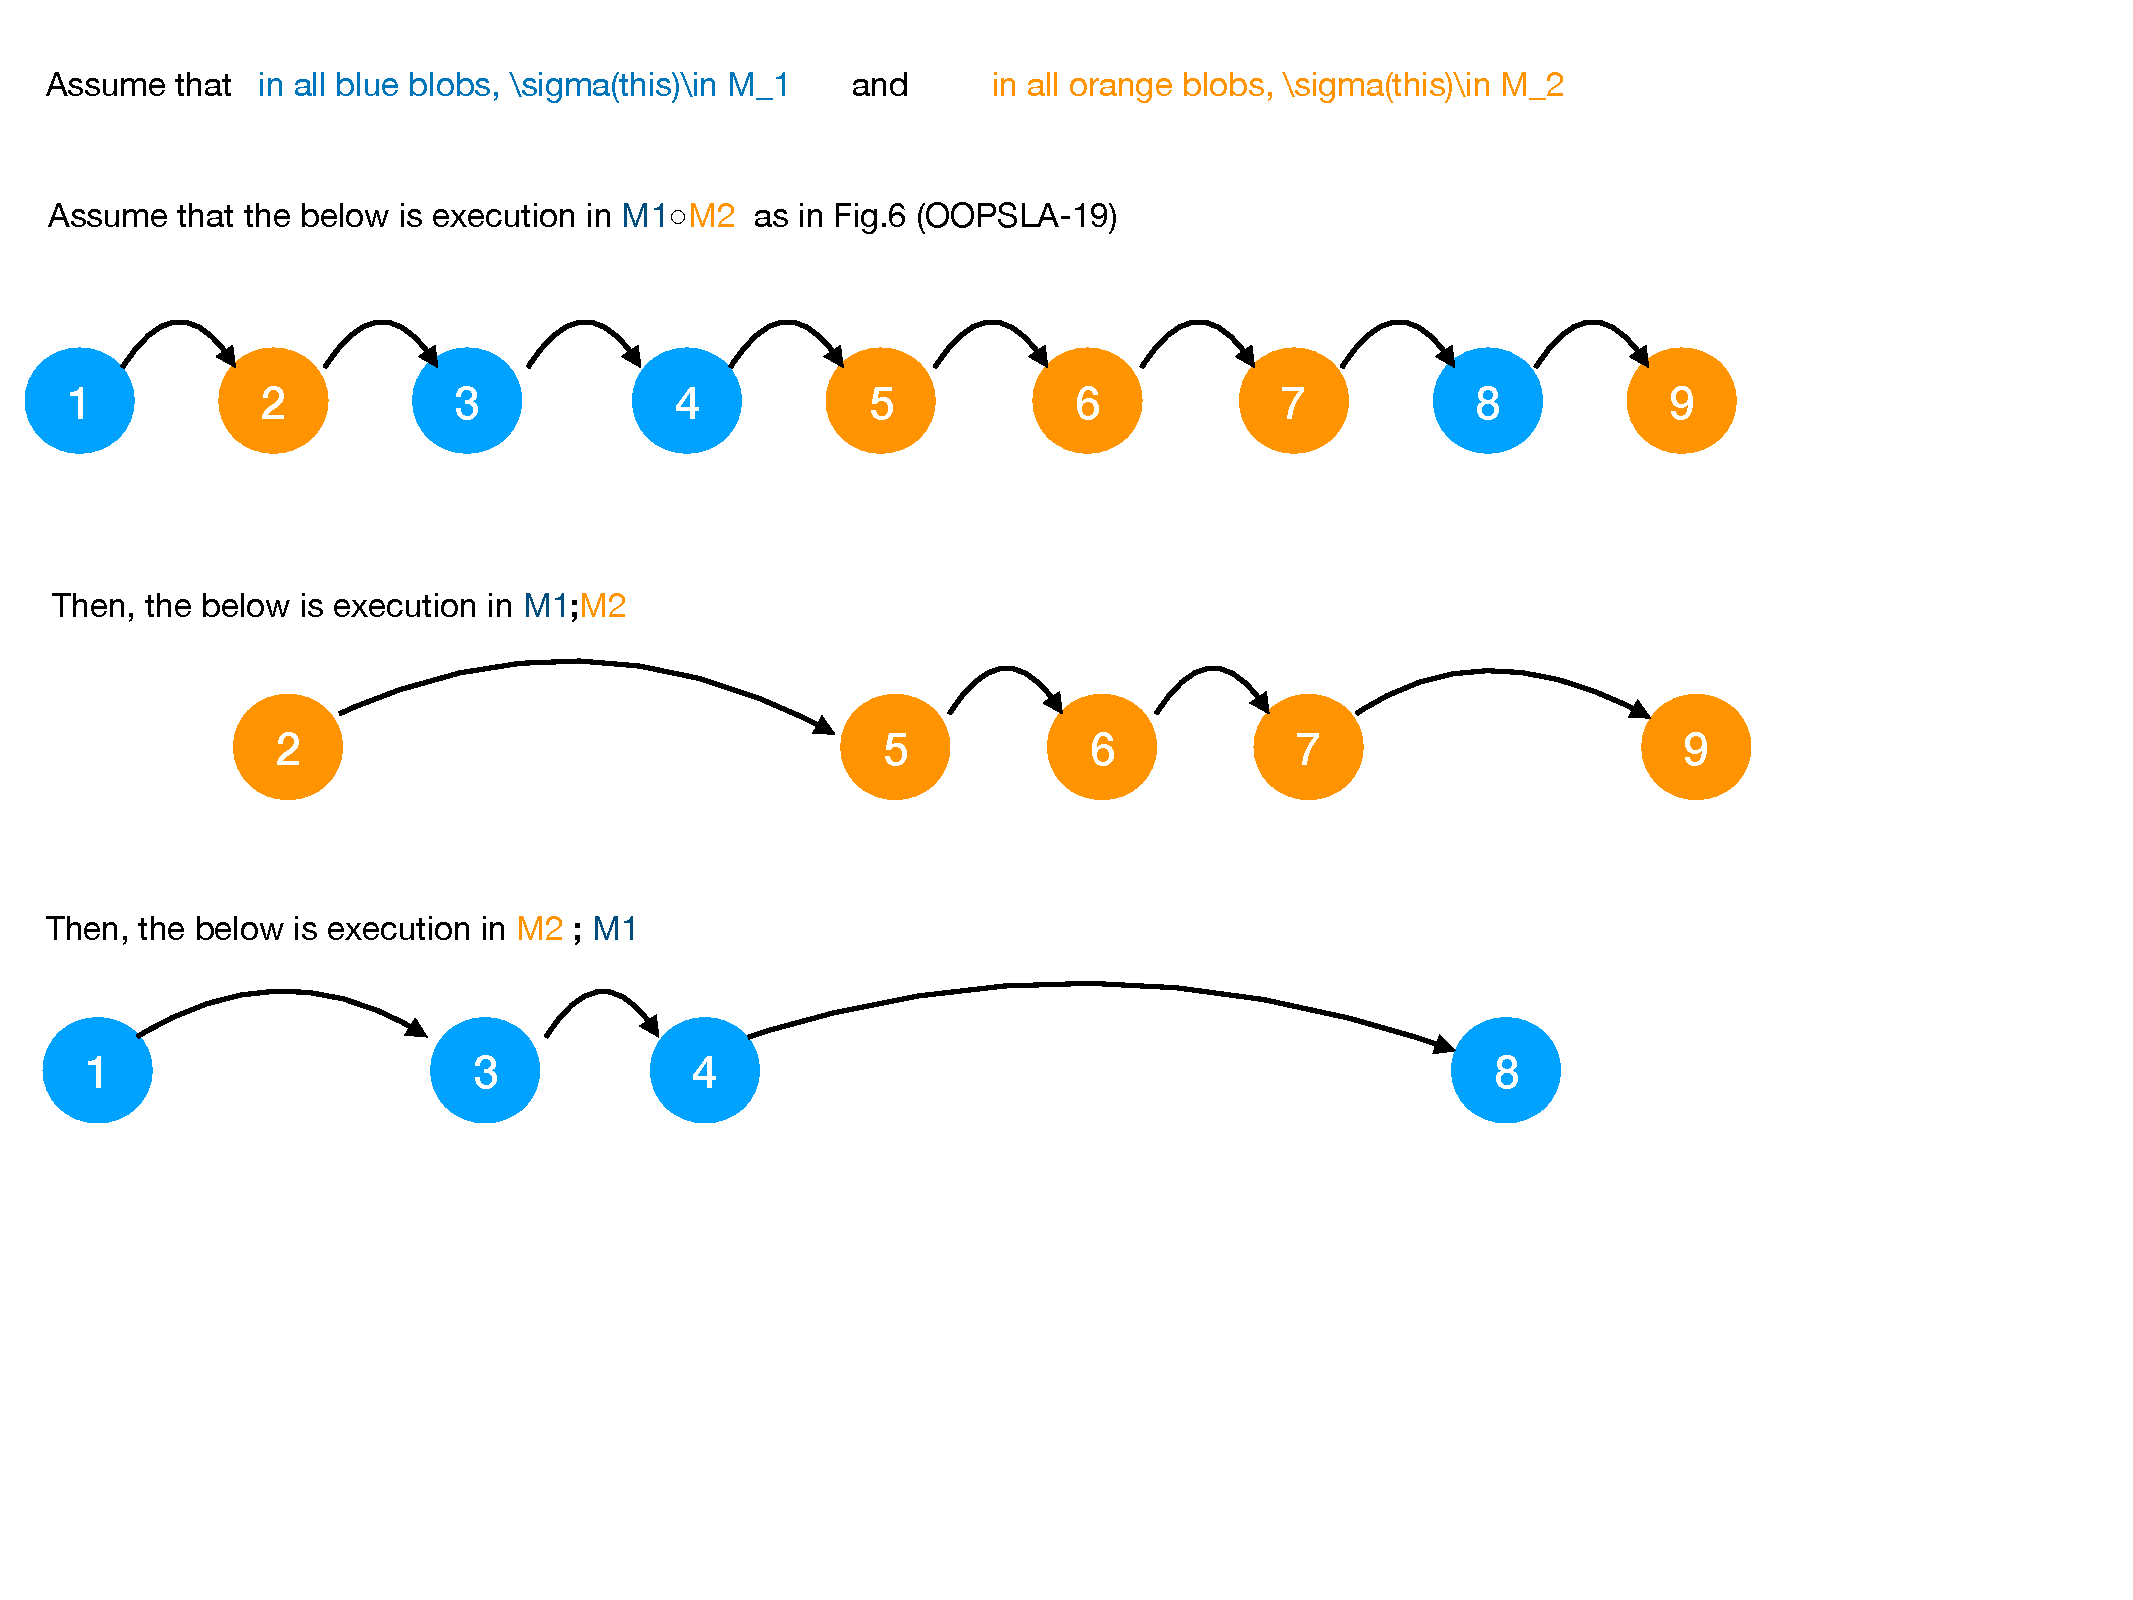
\includegraphics[width=\linewidth]{diagrams/VisibleStates.pdf}
     \end{center}
   \end{minipage}
   \end{center}
   \vspace*{-2.5mm}
   \caption{Two Module Execution
     (Def. \ref{def:execution:internal:external}). %
     %
     a) $\M_1 \link \M_2$ b) $\M_1 \mkpair \M_2$ c) $\M_2 \mkpair \M_1$}
   \label{fig:VisibleStates}
   \Description{Three rows of circles coloured blue and orange. In the top row are 9 circles labelled 1 through 9. Some are coloured blue, and some are coloured orange. In the next row, only the orange circles from the first are shown. In the final row, only the blue circles. Arrows connect successive circles in each row.}
 \end{figure}

Two-module execution  is related to % the concept of 
visible states
semantics \cite{MuellerPoetzsch-HeffterLeavens06} as they both filter configurations, with  the difference
that in visible states semantics % \sd{considers all intermediate configurations during execution, but
execution is unfiltered and  configurations are only filtered when it comes to the  consideration 
of class invariants\jm{,} while two-module execution filters execution.
%
The lemma below says  that linking is associative and commutative, and preserves   both one-module and two-module execution.

\begin{lemma}[Properties of linking]
\label{lemma:linking}
 For any modules $\M$,   $\M'$, $\M''$, and $\M'''$ and runtime configurations $\sigma$, and $\sigma'$ we have$:$
 \label{lemma:linking:properties}

 \begin{itemize}
     \item
     $(\M \link \M')\link \M''$ = $\M \link (\M' \link \M'')$  \hspace{1cm} and    \hspace{1cm}   $\M \link \M'$  = $\M' \link\M$.
      \item
      $\M, \sigma \leadsto \sigma'$, and $\M\link \M'$ is defined, \  \ \ \ \  implies\ \ \ \ \   $\M\link \M', \sigma \leadsto \sigma'$.
 \item
 $\M \mkpair \M', \sigma \leadsto \sigma'$   \  \ \ \ \  implies\ \ \ \ \  $(\M\link\M'') \mkpair (\M'\link\M''') ,\sigma \leadsto \sigma'$.  
  \end{itemize}

 \end{lemma}
 
 We can now answer the question as to which runtime configurations are pertinent when judging a module's
adherence to an assertion.
{\em Initial configurations} are those whose heap  have only one object, of class \prg{Object}, and whose stack have one frame, with arbitrary \jm{an} continuation.
{\em Arising} configurations are  those that can be reached by two-module execution, starting from a specific initial configuration to maintain temporal linearity.
 
\begin{definition}[Initial and Arising Configurations] defined as follows, using the semantics from Definition~\ref{def:runtimeentities}: \label{def:arise}

\begin{itemize}
     \item
   $\Initial {(\psi,\chi)}$, \ \ if \ \ $\psi$ consists of a single frame $\phi$ with $dom(\phi)=\{ \this \}$, and there exists  some address $\alpha$, such that \ \ \    $\interp {\this}{\phi}$=$\alpha$, and \ $dom(\chi)$=$\alpha$,\  and\  
    $\chi(\alpha)=(\prg{Object},\emptyset)$.
 \item
 $\Arising  {\M\mkpair\M', \sigma_0} \ = \ \{ \ \sigma \ \mid \ \Initial{\sigma_0}\ \wedge\ \M\mkpair\M', \sigma_0 \leadsto^* \sigma \ \ \} $
 \end{itemize}

\end{definition}
\jm{Arising configurations differ in their definition to that of previous work published at FASE 2020~\cite{FASE} in the usage of an initial configuration. In prior work
an arising configuration was defined as any configuration that might arise from {\em any} initial configuration. In linearizing Chainmail, we specify a specific initial 
configuration.}

\jm{We define a specialized form of two-module execution, \emph{constrained execution}.}
\begin{definition}[Constrained execution]  \label{def:reduction:constrained}
For any modules $\M$, $\M'$, and configurations $\sigma_1$, $\sigma_2$
\begin{itemize}
\item
$\M\mkpair \M',  \constrained \sigma_2$ 
\IFF
$\M\mkpair \M',  (\phi, \chi_1) \leadsto(\psi, \chi_2)$\\
$\strut ~ \hspace{1.4in} $ \hfill 
where
$\sigma_1 = (\phi \cdot \psi_1, \chi_1)$ and $\sigma_2 = (\psi \cdot \psi_1, \chi_2)$
and
\item
$\M\mkpair \M',  \sigma_1\constrained^* \sigma_2$ 
\IFF
$\M\mkpair \M',  (\phi, \chi_1) \leadsto^* (\psi, \chi_2)$\\
$\strut ~ \hspace{1.4in} $ \hfill 
where
$\sigma_1 = (\phi \cdot \psi_1, \chi_1)$ and $\sigma_2 = (\psi \cdot \psi_1, \chi_2)$
\end{itemize}
\end{definition}
\jm{Constrained execution (Definition \ref{def:reduction:constrained}) is a form of two-module execution
that is restricted to only those execution steps that arise from the top frame of the stack, and does not consider 
execution steps beyond a method return from the top frame.}

\jm{Constrained execution is a strict subset of two-module execution, and for all modules $\M$ and $\M'$, and configurations $\sigma_1$ and $\sigma_2$, 
if $\M\mkpair \M',  \sigma_1\constrained \sigma_2$ (or $\M\mkpair \M',  \sigma_1\constrained^* \sigma_2$), then 
it follows that $\M\mkpair \M',  \sigma_1 \leadsto \sigma_2$ (or $\M\mkpair \M',  \sigma_1\leadsto^* \sigma_2$). 
The reverse however is not true. Two-module execution does not imply constrained execution.
Since constrained execution does not consider any frames in the stack preceding the top frame of $\sigma_1$, 
$\sigma_2$ may only arise from the execution of the current method. For example, if the top frame of $\sigma_1$ 
is the result of a method call to some method $\prg{m}$, then constrained reduction is restricted to only intermediate 
configurations that arise from the evaluation of $\prg{m}$, and not beyond that.}

\jm{Constrained execution is used in the definition of satisfaction of the temporal operators $\Future{A}$ and $\Next{A}$ (defined in Section~\ref{sect:assertions}).
This restriction is necessary when considering the future, 
as \Chainmail is generally 
concerned with the current state of the program, and those states that 
might arise as a result. As an example, 
specification (2) of the introductory bank account example asserts that future changes to a bank account implies the current object has access to that account.
If the execution implied by future assertions were not constrained, this would not necessarily be true unless we inspected every frame in the stack to check access.
Further, future satisfaction of assertions beyond the present frame
would have no relation to the present scope. }

%\jm{Further, the use of constrained reduction is necessary in maintaining some expected properties of the temporal operators. 
%While the underlying language \LangOO is deterministic and linear in its reduction, and thus there is exactly one path from the initial configuration of the program to any 
%future configuration that must pass through the current configuration, this is not generally true of languages with potentially branching reduction. If
%reduction of \LangOO were non-linear, and satisfaction of $\Future{\A}$ (or $\Next{\A}$) were not defined with constrained reduction, 
%the satisfaction of $\A$ would not generally imply the satisfaction of $\Future{\Past{A}}$ as $\A$ would not necessarily be satisfied by every branch of the program leading to the future configuration.
%The inverse however does hold, i.e. due to the use of an initial configuration it always holds that satisfaction of $\A$ implies satisfaction of $\Past{\Future{\A}}.$}


\section{Assertions}
\label{sect:assertions}
\label{sub:SpecO}


Our assertions are  %\AssertLang, 
 standard  or  \emph{object-capability}. 
 Standard assertions assert properties of the values of fields, implication, quantification etc, as well as ghost fields  which represent user-defined predicates. 
The  object capability assertions express restrictions of  objects' eventual authority on other objects.

\begin{definition}
\label{def:assert:syntax}
%Expressions, $\re$, 
Assertions, $A$,  are defined as follows:

\label{f:chainmail-syntax}
$
\begin{syntax}
%\syntaxElement{\re}{}
%		{
%		\syntaxline
%				{\prg{true}}
%                                {{\alpha}}
%				{{x}}
%                                {\re.f}
%				{\re.f({\overline{\re}})}
%		\endsyntaxline
%		}
%\endSyntaxElement

\syntaxElement{A}{}
		{
		\syntaxline
				{{\re}}
				{{\re} : C}
				{\neg A}
				{A\ \wedge\ A}
				{\all{x:C}{A}}
				{\external{{\re}}}
 				{\protectedFrom{{\re}} {{\re}}} 
				 {\inside {{\re}}} 
		\endsyntaxline
		}
\endSyntaxElement\\
\end{syntax}
$
%In the above, we expect that
\footnote{Addresses in assertions % may contain addresses; 
as \eg  in  $\alpha.blnce > 700$, %. While addresses make little sense in user-written assertions, they are 
are useful when giving semantics to universal quantifiers 
\cf Def. \ref{def:chainmail-semantics}.(\ref{quant1}), {when the local map changes \eg upon call and return, and in general,} for scoped invariants, \cf Def. \ref{def:necessity-semantics}.}

\vspace{.1cm}

{$\fv(A)$ returns the free variables in $A$; for example, $\fv(a\!:\!Account \wedge \forall b:int.[a.\balance = b])$=$\{ a \}$.} 
% {{Moreover, $\fv(A)$ is defined in the obvious way to to return   the free variables in $A$; for example, $\fv(a\!:\!Account \wedge \forall b:int.[a.\balance = b])$=$\{ a \}$.}}

\end{definition}

\forget{
\noindent
\textbf{NOTES}  \notesep % Extended expressions, $\re$, and therefore also 
 Assertions  may contain addresses; \eg   $\alpha.bal > 700$. 
{While addresses make little sense in user-written assertions, they are useful when giving semantics to universal quantifiers 
\cf Def. \ref{def:chainmail-semantics}.(\ref{quant1}), {when the local map changes \eg upon call and return, and in general,} for two-state invariants, \cf Def. \ref{def:necessity-semantics}.(2).}
\notesep The syntax does  not distinguish between fields and ghost fields. For instance, $\prg{a}.\prg{\balance}$ may, in some modules (\eg in \ModA), be a field lookup, while in others (e.g. when the balance is defined though an entry in a lookup table) may involve executing a ghost function. 
% -  $\external {\re}$ is short for $\neg \internal {\re}$. We use these forms freely in the subsequent text without further definition.
% \footnoteSD{{\textbf{NOTE for us} It also allows assertions like $a1.passwd \neq a2.passwd$, whereas in the past we would have written as $\exists x,y.[\ a1.passwd=x \wedge  a2.passwd=y \wedge x\neq y\ ]$.}} \footnoteSD{{TODO compare with oopsla }}
}


\begin{definition}[Shorthands] 
{We write $\internal{\re}$ for $\neg (\external {\re})$}, and
$\extThis$. resp. {$\intThis$} for $\external{\prg{this}}$ resp. $\internal{\prg{this}}$. %, and $\re:\prg{intl}$ as short for $ \neg \external {\re}}$. 
Forms such as $A \rightarrow A'$,  $A \vee A'$, and $\exists x:C.A$  can be encoded.
%; we use these forms freely in the subsequent text.
% without further definition.
\end{definition}



\label{def:chainmail-semantics-all}
\label{dup:def:chainmail-semantics}
\noindent
Satisfaction  of Assertions by a module and a state is expressed  through \ $\satisfiesA{M}{\sigma}{{A}}$ \  and defined by cases on the shape of $A$, in definitions \ref{def:chainmail-semantics}  and 
 \ref{def:chainmail-protection}.
 {$M$} is used % might need to 
 to look up the definitions of ghost fields, and to find class definitions to determine whether an object is  external.
 
\footnoteSD{say why we split the def into three defs.} 
\noindent
%\textbf{NOTE}  
%{This is not surprising since the goal of this work is to ensure that external modules cannot break our (internal) module's assertions.}
%\footnoteSD{We need to have clarified internal module earlier.} 
%In most cases, satisfaction depends only on the state $\sigma$, but 
% in some cases it also depends on the module $M$: namely execution of extended expressions   
% -- c.f. Def. \ref{def:chainmail-semantics}, cases (\ref{cExpr}),  (\ref{cInternal}). %,  and (\ref{cExternal}) .

\subsection{Semantics of assertions % \AssertLang 
-- first part}
\label{sect:semantics:assert:standard}

To determine satisfaction of an expression, we    use the evaluation relation, $\eval{M}{\sigma}{e}{v}$,
which says that the expression $e$ evaluates
to value $v$ in the context of state $\sigma$ and module $M$.
As expressions in \LangOO may be recursively defined, their evaluation 
need not   % may not necessarily 
 terminate. Nevertheless, the logic of $A$ remains classical because recursion is restricted
to expressions. %, and not generally to assertions.
\footnoteSD{
The semantics of $\hookrightarrow$ {is} unsurprising 
(see {the appendices %of the full paper 
\cite{necessityFull}).}
We have taken this approach from \citeasnoun{FASE}, which also contains a mechanized Coq proof that assertions are classical \cite{coqFASE}. } %Fig.\ref{f:evaluation}).


\begin{definition}[Satisfaction 
of Assertions -- first part] 
\label{def:chainmail-semantics}
We define satisfaction of an assertion $A$ by a % program 
state $\sigma$ with 
 module $M$ as:
\begin{enumerate}
\item
\label{cExpr}
$\satisfiesA{M}{\sigma}{{\re}}\ \ \ \triangleq \ \ \   \eval{M}{\sigma}{{\re}}{\true}$
\item
\label{cClass}
$\satisfiesA{M}{\sigma}{{{\re}} : C}\ \ \ \triangleq \ \ \   \eval{M}{\sigma}{{\re}}{\alpha}\   \wedge \ \class{\alpha} {\sigma}= C$
\item
$\satisfiesA{M}{\sigma}{\neg A}\ \ \ \triangleq \ \ \   {M},{\sigma}\not\models{A}$
\item
$\satisfiesA{M}{\sigma}{A_1\ \wedge\ A_2}\ \ \ \triangleq \ \ \   \satisfiesA{M}{\sigma}{A_1} \   \wedge \ \satisfiesA{M}{\sigma}{A_2}$
%\item
%$\satisfiesA{M}{\sigma}{A_1\ \vee\ A_2}\ \ \ \triangleq \ \ \   \satisfiesA{M}{\sigma}{A_1}\   \vee \ \satisfiesA{M}{\sigma}{A_2}$
\item
\label{quant1}
$\satisfiesA{M}{\sigma}{\all{x:C}{A}} \ \ \ \triangleq \ \ \   
\forall \alpha.[\   \satisfiesA {M}{\sigma} {\alpha:C}  \ \Longrightarrow   \ \satisfiesA{M}{\sigma} {A[\alpha/x]} \ ] $

%\item
%\label{quant2}
%$\satisfiesA{M}{\sigma}{\ex{x:C}{A}}$ \ \ \ iff \ \ \  
% {$\exists \alpha.[\ \GRelevant \alpha \sigma \wedge  \satisfiesA {M}{\sigma} {\alpha:C}  \ \wedge \ \satisfiesA{M}{\sigma} {A[x/\alpha]}\ ]$.} 
%\item
%\label{cInternal}
%$\satisfiesA{M}{\sigma}{\internal{{\re}}}$ \ \ \ iff \ \ \   $\satisfiesA{M}{\sigma}{{{\re}} : C} \ \wedge\ \ C \in M$
\item
\label{cExternal}
$\satisfiesA{M}{\sigma}{\external{{\re}}} \ \ \ \triangleq \ \ \  \exists C.[\ \satisfiesA{M}{\sigma}{{{\re}} : C} \ \wedge \ C \notin M \ ]$
\end{enumerate}
\end{definition}

 
Note that while execution takes place in the context of one or more modules, $\Mtwo$, satisfaction of assertions considers \emph{exactly one} module  $M$ -- the internal module. 
{$M$} is used  to look up the definitions of ghost fields, and to % find class definitions to 
 determine whether objects are  external.

\subsection{Semantics of Assertions - second part}  

\label{sect:protect}
% Long motivation.
% However the motivation from sect 2 shoud be sufficient
%In the object capabilities model \cite{MillerPhD}, \emph{access} to a capability (called a \emph{permission} in \cite{MillerPhD}
% is a necessary precondition  for producing a given effect;  as expressed by the principle that ``authority (to cause an effect) implies eventual permission'' \cite{permissionAuthority}.
%As   in \S \ref{sec:shop}, and also \cite{OOPSLA22}, if no external object has eventual access for a given capability, then the corresponding effect cannot occur.
% Specifically,  we say that $o$ \emph{has eventual access to} $o'$, to mean  that $o$ either currently has or will acquire direct access to $o'$ in the future \cite{permissionAuthority}.
%
%
%
%Given this, it becomes essential to determine whether eventual access exists in a given state. 
%Unfortunately, this determination is undecidable, as it depends not only on the current object graph but also on the program code being executed.
%
%In this work, we over-approximate lack of eventual access through a combination of two properties: one pertaining to the state, and the other to the internal code. 
%The  property pertaining to the state is $\satisfiesA{M}{\sigma} {\inside {\alpha}}$, \ie that   $\alpha$ is \emph{protected},
%\ie that   {no locally reachable external objects have direct access to $o$.}
%% on any path from a locally reachable object to $o$, the penultimate object  is internal. 
%The  property pertaining to the program is that it preserves the protection of   $o$.
%%
%We can see that if $o$ is protected and the internal code preserves its protection, then no external object can gain eventual access to $o$.

In \S \ref{sect:approach:protection} we % discussed the importance of a guarantee that there will be no external access to a capability, and how this can be modelled 
introduced protection -- we will now formalize this concept. % in Def. \ref{def:chainmail-protection-from}.

 An object is protected from another object, $\protectedFrom{{\alpha}} {{\alpha_{o}}}$, if 
the two objects are not equal, and no external object reachable from $a_o$ has a field pointing to  $\alpha$.
This ensures  that any path leading from $\alpha_o$ to $\alpha$ also leads through an internal object.
 

An object is protected,  $\inside{{\alpha}}$,  if no external object reachable from any of the current frame's arguments has a field pointing to $\alpha$, and if the receiver is external, then   $\alpha$ is not the value of any parameter.  
This  ensures that no external objects reachable from the current receiver or arguments have direct access to $\alpha$ -- such direct access
 is either through a field, or by virtue of the receiver having access to all the arguments.
 


 
\begin{definition}[Satisfaction 
of Assertions  -- Protection] 
\label{def:chainmail-protection-from}
\label{sect:semantics:assert:prtFrom}
 \label{def:chainmail-protection}
-- continuing definitions in \ref{def:chainmail-semantics}:
\begin{enumerate}
\item
\label{cProtected}
 $\satisfiesA{M}{\sigma}{\protectedFrom{{\alpha}} {{\alpha_{o}}}}   \ \ \ \triangleq $ 
  \begin{enumerate}
 \item
$\alpha\neq \alpha_0$,
 % \ \ \ \  and 
 \item
$\forall \alpha'.\forall f.[\ \alpha' \in {\Relevant {\alpha_o} {\sigma}} \wedge\   \satisfiesA{M}{\sigma}{\external {\alpha'}} 
\ \ \Longrightarrow \ \  
  \interpret {\sigma} {\alpha_o.f} \neq \alpha     \ ] $.
\end{enumerate}
\item
\label{sect:semantics:assert:prt}
$\satisfiesA{M}{\sigma} {\inside {\alpha}}  \ \ \ \triangleq \ \ \   $
 \begin{enumerate}
\item
 $\satisfiesA{M}{\sigma}{\extThis}\ \ \Longrightarrow\ \ \forall x\!\in\! \sigma.\ \satisfiesA{M}{\sigma}{x\neq \alpha}$,
 \item
$\forall \alpha'.\forall f.[\ \alpha' \in {\LRelevantO {\sigma}} \wedge\   \satisfiesA{M}{\sigma}{\external {\alpha'}} 
\ \ \Longrightarrow \ \  
  \interpret {\sigma} {\alpha_o.f} \neq \alpha     \ ] $.
  \end{enumerate}
\end{enumerate}
Moreover,  \\
$\strut \ \ \ \ \ \  (3) \ \  \satisfiesA{M}{\sigma}{\protectedFrom{{\re}} {{\re_{o}}}}$ $ \triangleq$
$\exists \alpha, \alpha_{o}. [\  \eval{M}{\sigma}{{\re}}{\alpha}\ \wedge\ \eval{M}{\sigma}{{\re_0}}{\alpha_0} \  \wedge \ 
  \satisfiesA{M}{\sigma}{\protectedFrom{{\alpha}} {{\alpha_{o}}}}\   ]$, \\
  $\strut \ \ \ \ \ \ (4) \ \ \satisfiesA{M}{\sigma}{\inside{\re}}$  $\triangleq$
 $\exists \alpha. [\   \eval{M}{\sigma}{{\re}}{\alpha}\ \wedge \   \satisfiesA{M}{\sigma}{\inside{\alpha}} \  ]$. 

 \end{definition} 
 
 We illustrate "protected" and "protected from" in Fig.  \ref{fig:ProtectedBoth} in \S \ref{s:outline},
and    Fig.  \ref{fig:ProtectedFrom} in App. \ref{appendix:assertions}.
%
In general,  $\protectedFrom{{\alpha}} {{\alpha_{o}}}$ ensures that $\alpha_o$ will get access to $\alpha$ only if another object 
 % an internal object 
 grants that access.
Similarly, $\inside \alpha$ ensures that during execution of the current method, no external object will get direct access to $\alpha$ unless some internal object grants that access.
\footnote{This is in line with the motto "only connectivity begets connectivity" from \cite{MillerPhD}.}
Thus, protection together with protection preservation  (\ie no internal object gives access) guarantee
%are sufficient but not necessary conditions for 
lack of eventual external access.  

 
\footnoteSD{JAMES' comment: If is possible that ``we'' do not know the complete heap (eg we only know about the green stuff.) how do we know whether an object is protected. The answer is that we do not know that it is protected, but we do know that our code guarnartees poreservation of protectedness.
}  
 
 \subsubsection*{Discussion} 
Lack of  eventual 
direct access is a central concept in the verification of code with calls to and callbacks  from untrusted code.
% ARGHHH a joke citatiion? \cite{praiseYou}.   
%Unmediated access is essentially \citet{MillerPhD}'s permission: that we have a ``first
%class'' reference to the capability; that we can call any 
%method in the capability's public interface; that we can
%store or save or present the capability to any other
%object to which we've been introduced
%%\footnote{``nobody can ever be introduced in a ball-room''}
It has already been over-approximated in several different ways, \eg
2nd-class \cite{rompf-second-class-oopsla2016,rompf-dont-pop-second-class-ecoop2022}
or borrowed (``2nd-hand'') references
\cite{boyland-promises-icse1998,boyland-aliasburying-spe2001},
 textual modules \cite{OOPSLA22},
information flow \cite{ddd}, runtime
checks \cite{secure-io-fstar-popl2024},
abstract data type exports \cite{vmsl-pldi2023},
  separation-based invariants 
Iris \cite{iris-wasm-pldi2023,cerise-jacm2024},
-- more in  \S~\ref{sect:related}.
In general, protection is applicable in more situations (i.e.\ is less
restrictive) than most of these approaches,
 although more restrictive than the ideal ``lack of eventual access''. 
\footnoteSD{ HER WHAT IT USED TO SAY: the contrapositive ideal that lack of eventual access ensures
lack of effect. Note that ``cannot get direct access'' does not generally imply ``is protected''. 
}





\noindent
\begin{flushleft}
\begin{tabular}{@{}lr@{}}
  \begin{minipage}{.85\textwidth}
   {An alternative definition might consider $\alpha$ as protected from $\alpha_o$, 
if   any path from $\alpha_o$ to $\alpha$ goes through at least one internal object.
With this definition, $o_4$ would be protected from $o_1$ in the heap shown here.
However,  $o_1$ can make a call to $o_2$, and  this call could  return $o_3$. 
Once $o_1$ has direct access to $o_3$, it can also get direct access to $o_4$. 
The example justifies our current definition.  
}
\end{minipage}
& 
\begin{minipage}{.18\textwidth}
\resizebox{2cm}{!}{
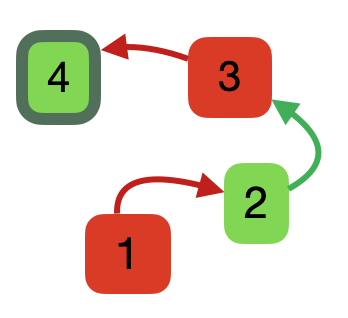
\includegraphics[width=\linewidth]{diagrams/altDef.png}
} 
\end{minipage}
\end{tabular}
\end{flushleft}


%Protection --- \sdN{objects to which external objects may not get %which objects can get 
%unmediated access} % to which other objects 
%---  is  a crucial concept: It enables
%the verification code in the open world, % even in the presence of
%with calls to and callbacks 
%from untrusted code.
%% ARGHHH a joke citatiion? \cite{praiseYou}.   
%Unmediated access is essentially \citet{MillerPhD}'s permission: that we have a ``first
%class'' reference to the capability; that we can call any 
%method in the capability's public interface; that we can
%store or save or present the capability to any other
%object to which we've been introduced
%%\footnote{``nobody can ever be introduced in a ball-room''}
%(compare
%2nd-class \cite{rompf-second-class-oopsla2016,rompf-dont-pop-second-class-ecoop2022}
%or borrowed (``2nd-hand'') references
%\cite{boyland-promises-icse1998,boyland-aliasburying-spe2001}
%which are restricted in some way),
%without reference to some owning class or defining module.
%We discuss alternative designs,
%ranging from overly simplistic textual modules \cite{OOPSLA22},
%information flow \cite{ddd}, runtime
%checks \cite{secure-io-fstar-popl2024},
%abstract data type exports \cite{vmsl-pldi2023},
%to automated separation-based invariants in
%Iris \cite{iris-wasm-pldi2023,cerise-jacm2024},
%in section~\ref{sect:related}.
%In general, protection is applicable in more situations (i.e.\ is less
%restrictive) than most of these approaches,
% \sdN{although more restrictive than the ideal "lack of eventual permission"}. 
%\footnoteSD{ HER WHAT IT USED TO SAY:
%the contrapositive ideal that lack of eventual permission ensures
%lack of effect. Note that ``cannot get direct access'' does not generally imply ``is
%protected''


 


\section{Examples}
\label{sect:example}

In this section we look at a couple of further examples from the
literature where a holistic specification would provide obvious
benefits in ensuring robustness.

\subsection{Attenuating the DOM}
\label{sect:example:DOM}
\input{ExampleDOM}

\subsection{Authorizing the ERC20}
\label{sect:example:ERC20}
\sd{ 
 ERC20~\cite{ERC20} is a widely used token standard which describes the 
 basic functionality expected by any    Ethereum-based token contract. 
 It issues and keeps track of participants' tokens, and supports the  transfer
 of tokens between participants. 
%
%
%An important question, therefore, is to identify the precise circumstances under which a transfer of tokens may take place.
%The answer is that 
Transfer of tokens 
 can   take place only provided that  there were sufficient tokens in the
 owner's account, and that
 the transfer was instigated by the owner, or by somebody authorized
 by the owner.

We specify this in \Chainmail as follows:
A decrease in  a participant's \prg{balance} 
%(\ie  $\prg{e}.\prg{balance}=...\, \wedge\, \Next{\prg{e}.\prg{balance}=...}$)
can only be caused by a transfer instigated by the 
account holder themselves\\ (\ie $\Calls {\prg{p}} {\prg{transfer}} {...} {...}$), or by
an authorized transfer instigated by another participant $\prg{p}''$  (\ie $\Calls {\prg{p}''} {{\prg{transferFrom}} } {..} {..}$) who 
has authority for more than the tokens spent (\ie  $\prg{e}.\prg{allowed}(\prg{p},\prg{p}'')\geq \prg{m}$)
 
\vspace{.15cm}
\noindent
% \strut \hspace{0.3cm} 
$\forall \prg{e}:\prg{ERC20}.\forall \prg{p}:\prg{Object}.\forall \prg{m},\prg{m}':\prg{Nat}.$\\
\strut \hspace{0.3cm} $[\ \ \prg{e}.\prg{balance(p)}=\prg{m}+\prg{m'}\ \wedge \ \Next{\prg{e}.\prg{balance(p)}=\prg{m}'}$ \\ %.\forall\prg{m}:\prg{Nat}.$\\
\strut \hspace{0.4cm} \ \ \ $\longrightarrow$\\
\strut \hspace{0.4cm} \ \ \ $\exists \prg{p}',\prg{p}'':\prg{Object}.$ \\
\strut \hspace{0.4cm} \ \ \  $[\ \  \Calls{\prg{p}} {\prg{transfer}}  {\prg{e}}  {\prg{p}',\prg{m}} \  \  \ \vee\, $\\
\strut \hspace{0.4cm} \ \ \   $\ \ \ \ \prg{e}.\prg{allowed}(\prg{p},\prg{p}'')\geq \prg{m} \ \wedge \ \Calls{\prg{p}''} {\prg{transferFrom}}  {\prg{e}}  {\prg{p}',\prg{m}}\       \  ]$\\
\strut \hspace{0.3cm} $] $
\vspace{.15cm}

\noindent
That is to say: if next configuration witnesses a decrease of \prg{p}'s balance by
 $\prg{m}$, then the current configuration was a call of \prg{transfer} instigated by
 \prg{p}, or  a call of \prg{transferFrom} instigated by somebody authorized by \prg{p}.
 The term $\prg{e}.\prg{allowed}(\prg{p},\prg{p}'')$,  means that the
ERC20 variable \prg{e} holds a field called \prg{allowed}   which maps pairs of participants to numbers; such
mappings are supported in Solidity\cite{Solidity}.
 
We now define what it means for $\prg{p}'$ to be authorized  to  spend 
up to \prg{m} tokens on  $\prg{p}$'s behalf: At some point in the
past,  \prg{p} gave authority to $\prg{p}'$  to spend   \prg{m}
plus the sum of  tokens
spent so far by $\prg{p}' $ on the behalf of \prg{p}. 

 
\vspace{.15cm}
\noindent
 $\forall \prg{e}:\prg{ERC20}.\forall \prg{p},\prg{p'}:\prg{Object}.\forall \prg{m}:\prg{Nat}.$\\
\strut \hspace{0.3cm} $[\ \ \prg{e}.\prg{allowed}(\prg{p},\prg{p}')=\prg{m} $\\
\strut \hspace{0.4cm} \ \ \ $\longrightarrow$\\
\strut \hspace{0.4cm} \ \ \  
     $\PrevId\langle\ \  \Calls{\prg{p}}  {\prg{approve}}  {\prg{e}} {\prg{p}',\prg{m}} $\\
      \strut \hspace{1.7cm} \ $\vee $\\
\strut \hspace{1.7cm} \  
     $    \prg{e}.\prg{allowed}(\prg{p},\prg{p}')=\prg{m}   
        \  \wedge\ $\\
\strut \hspace{1.5cm} \ \ \ \ \          
$  \neg   (\, {\Calls{\prg{p}'} {\prg{transferFrom}} {\prg{e}} {\prg{p},\_}   } \, \vee \, {\Calls{\prg{p}} {\prg{approve}} {\prg{e}} {\prg{p},\_} } \, ) $\\
      \strut \hspace{1.7cm}\  $\vee $\\
\strut \hspace{1.7cm}   \  $ \exists \prg{p}'':\prg{Object}.\exists\prg{m'}:\prg{Nat}.$\\
 \strut \hspace{1.7cm}\  $[\   
  \prg{e}.\prg{allowed}(\prg{p},\prg{p}')=\prg{m}+\prg{m}'  \, \wedge\,   {\Calls{\prg{p}'} {\prg{transferFrom}} {\prg{e}} {\prg{p}'',\prg{m}'}  }   ]$\\
\strut \hspace{0.4cm} \ \ \  \ \ \  \ \ \ \ \ $\rangle $\\
\strut \hspace{0.3cm} $]$
\vspace{.15cm}
 
In more detail\  $\prg{p}'$ is allowed to spend 
up to \prg{m} tokens on their behalf of $\prg{p}$, if in the   previous step either a)
 \prg{p} made the call \prg{approve} on \prg{e} 
with arguments $\prg{p}'$ and \prg{m}, or b)  
$\prg{p}'$ was allowed to spend  up to \prg{m} tokens for $\prg{p}$
and did not transfer any of \prg{p}'s tokens, nor did \prg{p} issue a fresh authorization,
or c) \prg{p} was authorized for $\prg{m}+\prg{m}'$ and spent $\prg{m}'$. 
  
  \vspace{.1cm}
 
 Thus, the holistic specification gives to account holders an
 "authorization-guarantee": their balance cannot decrease unless they
 themselves, or somebody they had authorized, instigates a transfer of
 tokens. Moreover, authorization is {\em not} transitive: only the
 account holder can authorise some other party to transfer funds from
 their account: authorisation to spend from an account does not confer
 the ability to authorise yet more others to spend also.
 
% \paragraph{Comparison with Traditional Specifications}
 
 With traditional  specifications, to obtain the "authorization-guarantee", 
one would need to inspect the pre- and post- conditions of {\em all} the functions
in the contract, and determine which of the functions decrease balances, and which of the functions 
 affect authorizations.
 In the case of the \prg{ERC20}, one would have to inspect all eight such specifications
 (given in appendix \ref{ERC20:appendix}), 
 where only five are relevant to the question at hand.
 In the general case, \eg the DAO, the number of   functions which are unrelated
 to the question at hand can be very large.
  
More importantly, with traditional  specifications, nothing stops the next release of the contract to add, 
\eg, a method which allows participants to share their authority, and thus
violate the "authorization-guarantee", or even a super-user from skimming 0.1\% from each of the accounts.

}


\subsection{Defending the DAO}

\sd{We specidy the DAO in appendix \ref{Dao:appendix}}
%The DAO  {(Decentralised Autonomous Organisation)}~\cite{Dao}  is a famous Ethereum contract  which aims to support
collective management of funds,  and to place power directly in the
hands of the owners of the DAO
rather than delegate it to directors.
Unfortunately, the DAO was not robust:
a re-entrancy bug   exploited in June 2016 led  to a loss of   \$50M, and
a hard-fork in the  chain ~\cite{DaoBug}.
%
%In a similar style as that  of the ERC20 spec earlier,
%We can give a \Chainmail~specification
With holistic specifications  we can  write a succinct requirement that a
DAO contract should always be able to repay any owner's money.
Any contract which satisfies such a holistic specification cannot demonstrate the DAO bug.
 
Our specification consists of \jm[]{two} requirements.
First, that the DAO always holds at least as 
much money as any owner's balance\jm[I added this to make it clear that we don't need to talk about all owners]{, and thus is always able to repay any owner}.
%  \james{ALL owners? or does that follow?} 
To express this we use 
the field \prg{balances} which is a mapping from participant's addresses to 
numbers. Such mapping-valued fields exist in Solidity, but 
\jm{in \Chainmail it could be a real field or a ghost field.}
%they could
%also be taken to be ghost fields~\cite{ghost}.
  
\vspace{.1cm}

\noindent
 \strut \hspace{0.5cm} $\forall \prg{d}:\prg{DAO}.\forall \prg{p}:\prg{Any}.\forall\prg{m}:\prg{Nat}.$\\
\strut \hspace{0.5cm} $[\ \ \prg{d.balances(p)}=\prg{m}  \ \ \  \longrightarrow  \ \ \ \prg{d}.\prg{ether}\geq \prg{m} \ \ ] $
  \jm[should spec 2 be done in classical spec? extend chainmail?]{}

 

%\kjx{combined defn ensuring enough eth at the time repayment is made:\\
%\noindent
% \strut \hspace{0.5cm} $\forall \prg{d}:\prg{DAO}.\forall \prg{p}:\prg{Any}.\forall\prg{m}:\prg{Nat}.$\\
%\strut \hspace{0.5cm} $[\ \ \prg{d.balance(p)}=\prg{m}
% \ \wedge \ \Calls{\prg{p}}{\prg{repay}}{\prg{d}}{\_}  $\\
% $\strut \hspace{5.5cm}   \ \ \  \longrightarrow  \ \ \  \Future{\Calls{\prg{d}}{\prg{send}}{\prg{p}}{\prg{m}}
% \wedge \prg{d}.\prg{ether}\geq \prg{m}}\ \ ] $
%\vspace{.1cm}
%}
%
%\kjx{negative example for talk, upping funds not calling send:\\
%\noindent
% \strut \hspace{0.5cm} $\forall \prg{d}:\prg{DAO}.\forall \prg{p}:\prg{Any}.\forall\prg{m}:\prg{Nat}.$\\
%\strut \hspace{0.5cm} $\ \ \Calls{\prg{d}}{\prg{send}}{\prg{p}}{\prg{m}}
% \strut \ \ \  \longrightarrow  \ \ \  \prg{d}.\prg{ether}\geq \prg{m}$\\
% % SD thinks the last  \longrightarrow sgould be wedge
%  $\strut \ \ \  \longrightarrow  \ \ \  \prg{p.funds}
%  = \Prev{\prg{p.funds}} + \prg{m}$
%\vspace{.1cm}
%}


\noindent
\sd{\jm{Second}, that the balance of an owner is a function of its balance in the previous step,
or the result of it joining the DAO, or asking to be repaid \etc.}
 
\noindent
$\strut \hspace{0.5cm} \forall \prg{d}:\prg{DAO}.\forall \prg{p}.\forall:\prg{m}:\prg{Nat}.$\\
$\strut \hspace{0.5cm} [ \ \ \  \prg{d.Balance(p)}=\prg{m} \ \ \  \longrightarrow   
 \ \  \ \ 
  [ \  \ \Prev{\Calls{\prg{p}}{\prg{repay}}{\prg{d}}{\_}}\, \wedge\, \prg{m}=\prg{0} \ \ \ \ \vee $\\
$\strut \hspace{5.7cm}      
\Prev{\Calls{\prg{p}}{\prg{join}}{\prg{d}}{\prg{m}}}  \ \ \ \ \vee   $\\
 $\strut \hspace{5.7cm}  ... \  ]$ \\
%                         
%                         $ \left\{
%                            \begin{array}{ll}
%                             \prg{0}, & \hbox{if}\ Prev(Call(\prg{p},\prg{d.repay(),\_})    \\
%                             \vee
%                             \\
%                             \prg{m},  & \hbox{if}\  Prev(Call(\prg{p},\prg{d.join(),m}))   \\
%                             ..., & ...
%                           \end{array}
%                         \right.    $\\
$\strut \hspace{0.5cm} ] $


\jm[reworded]{In order to reflect the financing and repayments of proposals, more cases are needed, however they can be expressed with the concepts described so far.}
 

\jm[added break before paragraph]{}
The requirement that \prg{d} holds at least \prg{m} ether precludes the DAO bug,
in the sense that  any contract satisfying that spec cannot exhibit  the  bug:   a contract
which satisfies the spec  is guaranteed to always have enough money to satisfy all \prg{repay} requests.
This guarantee  holds, regardless of how many functions there are in the DAO.
In contrast, to preclude the DAO  bug with a classical spec, one would need to write a spec for each of the
DAO functions (currently 19), a spec for each function of the auxiliary contracts used by the DAO,
and then study their emergent  behaviour.

These 19 DAO functions   have several different concerns:
who may vote   for a proposal, who is eligible to submit a proposal,
how long the consultation period is for deliberating a proposal, what
is the quorum, how to chose curators, what is the value of a token,
Of these groups of functions, only  a handful affect the balance of a
participant. Holistic specifications allow us to concentrate on aspect of DAO's behaviour across \emph{all} its functions.

\jm[]{
\noindent
It is notable that Chainmail is only able to specify how client code interacts
with the DAO, and not how the DAO interacts with client code.
A third specification might say that when an owner asks to be repaid, she is sent all her money.\\
\vspace{.1cm}
\noindent
 \strut \hspace{0.5cm} $\forall \prg{d}:\prg{DAO}.\forall \prg{p}:\prg{Any}.\forall\prg{m}:\prg{Nat}.$\\
\strut \hspace{0.5cm} $[\ \ \prg{d.balance(p)}=\prg{m}
 \ \wedge \ \Calls{\prg{p}}{\prg{repay}}{\prg{d}}{\_}  $\\
 $\strut \hspace{5.5cm}   \ \ \  \longrightarrow  \ \ \  \Future{\Calls{\prg{d}}{\prg{send}}{\prg{p}}{\prg{m}}}\ \ ] $  
\vspace{.1cm}\\
The above specification is not legal Chainmail, as \Calls{\prg{d}}{\prg{send}}{\prg{p}}{\prg{m}}
specifies a method call made by internal DAO code. 
This example specification indicates that Chainmail might benefit from
the ability to specify calls to external code.
}


\section{Discussion}
\label{sect:discussion} 

\paragraph{Specification Language}

%\kjx{this section is new, but James didn't really know what Sophia wanted.}

The key to writing and using holistic specifications is to capture the
implicit assumptions underlying the design of the system we are
specifying.  The design principle animating the design of \Chainmail\
is to make writing holistic specifications as straightforward as
possible.

This is why we support bi-directional temporal operators (``will'',
``was'' etc) rather than just one temporal direction. Some assertions
are easier to express looking forwards (if a vending machine takes a
coin it will eventually dispense a chocolate bar) while other
assertions \jm{are} easier to express looking backwards (if a vending
machine dispenses a chocolate bar, it has already accepted the coin
to pay for it).

Similarly, in an imperative setting, the question of whether a change can
occur at all is at least as important as the precise details of the
change. This is why we support the ``changes'' operator in \Chainmail;
to enable specifications to capture that notion directly, rather than
e.g.\ expressing explicit differences in values between pre- and post-
states.

For modelling the open world, the interactions between the external
and internal modules are essential.
\sdf{Therefore in assertions we distinguish the internal from the external module,
$\M\mkpair \M', ... \models \A$,
and we consider that an internal module 
$\M$ satisfies an invariant $\A$, when all reachable states which lie outside $\M$ satisfy $\A$; 
for this, we introduced two-module execution $\M\mkpair \M',\sigma \leadsto \sigma'$.
 }
%\kjx{doesn't know what more to say here someone else can fill it in} 
We \sdf{also} included predicates $\External {\_}$ and     $\Internal {\_}$  to   %be able to state explicitly 
\sdf{state} % state is enough
which side of the boundary between modules \sdf{an object is}.
% SD chopped; nothing crosses, I think  and what can cross that boundary.


\sdf{A major aspect of the design of  \Chainmail was the treatment of recursion:
We wanted to support the writing of   predicates in
a natural way, and therefore allow for unrestricted recursion. However, unbounded recursion opens the possibility of infinite expansion, and
this, in turn may introduce contradictions into the logic.
Our solution is based on a two-tier approach: We distinguish between expressions and assertions,
where expressions may appear in assertions, and where 
we allow unrestricted recursion in expressions.
Thus we do not support user-defined, recursive predicates, but do allow
\jm{user}-defined recursive functions in the form of ghost fields.
An assertion which consists of an expression has the value of that
expression, if the  expression has a  finite expansion returning  that a value,
and otherwise is $\false.$ 
Thus, expressions are not classical, but assertions are. 
For example, it does not hold for all boolean expressions $e$ that $\prg{if}\ \ \prg{e}\  \prg{then} \ \true \ \prg{else} \ \false$ returns $\true$, but it does hold  for all assertions $\A$ that $\A \vee \neg \A$ holds.
}


The issues we have had to deal with are those related to space in
various ways: ``access'', ``in'', and ``external''.  One object
referring to another appears simple enough on the surface, but causes
significant problems in an open world setting. In \Chainmail, these
problems appear with universal quantification on the source of a
reference: ``in'' enables us to bound these quantifications.



\paragraph{Underlying Language}

%\kjx{pulled in from earlier version}

For our underlying language, we have chosen an object-oriented, class based language,
%\sd{but we  expect that the ideas} will also be
%applicable to other kinds of languages (object-oriented or
%otherwise).
%% \sd{We  could, \eg} extend our work to prototype-based programming
%% by creating an (anonymous) class to reify each
%% prototype \cite{graceClasses}. 
%
We have chosen to use a dynamically typed language because many of the
problems we hope to address are written in these
languages: web apps and mashups in Javascript; backends in Ruby\jm{, Python}, or
PHP.  We expect that supporting types would make the problem easier,
not harder, but at the cost of significantly increasing the complexity
of the trusted computing base that we assume will run our programs. In
an open world, without some level of assurance (e.g. proof-carrying
code) about the trustworthiness of type information: unfounded
assumptions about types can give rise to new vulnerabilities that
attackers can exploit \cite{pickles}. We don't address inheritance, as although it provides helpful abstractions, it doesn't change the fundamental problems, since in a dynamically-typed language it can be encoded through duplicating functionality in different classes.

As a specification language,
individual \Chainmail assertions can be combined or reused without any
inheritance mechanism: the semantics are simply that all
the \Chainmail\ assertions are expected to hold at all the points of
execution that they constrain.  \LangOO\ does not contain inheritance
simply because it is not necessary to demonstrate specifications of
robustness: whether an \LangOO class is defined in one place, or
whether it is split into many multiply-inherited superclasses, traits,
default methods in interfaces or protocols, etc.\ is irrelevant,
provided we can model the resulting (flattened) behaviour of such a
composition as a single logical \LangOO\ class.

\jm{
\paragraph{Linear Temporal Logic}
Earlier work on \Chainmail~\cite{FASE} featured a non-linear temporal logic
where all possible executions through a program were considered simultaneously.
In considering the past, all possible branches stemming from all possible 
initial configurations that might have preceded the current configuration
were considered. Similarly, when considering the future, all possible branches 
that might arise from the current configuration were considered. In this paper we
constrain satisfaction of temporal operators to consider only a single execution 
path at a time. This is done by (a) designing the underlying language such that its
execution is deterministic, thereby ensuring the future is linear, and  (b) considering 
satisfaction in relation to only a single initial configuration at a time, thereby 
ensuring the past is linear.
}

\jm{
A linear temporal logic provides \Chainmail with several useful properties that 
were previously not present. Lemma \ref{lemma:past_disj_distributive} states that 
disjunctions are distributive over the past.
\begin{lemma}[Past/Disjunction Distributivity]\label{lemma:past_disj_distributive} 
For assertions $\A_1$ and $\A_2$, 
disjunctions are distributive over the past.
\begin{enumerate}
\item
$\Prev{\A_1\ \vee\ \A_2}\ \equiv\ \Prev{\A_1}\ \vee\ \Prev{\A_2}$
\item
$\Past{\A_1\ \vee\ \A_2}\ \equiv\ \Past{\A_1}\ \vee\ \Past{\A_2}$
\end{enumerate}
\end{lemma}
\begin{proof}
Proofs of both  (1) and (2) follow similar strategies, and for simplicity we only show the 
proof of (1).
Since the past (both $\Prev{}$ and $\Past{}$) is restricted to  a single branch,
it follows that for all $\M_1$, $\M_2$, $\sigma_0$, and $\sigma$ such that 
$\M_1\ \mkpair\ \M_2, \sigma_0, \sigma\ \models\ \Prev{\A_1\ \vee\ \A_2}$ 
(or $\M_1\ \mkpair\ \M_2, \sigma_0, \sigma\ \models\ \Past{\A_1\ \vee\ \A_2}$),
there exists some $\sigma'$ such that 
$
\M_1\ \mkpair\ \M_2 \bullet \sigma_0\ \leadsto^*\ \sigma'
$,
$\M_1\ \mkpair\ \M_2 \bullet \sigma'\ \leadsto\ \sigma$,
and
$\M_1\ \mkpair\ \M_2, \sigma_0, \sigma'\ \models\ \A_1\ \vee\ \A_2$.
It is then easy to demonstrate that either $\A_1$ or $\A_2$ must be 
satisfied by $\sigma'$, fulfilling the requirements to prove satisfaction of
$$\M_1\ \mkpair\ \M_2, \sigma_0, \sigma\ \models\ \Prev{\A_1}\ \vee\ \Prev{\A_2}$$
\end{proof}
It is perhaps not immediately clear why linearity is required for Lemma \ref{lemma:past_disj_distributive}.
If the past is not linear, then a configuration might have many previous configurations (in the case of $\Prev{}$),
each of which satisfy either $\A_1$ or $\A_2$, but some that don't satisfy one of $\A_1$ or $\A_2$.
}

\jm{
Lemma \ref{lemma:change_sat} states that if satisfaction differs over time, then 
there is a specific moment in time when that change occurs.
\begin{lemma}[Change of Satisfaction]\label{lemma:change_sat}
If satisfaction of an assertion changes over time, then there is a specific moment when that change occurs.
\begin{enumerate}
\item
$\A\ \wedge\ \Future{\neg \A}\ \subseteqq\ \Future{\Prev{\A}\ \wedge\ \neg \A}$
\item
$\A\ \wedge\ \Past{\neg \A}\ \subseteqq\ \Prev{\neg \A}\ \vee\ \Past{\Prev{\neg \A}\ \wedge\ \A}$
\end{enumerate}
\end{lemma}
\begin{proof}
We do not provide the complete proof, but rather a proof sketch.
The proof of both proceeds by induction on the pair reduction implied by $\Future{\neg \A}$ and $\Past{\neg \A}$, 
the base case being a single pair reduction step.
\end{proof}
Lemma \ref{lemma:change_sat} is particularly useful in constructing proofs of satisfaction 
in cases where quantities change over time. For example, the Bank Account example of 
Section \ref{sect:motivate:Bank} asserts that if the \prg{balance} changes, then it must happen 
as a result of a call to the \prg{deposit} method. Lemma \ref{lemma:change_sat} is required 
to identify the moment of change.}

\jm{
The difference between a linear and non-linear formulation of \Chainmail that grants the properties 
expressed in Lemmas \ref{lemma:past_disj_distributive} and \ref{lemma:change_sat} 
is in the semantics of the temporal operators. As an example, consider the result of Lemma \ref{lemma:change_sat}
in a non-linear \Chainmail where multiple possible branches are considered during satisfaction. 
While it is certainly true that if satisfaction of an assertion 
changes over time, then it follows that there is some moment when that change 
occurs, it does not mean that that change occurs at the same configuration in all
execution paths. Satisfaction of temporal operators does not put a path restriction
on future or past configurations. That is, when satisfaction of nested temporal operators 
is determined, satisfaction of operators at levels below the top level is not determined 
with respect to the path implied by the the top level. In Lemma \ref{lemma:change_sat}
the nested \prg{\Prev{}} considers all paths that might lead to the future (or past) 
configuration, and not just those implied by the top level \prg{\Future{}} (or \prg{\Past{}}).
}

\jm{
The \Chainmail presented in this paper is linear in part because of the non-determinism
of \LangOO, the underlying language.
Linearity is much easier to achieve if the underlying language is deterministic, 
as this means that the future is guaranteed to be linear, and only the initial configuration 
needs to be fixed. The obvious downside to this approach is that language semantics are 
not generally deterministic, and if the underlying language were not deterministic, 
the definition of satisfaction would have to be extended to account for a non-linear 
future. }
\jm[added some clarification to what future non-determinism would mean to chainmail]
{If non-determinism were to be introduced into the underlying language,
we should still be able to use the results stated here by ensuring satisfaction were 
defined per-execution path.}
%This could perhaps be done by dividing execution into discrete paths, and
%determining satisfaction on a per-path basis, however this would likely be fairly complex.
%Alternatively, the semantics of \Chainmail for a non-deterministic language might
%consider branching execution, but include a mechanism for capturing the path context 
%implied by temporal operators.


% Julian: below is some discussion about the coq proofs.

% SD removed, as some of this is in Related work
%\paragraph{Contracts and Preconditions}
%
%Traditional specification languages based on pre- and post-conditions
%are generally based on design-by-contract assumptions: ``if the
%precondition is not satisfied, the routine is not bound to do
%anything'' \cite{meyer92dbc} --- that is, the routine can do
%anything. Ensuring preconditions is the responsibility of the caller,
%and if the caller fails to meet that responsibility it is not the
%responsibility of the invoked function to fix the problem \cite{Mey88}.
%Underlying this approach, however, is the assumption of a closed
%system: that all the modules in a system are equally trusted, and so
%inserting redundant tests would just make the system more complex and
%more buggy. Indeed, \citet{meyer92dbc} states that ``This principle is
%the exact opposite of the idea of defensive programming.''
%
%In an open world, however, we do not have the luxury of trusting the
%other components with which we interact --- indeed we barely have the
%luxury of trusting ourselves.  We must assume that our methods may be
%invoked at any time, with any combination of arguments the underlying
%platform will support, irrespective of the overall state of the
%system, or of the object that receives the method request: in some
%sense, this is the very definition of an open system in an open world.
%Since methods cannot control when they are invoked, we must work
%as if all (potentially) externally-visible methods just have the precondition
%\prg{true} --- and we had better be very careful about any assumptions
%we make about which method or objects are in fact externally visible
%and which are not.  
%%\susan{I like it too.}\kjx{likes this sentence: 
%\sd{Holistic specifications directly support robust programming by making those kinds of
%assumptions explicit, giving the necessary conditions under which
%effects may take place and objects may become accessible, and then can
%help programmers ensure their programs maintain those conditions.}
%% WAS, but SD argues it is not right
%%Holistic specifications
%%directly support robust programming by making those kinds of
%%assumptions explicit, giving the necessary conditions under which
%%objects should be accessed or their methods invoked, and then can
%%help programmers ensure their programs maintain those conditions.}

 

%%% it's a point James would like made somewhre? but where?



%% \paragraph{Necessary v.s.\ sufficient conditions.}

%% Are the necessary conditions the same as the complement of all the
%% sufficient conditions?  The \sd{possible state transitions of a component are
%% described by the transitive closure of the individual transitions.
%% % , and
%% %the reachable states are those that are reachable from initial states through
%% %this transitive closure relation.
%% Taking  Figure \ref{fig:NecessaryAndSuff} part (a), if we calculate the 
%% complement of the transitive closure 
%% of the transitions, then we could, presumably, obtain all transitions which will not happen, 
%% and if we apply this relation to the set of initial states, we obtain all 
%% states guaranteed not to be reached.
%% Thus, using the sufficient conditions, we  obtain implicitly   
%% more fine-grained information than that  available through the yellow transitions and 
%% yellow boxes in Figure \ref{fig:NecessaryAndSuff}  part (b).}

%% \sd{This implicit approach} is mathematically sound. But it is impractical, brittle with
%% regards to software maintenance, and weak with regards to reasoning in
%% the open world.


%% \sd{The implicit approach} is impractical: it suggests that when interested in
%% a necessity guarantee a programmer would need to read the
%% specifications of all the functions in that module, \sd{and think 
%% about all possible sequences of such functions and all interleavings with 
%% other modules. }
%% What if the bank did indeed enforce that only the account owner may withdraw
%% funds, but had another function which allowed the manager to appoint
%% an account supervisor, and another which allowed the account
%% supervisor to assign owners?

%% \sd{The implicit approach} is also brittle with regards to software maintenance:
%%  it gives no guidance to the team maintaining a piece of
%% software.  If the necessary conditions are only implicit in the
%% sufficient conditions, then developers' intentions about those
%% conditions are not represented anywhere: there can be no distinction
%% between a condition that is accidental (if \sd{\prg{notify}-ing} is not
%% implemented, then it cannot be permitted) and one that is essential
%% (money can only be transferred by account owners).
%% Subsequent developers may inadvertently add functions which break these
%% intentions, without even knowing they've done so.

%% Finally, the implicit approach  is   weak when it comes to reasoning
%% about programs in an open world:  it does not give any
%% guarantees about objects when they are passed as arguments to calls
%% into unknown code. For example, what guarantees can we make about the
%% top of the DOM tree when we pass a wrapper pointing to lower parts of
%% the tree to an unknown advertiser?


\section{Related Work}
\label{sect:related}
\paragraph{Behavioural Specification Languages} 

Hatcliff et al.\ \cite{behavSurvey2012} provide an excellent survey of
contemporary specification approaches.  With a lineage back to Hoare
logic \cite{Hoare69}, Meyer's Design by Contract \cite{Meyer97} was the
first popular attempt to bring verification techniques to
object-oriented programs as a ``whole cloth'' language design in
Eiffel.  Several more recent specification languages are now making
their way into practical and educational use, including JML
\cite{Leavens-etal07}, Spec$\sharp$ \cite{BarLeiSch05}, Dafny
\cite{dafny} and Whiley \cite{whiley15}. Our approach builds upon
these fundamentals, particularly Leino \& Shulte's
%\kjx{and Naumann's} 
formulation of
two-state invariants \cite{usingHistory}, and Summers and
Drossopoulou's Considerate Reasoning \cite{Considerate}.
%
In general, these approaches assume a closed system, where modules
can be trusted to co{\"o}perate. In this paper we aim to
% illustrate the kinds of techniques required
work
in an open system where modules'
invariants must be protected irrespective of the behaviour of the rest
of the system.

%% \sd{\Chainmail assertions are} guarantees upheld throughout program execution. 
%% Other systems which give such ``permanent'' guarantees are  type systems, 
%% which ensure that well-formed programs  always produce well-formed runtime
%% configurations, or information flow control systems \cite{infoflow}, which ensure that values 
%% classified as high  will not be passed into contexts classified as low. 
%% Such  guarantees %made by types or information flow control
%%  are  practical to check, but   too coarse grained
%% for the purpose of fine-grained,  module-specific specifications. 


%% \Chainmail\ specifications can cross-cut the code they are
%% specifying; \sd{therefore,} they are related to
%% aspect-oriented specification
%% languages such as AspectJML \cite{AspectJML} and AspectLTL
%% \cite{AspectLTL}.
%% %
%% AspectJML is an aspect-oriented extension to JML;
%%  in much the same way that AspectJ is an aspect-oriented extension to
%% Java \cite{AspectJ}.  AspectJML offers AspectJ-style pointcuts 
%% that allow the definition of crosscutting specifications, such as 
%% shared pre- or post-conditions for a range of method calls. 
%% % SD removed the below, as I do not understand it.
%% % These crosscutting specifications can be checked dynamically along with
%% % traditional object-oriented JML assertions. In contrast, \Chainmail\
%% %specifications naturally cross-cut implementation and specification
%% %modules without any special notation, although, lacking wildcards,
%% %\Chainmail\ is not as flexible as AspectJML. 
%% % % SD removed the below, because I do not think it is important
%% %To our knowledge, the
%% %semantics of AspectJML have yet to be defined formally, although
%% %earlier work by Molderez and Janssens describes the formal core of a
%% %similar language \cite{DbCAspectJ}.

%% AspectLTL \cite{AspectLTL} is a specification language based on Linear
%% Temporal Logic (LTL). \sd{It} %AspectLTL 
%% adds cross-cutting aspects to more
%% traditional LTL module specifications: these aspects can further
%% constrain specifications in modules. In that sense, AspectLTL and
%% \Chainmail\ %both 
%% \sd{use} similar implicit join point models, rather than
%% importing AspectJ style explicit pointcuts as in AspectJML.
%% %% % SD removed the below, because I do not think it is important
%% %  AspectLTL
%% %has a formal definition, as does \Chainmail; unlike \Chainmail,
%% %AspectLTL has support for automated reasoning with an efficient
%% %synthesis algorithm.

%% % \paragraph{Concurrent Reasoning} Deny-Guarantee \cite{DenyGuarantee}
%% % distinguishes between assertions guaranteed by a thread, and actions
%% % denied to all other threads. Deny properties correspond to our
%% % requirements that certain properties be preserved by all code linked
%% % to the current module. Compared with our work, deny-guarantee assumes
%% % co{\"o}peration: composition is legal only if  threads adhere  to
%% % their deny properties. In our work, a module has to be robust  and
%% % ensure that these properties cannot be affected by  other code. 


%% %Finally, 
%% \sd{Our} work is also related to the causal obligations in Helm et
%% al.'s behavioural contracts \cite{helm90}. Causal obligations allow
%% programmers to specify e.g.\ that whenever one object receives a
%% message (such as a subject in the Observer pattern having its value
%% changed) that object must send particular messages off to other objects
%% (e.g.\ the subject must notify its observers). \Chainmail's control
%% %SD: not "control flow"
%%  operator % (`$\Calls{\_} {\_} {\_} {\_} $) 
%%  %allows  programmers to make
%%  \sd{supports}  similar specifications, (e.g. 
%%  ${\Calls{\_}  {\prg{setValue}} {\prg{s}} {\prg{v}}}  \rightarrow \Future{\Calls{\prg{s}}{\prg{notify}}{\prg{s.observer}}{\prg{v}}}$ --- when a subject receives a \prg{setValue} method,
%%   it must ``forward'' those messages to the observer.

\paragraph{Defensive Consistency}

%cute but wrong.
%To misparaphrase Tolstoy, secure systems are all alike;
%every insecure system is insecure in its own way
%\cite{WikipediaAnnaKareninaPrinciple}.

In an open world, we cannot rely on the kindness of strangers: rather
we have to ensure our code is correct regardless of whether it
interacts with friends or foes.
Attackers 
\textit{``only have to be lucky once''} while secure systems 
\textit{``have to be lucky always''} \cite{IRAThatcher}.
% SD 
Miller \cite{miller-esop2013,MillerPhD} defines the necessary approach
as \textbf{defensive consistency}: \textit{``An object is defensively
  consistent when it can defend its own invariants and provide correct
  service to its well behaved clients, despite arbitrary or malicious
  misbehaviour by its other clients.''}  Defensively consistent
modules are particularly hard to design, to write, to understand, and
to verify: but
% they have the great advantage that
they make it much
easier to make guarantees about systems composed of multiple components
\cite{Murray10dphil}.


\paragraph{Object Capabilities and Sandboxes.}
{{\em Capabilities} as a means to support the development of concurrent and distributed system  were developed in the 60's
by Dennis and Van Horn \cite{Dennis66}, and were adapted to the
programming languages setting in the 70's \cite{JamesMorris}. 
{\em Object capabilities} were first introduced~\cite{MillerPhD} in the early 2000s},
 and many recent % work attempts to manage
studies manage
to verify  safety or correctness of object capability programs.
Google's Caja \cite{Caja} applies   sandboxes, proxies, and wrappers
 to limit components'
access to \textit{ambient} authority.
% --- that is, capabilities that
%can be obtained from the wider environment, rather than being granted
%to a component explicitly.
Sandboxing has been validated
formally: Maffeis et al.\ \cite{mmt-oakland10} develop a model of
JavaScript, demonstrate that it obeys two principles of
object capability systems
%  (``connectivity begets connectivity'' and
%``no authority amplification''), and then % uses these principles to
and show  how untrusted applications can be prevented from interfering with
the rest of the system. 
Recent programming languages % and web systems
\cite{CapJavaHayesAPLAS17,CapNetSocc17Eide,DOCaT14} including Newspeak
\cite{newspeak17}, Dart \cite{dart15}, Grace \cite{grace,graceClasses}
and Wyvern \cite{wyverncapabilities} have adopted the object
capability model.

%% \paragraph{Verification of Dynamic Languages}
%% A few formal verification frameworks  address JavaScript's highly
%% dynamic, prototype-based semantics. Gardner et al.\ \cite{Gardner12}
%%  developed a formalisation of JavaScript based on separation logic
%% % that they have used
%% and verified   examples. Xiong and Qin et
%% al.\ \cite{XiongPhd,Qin11}  worked on similar lines.
%% % More substantially,
%% Swamy et al.\ \cite{JSDijkstraMonad}  recently
%% developed a mechanised verification technique for JavaScript based on
%% the Dijkstra Monad in the F* programming language.  Finally, Jang et
%% al.\ \cite{Quark} % have %  managed to provide
%% developed a machine-checked proof of
%% five important properties of a web browser --- again similar to our
%% % \prg{any\_code} 
%% invariants --- such as
%% % \textit{``no tab may interfere with
%% %  another tab''} and 
%% \textit{``cookies may not be shared across
%%   domains''} by writing the minimal kernel of the browser in Haskell.
  
%%   \paragraph{JavaScript analyses.}
%% More practically, 
%% Karim et al. apply static analysis on
%% Mozilla's JavaScript Jetpack extension framework \cite{adsafe}, including
%%  pointer analyses. % In a different direction,
%% Bhargavan et al.\ \cite{DefJS}
%% extend language-based sandboxing techniques to support defensive
%% components that can execute successfully  in otherwise untrusted
%% environments.   Politz et
%% al.\ \cite{ADsafety} use a JavaScript type checker to check
%% properties such as
%% % \textit{``widgets cannot obtain direct references
%%  % to DOM nodes''} and
%%  \textit{``multiple widgets on the same page
%%   cannot communicate.''}
%% % --- somewhat similar in spirit to our \textbf{Pol\_4}.
%% Lerner et al.\ extend this system to ensure browser
%% extensions observe \textit{``private mode''} browsing conventions,
%% such as that \textit{``no private browsing history retained''}
%% \cite{Lerner2013b}.  Dimoulas et al.\ \cite{DPCC14} generalise the
%% language and type checker based approach to enforce explicit policies,
%% % although the policies  are restricted to
%% that  describe  which components  may
%% access, or may influence the use of, particular capabilities.
%% Alternatively, Taly et al.\ \cite{secureJS}
%% model  JavaScript APIs in Datalog, and then
%% carry out a Datalog search for an ``attacker'' from the set of all
%% valid API calls. 



\paragraph{Verification of Object Capability Programs}
Murray made the first attempt to formalise defensive consistency and
correctness~\cite{Murray10dphil}.  Murray's model was rooted in
counterfactual causation~\cite{Lewis_73}: an object is defensively
consistent when the addition of untrustworthy clients cannot cause
well-behaved clients to be given incorrect service.  Murray formalised
defensive consistency very abstractly, over models of (concurrent)
object-capability systems in the process algebra CSP~\cite{Hoare:CSP},
without a specification language for describing effects, such as what
it means for an object to provide incorrect service.  Both Miller and
Murray's definitions are intensional, describing what it means for an
object to be defensively consistent.


Dro\-sso\-pou\-lou and Noble \cite{capeFTfJP,capeFTfJP14} have
analysed Miller's Mint and Purse example \cite{MillerPhD} 
% SD Chope details by
% expressing it in Joe-E 
% a Java subset without reflection and static
%fields, 
%and in Grace \cite{capeFTfJP14}, 
and discussed the six
capability policies 
% that characterise the correct behaviour of the
% program, 
as proposed in \cite{MillerPhD}.
%We argued that these policies require a novel
%approach to specification, and showed some first ideas on how to use
%temporal logic.
In %  an unpublished technical report
\cite{WAS-OOPSLA14-TR}, {they} % Drossopoulou and Noble
sketched a  specification language,  \sd{used}  it to  
specify the six policies from \cite{MillerPhD}, % however,
%{their} partial formalisation showed that % they allowed
\sd{showed} that several possible interpretations were possible, %.  They also 
\sd{and} uncovered
the need for another four further policies.
%  and formalised them as well, showing how different implementations of the underlying Mint and Purse
% systems coexist with different policies \cite{capeIFM14},
They also
  sketched how 
a trust-sensitive 
example (the escrow exchange) could be verified in an open world
\cite{swapsies}. 
% In contrast, our work focuses on the semantics of the  \Chainmail\ specification
% language and how it can be used to provide holistic specifications for
% robust programs.
\sd{Their work does not support the concepts of control, time, or space, as in \Chainmail,
but it offers a primitive expressing trust.}
 
Devriese et al.\ \cite{dd}  have deployed
   \sd{powerful} %rather more complex
  theoretical techniques to address similar problems:  % Devrise et al.\ 
  \sd{They} show how step-indexing, Kripke worlds, and representing objects
as state machines with public and private transitions can be used to
reason about % object-oriented programs in general.
\sd{object capabilities}.
Devriese have demonstrated solutions to a range of exemplar problems,
including the DOM wrapper (replicated in our
section~\ref{sect:example:DOM}) and a mashup application.
% Although the formal techniques are much more sophisticated than we
%apply here, and consequently 
% not true can e.g.\ reason about recursion where we
%cannot, there are some similarities, e.g.\ with the 
\sd{Their} distinction
between public and private transitions %being related 
\sd{is similar} to the
distinction between internal and external objects.

More recently, Swasey et al.\ \cite{ddd}  designed OCPL, a logic
for object capability patterns, that supports specifications and
proofs for object-oriented systems in an open world.  
% The key idea here is to 
\sd{They} % say it simpler
draw on verification techniques for security and
information flow: separating internal implementations (``high values''
which must not be exposed to attacking code) from interface objects
(``low values'' which may be exposed).  OCPL supports defensive
consistency % (Swasey et al.\ use 
(\sd{they} use the term ``robust safety'' from the
security community \cite{Bengtson}) via a proof system that ensures
low values can never leak high values to external attackers. 
%\susan{How does this imply that high values can be exposed?}
%\james{typo fixed: it's LOW values that can be exposed}
This means that low values \textit{can} be exposed to external code,
and the behaviour of the system is described by considering attacks only
on low values.  %OCPL is a program logic, and Swasey
\sd{They} use that logic to
prove a number of object-capability patterns, including
sealer/unsealer pairs, the caretaker, and a general membrane.

Schaefer et al.\ \cite{schaeferCbC} have recently
% taken a similar approach to Swasey,
% adding support for
\sd{added}  support for information-flow security % in a setting 
\sd{using} refinement to ensure correctness (in this case confidentiality) by
construction. 
% Although designed to support
% confidentialty, it seems likely that the information-flow guarantees
% could also be used to ensure robustness.  
By enforcing encapsulation, \sd{all} % used to say both
these approaches share similarity with techniques such as
ownership types \cite{ownalias,NobPotVitECOOP98}, which also
protect internal implementation objects from accesses that cross
encapsulation boundaries.  Banerjee and Naumann demonstrated that by
ensuring confinement, ownership
systems can enforce representation independence (a property close to
``robust safety'') some time ago \cite{Banerjee:2005}.

 
\Chainmail\ differs from Swasey, Schaefer's, and Devriese's work in a number of ways:
% \citet{ddd} and \citet{schaeferCbC} 
\sd{They} are primarily concerned \sd{with} %about
mechanisms that ensure encapsulation (aka 
confinement) while we abstract away from any mechanism via the
$\External{}$ predicate. 
\sd{They use powerful mathematical techniques
% , such as Kripke worlds and step-indexing 
which  the users need  to understand in order to write their specifications,
while \Chainmail users only need  to understand  first order logic and 
the holistic operators presented in this paper.}
% While \Chainmail's $\Using{}{}$ is related to Banerjee
% and Naumann's region sets, the assertion languages here are mostly
% traditional (extensions of) Hoare logics --- Swasey et al.\ build on a
%concurrent separation logic. 
\sd{ Finally, none of these systems offer the kinds of
holistic assertions addressing control flow, change, or temporal
operations that are at the core of \Chainmail's approach.
}

Scilla \cite{scillaOOPSLA19} is a minimalistic typed functional
language for writing smart contracts that compiles to the Ethereum
bytecode. Scilla's semantic model is restricted, assuming actor based
communication and restricting recursion,  thus facilitating static
analysis of Scilla contracts and ensuring termination.
Scilla is able to demonstrate that a number of popular Ethereum
contracts avoid type errors, out-of-gas resource failures, and
preservation of virtual currency. 
Scilla's semantics are defined formally, but have not yet been represented in a
mechanised model.

%% \kjx{NPChecker \cite{NPcheckerOOPSLA19} analyses Ethereum smart
%% contracts to detect bugs related to nondeterministic
%% execution. NPChecker undertakes an information flow
%% analysis to detect potential read-write hazards
%% particularly reentrancy and ordering dependencies.
%% \textbf{We don't do concurrency. Do we need this one? I don't think so}
%% }


Finally, the recent VerX tool is able to verify a range of
specifications for solidity contracts automatically \cite{VerX}.
Similar to \Chainmail, VerX has a specification language based on
temporal logic.  VerX offers three temporal operators (always, once,
prev) but only within a past modality, while \Chainmail\ has two
temporal operators, both existential, but with both past and future
modalities.   VerX specifications can also include predicates that
model the current invocation on a contract (similar to \Chainmail's
``calls''), can access variables, and compute sums (only) over
collections. \Chainmail\ is strictly more expressive as a
specification language, including quantification over objects and sets
(so can compute arbitrary reductions on collections) and of course
specifications for permission (``access''), space (``in'') and
viewpoint (``external'') which have no analogues in VerX. 
Unlike \Chainmail, VerX includes a practical tool that has
been used to verify   a hundred properties across case studies of
twelve Solidity contracts.
%\textbf{(ideally also say something about proof status)}}



% SD chopped as did not like
%As with Swasey et al.\ this work does not provide a holistic
%assertion language like \Chainmail.
% SD Chopped, as it sounds as if their is not real code, which is debatable
% and what is an extensional framework? they would say that theirs is too.
%In contrast, \Chainmail\ is
%meant for describing and reasoning about real code, and we provide an
%expressive, extensional framework for evaluating defensive consistency
%in actual open systems.
%


%%%%%%%%%%%%%%%%%%%%%%%%%%%%%%%%%%%%%%%%%%%%%%%%%%%%%%%%%%%%
%%NOTES:
%% the other thing this section needs to do, particularly with Devrise, is to lay out precisely the way our work is more limited than theirs:
%% (Swasey, I'm more and more convinced, is just ownership-via-a-proof-system) 
%% we don't step-index, don't have logical relations, etc: what do we lose by NOT having those things
%% (or what do we gain by having those things...

%% The "deep" comparison with Swasey and with Devirese (and also
%% information flow control and temporal logics) needs to say why these
%% works are not as good (expressive? easy to understand?) as ours.
%% Currently the Related work just mentions them, but does not answer the
%% question as to why our work is important when theirs already has been
%% published.




%% *Difference between Spec Languages and Chainmail*  One way to tackle
%%  this would be to enumerate which elements of Chainmail appear at
%%  other works, which do not, and claim that Chainmail’s novelty is the
%%  good combination of these elements


%% Eg: reflection about contents of stack and heap (in classical Hoare
%% Logics), two state assertions (JML etc), invariants (Hoare and Meyer),
%% internal/external (Liskov?, Noble et al,modules in Neumann and also
%% O’Hearn), time (temporal logic, but they do not have the other stuff),
%% Control (none?), Space (in Sep. logic, and in effects, buyt the
%% meaning is different), Permissions (our earlier work, and less
%% flexible approaches such as owenrship types and perhaps also
%% oinformation flow control), Authority (effect systems and modifies
%% clauses, and perhaps also Bierman&Parkison abstract predicates, but
%% there it is tied to pre-post conditions.


%% Also, point out difference between our invariants and Hoare
%% triples. Subtle and needs thinking







%%%%%%%%%%%%%%%%%%%%%%%%%%%%%%%%%%%%%%%%%%%%%%%%%%%%%%%%%%%%

%% Neither effort addresses specification languages for security and
%% robustness, provides Hoare logics to reason about object-capability
%% programs.

%% , model protocols that dynamically ascribe trust
%% \cite{swapsies,lefthand} or quantify the damage an untrustworthy
%% object can do.






% \kjx{History-Based Specification and Verification of Scalable
%  Concurrent and Distributed Systems --- ICFEM15}


% \paragraph{Specifying Design Patterns}

% Techniques for specifying Design Patterns go back at least to 
% Helm's contracts \cite{Helm92}.

% more importantly: work on formalisation of design patterns.
% (again look at JC grant, even if refs are 5 years old)
% let's be shameless here...



% This search is similar to the quantification over
% potential code snippets in our model.
% The problem posed by the Escrow example is that it establishes a two-way
% dependency between trusted and untrusted systems --- precisely the
% kind of dependencies these techniques prevent.

% %These approaches are all based on static analyses.
%  The WebSand
% \cite{flowcaps11,sabelfeld-inlining2012} and Jeeves \cite{jeeves2012}
% projects use dynamic techniques to monitor safe execution of information flow policies.
%  Richards et al.\ \cite{FlacJS}   extended this approach by
% incorporating explicit dynamic ownership of objects (and thus of
% capabilities) and policies that may examine the history of objects'
% computations. While these dynamic techniques can restrict or terminate
% the execution of a component that breaches its security policies, they
% cannot guarantee in advance that such violations can never happen.
% While information flow policies are concerned with the flow of objects (and thus also capabilities)
% across the program code, our work is more concerned with the identification of the objects which protect
% the services.

%Compared with all these approaches, our work   focuses on
%\textit{general} techniques for specifying (and ultimately verifying)
%capability policies, whereas these systems are generally much more
%\textit{specific}: focusing on one (or a small number) of actual
%policies. % This seems to be because contemporary object capability
%programming is primarily carried out in JavaScript, but
% There are few

 
% \paragraph{Relational models of trust.}
% Artz and Gil \cite{artz-trust-survey-2007} survey various
% types of trust in computer science generally, although trust has also
% been studied in specific settings, 
% %
% ranging from peer-to-peer systems \cite{aberer-trust-p2p-2001} and
% cloud computing \cite{habib-trust-cloud-2011} 
% to mobile ad-hoc networks \cite{cho-trust-survey-adhocnets-2011}, 
% the internet of things \cite{lize-trust-IoT-2014}, 
% online dating \cite{norcie-trust-online-dating},
% and as a component of a wider socio-technical system
% \cite{cho-trust-sustainable-2013,walter-trust-cloud-ecis2013}. 
% %
% Considering trust (and risk) in systems design, Cahill et al.'s overview
% of the \textsc{Secure} project \cite{cahill-trust-pervasive-2003}
% gives a good introduction to both theoretical and practical issues of
% risk and trust, including a qualitative analysis of an e-purse
% example. This project builds on Carbone's trust model
% \cite{carbone-formal-trust-2003} which offers a core semantic model of
% trust based on intervals to capture both trust and uncertainty in that
% trust. Earlier Abdul-Rahman proposed using separate relations for
% trust and recommendation in distributed systems
% \cite{abdul-rahman-distributed-trust-1998}, more recently Huang and
% Nicol preset a first-order formalisation that makes the same
% distinction \cite{huang-formal-semantics-trust-calculus-2010}.
% Solhaug and St{\o}len \cite{solhaug-trust-uncertainty-2011} 
% consider how risk and trust are related to uncertainties over
% actual outcomes versus knowledge of outcomes.
% Compared with our work, these approaches produce models of trust
% relationships between high-level system components 
% (typically treating risk as uncertainty in trust) 
% but do not link those relations to the system's code. 



% \paragraph{Logical models of trust.}
% \sd{A detailed study of how web-users decide whether to trust appears in \cite{GilArtz}.}
% \sd{Starting with \cite{Lampson92},} various different logics have been used to measure trust in different
% kinds of systems.
% Murray and Lowe \cite{murray10-infoflow} model object capability
% programs in CSP, and use a model checker to ensure program executions
% do not leak authority.
% Carbone et al.\ \cite{carbone-formal-trust-2011}
% use linear temporal logic to model specific trust relationships in service
% oriented architectures.
% Ries et al.\ \cite{habib-trust-CertainLogic-2011} evaluate trust under
% uncertainty by evaluating Boolean expressions in terms of real values
% for average rating, certainty, and initial expectation.
% % Perhaps closer to our work, Aldini
% Aldini \cite{aldini-calculus-trust-IFIPTM2014} describes a temporal logic for
% trust that supports model checking to verify some trust properties.
% Primiero and Taddeo \cite{primiero-modal-theory-trust-2011} have
% developed a modal type theory that treats trust as a second-order
% relation over base relations between
% counterparties. Merro and Sibilio
% \cite{merro-calculus-trust-adhoc-facs2011} developed a trust model for
% a process calculus based on labelled transition systems.
% Compared with our proposal, these approaches use
% process calculi or other abstract logical models of systems, rather
% than engaging directly with the system's code.






%%%% %%%% %%%% %%%% %%%% %%%% %%%% %%%% %%%% %%%% %%%% %%%% %%%% %%%% 
%%%% %%%% %%%% %%%% %%%% %%%% %%%% %%%% %%%% %%%% %%%% %%%% %%%% %%%% 







\section{Conclusion}
\label{sect:conclusion}
\section{Conclusion}
\label{s:conclusion}

Bad things can happen to good programs. In an open world, every
accessible API is an attack surface: and worse, every combination of
API calls is a potential attack.  Developers can no longer consider
components in splendid isolation, verifying the sufficient pre- and
post- conditions of each method, but must reckon with the emergent
behaviour of entire software systems. In practice, this means they
need to identify the necessary conditions under which anything could
happen\cite{anything} --- good things and bad things alike --- and
then ensure the necessary conditions for bad things happening never arise.


%% A module written to be used with other code needs to ensure that no
%% other code may use it and cause unintended effects.
%% Developers whose
%% modules are going to be used in the wild, need the language to
%% constrain the usage of their code, and the capability to prove that
%% their code will always meet these constraints.

This paper defines \Chainmail, a specification language that takes an
holistic view of modules. Rather than focusing on individual pieces
of code, \Chainmail\ can describe the emergent behaviour of all the
classes and all their methods in a module.
Using \Chainmail,
programmers can write Necessity Specifications defining the necessary
conditions for effects --- things happening --- in programs.
\Chainmail\ treats program effects as actions:
that is, as transitions from states satisfying some assertion 
$A_1$ to other states satisfying assertions $A_2$. 
Necessity Specifications then permit those transitions
only if some other assertion $A_3$ holds beforehand;
or only if $A_3$ holds and $A_2$ is reached in a single step;
or only if $A_3$ holds at some point on the path between
$A_1$ and $A_2$.
The assertion language $A$ supports the usual expressions about the
values of variables, the contents of the heap, and predicates
to capture provenance and permission.

%% doesn't need to be said here
%%
%% Modules can satisfy Necessity Specifications only if
%% the underlying programming language and the runtime system 
%% can give some basic guarantees:
%% memory safety (addresses cannot be forged), 
%% and some notion of privacy (here fields are module-private, i.e. can be read and written only
%% by methods of the same module). Different notions of privacy 
%% (e.g. fields to be class-private,
%% or object-private, and fields to be private only if explicitly defined to be so)  would
%% also be sufficient to develop code that satisfies such Necessity
%% Specifications.

We have developed an inference system to prove that modules meet
necessity specifications.  Our inference system exploits the
sufficient conditions of classical method specifications (pre- and
post-conditions) to infer per method necessity specifications, and
then generalise those to cover any single execution step. By
combining single step specifications, programs can describe
components' emergent behaviour --- i.e. the necessary conditions for
program effects, irrespective of how that effect is caused.  Finally,
we have proved our inference system is sound, and then used it to
prove the necessity specifications of the bank account example.

%
%% these describe the necessary conditions for given effects
%% which take place after the execution of a known method call. 
%% Per-method Necessity Specifications can be generalized to one-step
%%  Necessity Specifications; these describe necessary conditions for
%%  given effects  which take place after the execution of one, 
%%  unknown, single, step. 
%%  Lastly, one-step
%% Necessity Specifications are combined with other Necessity Specifications
%%  to describe the emergent behaviour, ie  necessary conditions for some effect which
%%  may have taken place over many, unknown, internal or external steps.
%
%
%

%%the following feels like discussions but I reworded a biut.
%
%
Deriving per method necessity Specifications from classical method
pre- and post-conditions has two advantages: First, it means that we
did not need to develop a special purpose logic for that task. Second,
it means that all modules that have the same classical per method
specifications can be proven to satisfy the same Necessity
Specifications using the \emph{same} proof.  This holds even when the
classical specifications are ``similar enough''.  For instance, the
modules \prg{Mod1} and \prg{Mod3} from the introduction, and also
module \prg{BankMdl} from section \ref{s:examples} satisfy
\prg{NecessityBankSpec}.  The proofs for these three modules differ
slightly in the proof of encapsulation of the assertion
\prg{a.password=pwd} (step \textbf(A)} in section \ref{s:examples}),
  and in the proof of the per-method necessity specification for
  \prg{transfer}, but otherwise are identical.


%%the following feels like discussions but I reworded a bit but...

  
We considered developing a bespoke logic to infer per method Necessity
Specifications.  Such a logic might be more powerful than the
\Chainmail inference system; we aim to consider that in further work.
Moreover, the classical specifications we using to infer the per
method Necessity Specifications are very ``basic'', and thus they need
to explicitly state what has not been modified -- this makes proofs
very cumbersome. In future work, we plan to start from classical
specifications which have more information about the affected part of
the state (e.g. using \prg{modifies}-clauses, or implicit frames
\cite{Leavens-etal07x,IDF,MattAlex,dafny13}) as we expect this could
make the step from classical specifications to per method necessity
specifications more convenient

Our inference system is parametric with an algorithmic judgment which
can prove that an assertion is encapsulated. In this paper we have
used a rudimentary, type-based inference system, but we aim to develop
a logic for inferring such assertions. The concept of encapsulation in
this work is very coarse, and based on the classes of objects. In the
future, we plan to refine our handling of encapsulation, and support
reasoning about more flexible configurations of objects.  Similarly,
to facilitate the formal treatment, we currently forbid internal
objects to call into external objects: we hope a better model of
encapsulation will let us remove this restriction.


To conclude: bad things can always happen to good programs. Neccessity
specifications are necessary to make sure good programs don't do bad
things in response.


\bibliography{Case,more}


\appendix

\section{The underlying programming language, \LangOO}
\label{app:LangOO}
%\section{The language \LangOO}
%\label{sect:LangOO}
\subsection{Modules and Classes}
\label{secONE}

\LangOO programs consist of modules, which are repositories of code. Since we study class based oo languages,
in this work, code is represented as classes, and  modules are mappings from  identifiers to class  descriptions.

\begin{definition}[Modules]
\label{defONE}
We define $\syntax{Module}$ as  the set of mappings from identifiers to class descriptions (the latter defined in Definition \ref{def:syntax:classes}):\\  % to force line break

\begin{tabular}  {@{}l@{\,}c@{\,}ll}
\syntax{Module} \ \  &  \   $\triangleq $  \ &
   $ \{ \ \ \M \ \ \mid \ \  \M: \ \prg{Identifier} \   \longrightarrow \
  \  \syntax{ClassDescr}     \  \    \}$
 \end{tabular}
\end{definition}
 
Classes, as defined   below,
consist of field, method definitions and ghost field declarations.
 \LangOO is untyped, and therefore fields are declared without types, 
 method signatures and ghost field signatures consist of  sequences of parameters without types, and no return type.
 Method bodies consist of sequences of statements;
these can be field read or field assignments, object creation, method calls, and return statements.
All else, \eg booleans, conditionals, loops,  can be encoded.
Field read or write is only allowed \sd{if the object whose field is being read 
belongs to the same class as the current method. This is enforced by the operational semantics, \cf
Fig.  \ref{fig:Execution}.}
\sd{Ghost fields  are defined as implicit, side-effect-free functions with zero or more parameters. They are ghost information, \ie 
they are not directly stored in the objects, and are not read/written during execution. When such a ghostfield is
mentioned in an assertion, the corresponding function is evaluated. More in Section \ref{sect:expressions}.
Observe that the expressions that make up the bodies of ghostfield declarations (\prg{e}) are more complex than the terms that 
appear in individual statements.}

From now on we expect that the set of field and the set of ghostfields defined in a class are disjoint.  

\label{sec:syntax:classes}


\begin{definition}[Classes]
\label{def:syntax:classes}
Class descriptions consist of field declarations, method declarations, ghostfield declarations, and, optionally, a constructor.
 
\begin{tabular}{lcll}
 \syntax{ClassDescr}   &   \BBC  &     \kwN{class}  \syntax{ClassId} \lp \x$^*$\rp    \lb\,  $($ \syntax{FieldDecl} $)^*$ $($ CDecl\ $)?$ \
 $($  \syntax{MethDecl}\ $)^*$   \   $($   \syntax{GhosDecl}\ $)^*$ \ \ \rb
\\
\syntax{FieldDecl} &\BBC& \kwN{field} \f \\
\syntax{CDecl} &\BBC&
     \kwN{constructor}\    \lp \x$^*$\rp     \lb\, \syntax{Stmts}  \,
    \rb
 \\
\syntax{MethDecl} &\BBC&
     \kwN{method}\    \m\lp \x$^*$\rp     \lb\, \syntax{Stmts}  \,
    \rb
 \\
 \syntax{Stmts}  &\BBC&  \syntax{Stmt}     ~\SOR~  \syntax{Stmt} \semi \syntax{Stmts} \\
\syntax{Stmt}    &\BBC&
      \x.\f {\kw{:=}} \x   ~\SOR~  \x{\kw{:=}}  \x.\f    ~\SOR~        \x  {\kw{:=}} \x.\m\lp \x$^*$\rp     ~\SOR~     \x  {\kw{:=}}     \newKW\, \c\,\lp \x$^*$\rp   ~\SOR~
   \returnKW \,  \x   \\
  \syntax{GhostDecl} &\BBC&  \kwN{ghost} \f\lp \ \x$^*$\ \rp \lb \  \SE\ \rb\\
 \SE  &\BBC&    \kwN{true}   ~\SOR~  \kwN{false}   ~\SOR~  \kwN{null}  ~\SOR~  \x  \   ~\SOR~  
     \   \SE=\SE    ~\SOR~ \kwN{if}\, \SE\,   \kwN{then}\,  \SE\,    \kwN{else}\, \SE    ~\SOR~  \SE.\f\lp\ \SE$^*$ \ \rp\\
 \x, \f, \m &\BBC&  \prg{Identifier} 
 \end{tabular}

  \vspace{.03in}
  \noindent
 where we use metavariables as follows:
 $\x \in  \syntax{VarId} \ \ \  \f \in  \syntax{FldId} \ \ \  \m \in  \syntax{MethId} \ \ \  \c \in  \syntax{ClassId}$, and  \x\ includes \this
\end{definition}


We define a method lookup function $\mathcal{M}$, which returns the corresponding method definition given a class \c\ and a method identifier \m, and similarly a ghostfield lookup function $\mathcal{G}$, and a constructor lookup function $\mathcal{C}$, which returns a default, field-filling constructor if one wasn't defined.

 \begin{definition}[Lookup] For a class identifier \prg{C}  and a method identifier \prg{m}$:$  $ ~ $ \\
\label{def:lookup}
\noindent
$
\Meths {} {\prg{C}} {m}       \triangleq  \ \left\{
\begin{array}{l}
                        \m\, \lp \p_1, ... \p_n \rp \lb Stmts\, \rb\\
\hspace{0.5in} \mbox{if}\  \M(\prg{C}) =   \kwN{class}\, \prg{C}\, \  \lb ...\,   \kwN{method}\, \m\, \lp \p_1, ... \p_n \rp \lb Stmts\,  \rb  ... \ \rb.
\\
\mbox{undefined},  \ \ \ \mbox{otherwise.}
\end{array}
                    \right.$
\\
$
{\mathcal G} (\M, {\prg{C}}, {\f})    \ \   \triangleq  \ \left\{
\begin{array}{l}
                        \f\, \lp \p_1, ... \p_n \rp \lb \prg{e}\  \rb\\
\hspace{0.5in} \mbox{if}\  \M(\prg{C}) =   \kwN{class}\, \prg{C}\, \  \lb ...\,   \kwN{ghost}\,  \m\, \lp \p_1, ... \p_n \rp \lb \prg{e} \  \rb  ... \ \rb.
\\
\mbox{undefined},  \ \ \ \mbox{otherwise.}
\end{array}
                    \right.$
\\
$
{\mathcal C} (\M, {\prg{C}})   \quad \ \,   \triangleq  \ \left\{
\begin{array}{l}
                        \kwN{constructor} \, \lp \p_1, ... \p_n \rp \lb Stmts\, \rb\\
\hspace{0.5in} \mbox{if}\  \M(\prg{C}) =   \kwN{class}\, \prg{C}\, \  \lb ... \, \kwN{constructor} \, \lp \p_1, ... \p_n \rp \lb Stmts\, \rb ... \ \rb.
\\
\kwN{constructor} \, \lp \p_1, ... \p_n \rp \lb \prg{this}.\f_1 \kw{:=} \p_1; ... \prg{this}.\f_n \kw{:=} \p_n\ \rb\\
\hspace{0.5in} \mbox{where}\  \M(\prg{C}) =   \kwN{class}\, \prg{C}\, \  \lb \kwN{field}\, \f_1\, ... \kwN{field}\, \f_n\ ... \ \rb.
\\
\mbox{undefined},  \ \ \ \mbox{otherwise.}
\end{array}
                    \right.$
  \end{definition}

\subsection{The Operational Semantics of \LangOO}
\label{formal:semantics}

We will now define execution of \LangOO code.
We start by  defining the  runtime entities, and runtime configurations, $\sigma$, which consist of heaps and stacks of frames.
 The frames are pairs consisting of a continuation, and a mapping from identifiers to values.
The continuation represents the code to be executed next, and the mapping gives meaning
to the formal and local parameters.

\begin{definition}[Runtime Entities]
\label{def:runtimeentities}
We define addresses, values, frames, stacks, heaps and runtime configurations.

\begin{itemize}
\item
We take addresses to be an  enumerable set,  \prg{Addr}, and use the identifier $\alpha\in \prg{Addr}$ to indicate an address.
\item
Values, $v$, are either addresses, or sets of addresses or null:\\
 $~ ~ ~ \ v \in \{ \prg{null} \} \cup \prg{Addr}\cup {\mathcal P}( \prg{Addr})$.
\item
  Continuations are either   statements  (as defined in Definition~\ref{def:syntax:classes}) or a marker, \x {\kw{:=}} $\bullet$, for a nested call followed by
  statements to be executed
  once the call returns.


\begin{tabular}{lcll}
\syntax{Continuation} &\BBC&   \syntax{Stmts} ~\SOR~   \x {\kw{:=}} $\bullet$ \semi\ \syntax{Stmts} \\
 \end{tabular}

\item
Frames, $\phi$, consist of a code stub  and a  mapping from identifiers to values:\\  $~ ~ ~ \ \phi \ \in\ \syntax{CodeStub} \times \prg{Ident} \rightarrow Value$,
\item
Stacks,  $\psi$, are sequences of frames, $\psi\ ::=   \phi \ | \ \phi\cdot\psi$.
\item
Objects consist of a class identifier, and a partial mapping from field identifier to values: \\  \ $~ ~ ~ \ Object\ = \ \prg{ClassID} \times (\prg{FieldId} \rightarrow Value)$.
\item
Heaps, $\chi$, are mappings from addresses to objects:\  \  $\chi\ \in\ \prg{Addr} \rightarrow Object$.
\item
Runtime configurations, $\sigma$, are pairs of stacks and heaps, $\sigma\ ::=\ (\ \psi, \chi\ )$.
\end{itemize}

\end{definition}


Note that values may be sets of addresses. Such values are never part of the execution of 
\LangOO, but are used to give semantics to assertions . %-- we shall see that in Definition \ref{def:valid:assertion}.
Next, we define the interpretation of variables (\x) and   field look up  (\x.\f)
in the context of frames,
heaps and runtime configurations; these interpretations are used to define the operational semantics and  also  the
validity of assertions, later on in Definitions 3-7. %HARD \ref{def:valid:assertion:space}:

\begin{definition}[Interpretations]
\label{def:interp}
We first define lookup of fields and classes, where $\alpha$ is an address, and \f\, is a field identifier:
\begin{itemize}
\item
$\chi ({\alpha},{\f})$ $\triangleq$  $\fldMap({\alpha},{\f})$\ \ \ if \ \ $\chi(\alpha)=(\_, \fldMap)$.
\item
$\ClassOf {\alpha} {\chi} $ $\triangleq$ $\c$\  \ \ if \ \ $\chi(\alpha)=(\c,\_)$
\end{itemize}

\noindent
We now define interpretations  as follows:

\begin{itemize}
\item
$\interp {\x}{\phi} $ $\triangleq$ $\phi(\x)$
\item
$\interp {\x.\f}{(\phi,\chi)} $ $\triangleq$ $v$, \ \ \ if \ \ $\chi(\phi(\x))=(\_, \fldMap)$ and $\fldMap(\f)$=$v$

\end{itemize}

\noindent
For ease of notation, we also use the shorthands below:
\begin{itemize}
\item
$\interp {\x}{(\phi\cdot\psi,\chi)} $ $\triangleq$ $\interp {\x}{\phi} $
\item
$\interp {\x.\f}{(\phi\cdot\psi,\chi)} $ $\triangleq$ $\interp  {\x.\f}{(\phi,\chi)} $
\item
$\ClassOf {\alpha} {(\psi,\chi)} $ $\triangleq$ $\ClassOf {\alpha} {\chi} $
\item
$\ClassOf {\x} {\sigma} $ $\triangleq$ $\ClassOf {\interp {\x}{\sigma}} {\sigma} $
\end{itemize}

\end{definition}

In the definition of the operational semantics of \LangOO we use the following notations for lookup and updates of runtime entities :

\begin{definition}[Lookup and update of runtime configurations]
We define convenient shorthands for looking up in  runtime entities.
\begin{itemize}
\item
Assuming that $\phi$ is the tuple  $(\prg{stub}, varMap)$, we use the notation  $\phi.\prg{contn}$ to obtain \prg{stub}.
\item
Assuming a value v, and that $\phi$ is the tuple  $(\prg{stub}, varMap)$, we define $\phi[\prg{contn}\mapsto\prg{stub'}]$ for updating the stub, \ie
$(\prg{stub'}, varMap)$.   We use  $\phi[\x \mapsto v]$  for updating the variable map, \ie  $(\prg{stub}, varMap[\x \mapsto v])$.
\item
Assuming a heap $\chi$, a value $v$, and   that $\chi(\alpha)=(\c, fieldMap)$,
we use $\chi[\alpha,\f \mapsto v]$ as a shorthand for updating the object, \ie $\chi[\alpha \mapsto (\c, fieldMap[\f \mapsto v]]$.
\end{itemize}

\end{definition}



\begin{figure*}
$\begin{array}{l}
\inferenceruleNN {methCall\_OS} {
\\
\phi.\prg{contn}\ =\ \x {\kw{:= }} \x_0.\m \lp \x_1, ... \x_n \rp \semi \prg{Stmts}
\hspace{2cm}
\interp{\x_0}{\phi} = \alpha
\\
\Meths {} {\ClassOf {\alpha} {\chi}} {\m} \  =  \ \m\lp \p_1, \ldots \p_n \rp \lb \prg{Stmts}_1 \,  \rb
  \\
 \phi''\ =\  (\  \prg{Stmts}_1,\ \ (\ \this \mapsto \alpha,
  \p_1 \mapsto  \interp{\x_1}{\phi}, \ldots \p_n \mapsto  \interp{\x_n}{\phi}\ ) \ )
}
{
 \M,\, (\ \phi\cdot\psi,\ \chi\ )\ \ \leadsto\  \ (\ \phi''\cdot\phi[\prg{contn}\mapsto\x  \kw{:=} \bullet \semi \prg{Stmts}] \cdot\psi,\ \chi\ )
}

\\ \\
\inferenceruleNN {varAssgn\_OS} {
 \phi.\prg{contn} \ = \ \x  {\kw{:= }}  \y.\f \ \semi \prg{Stmts}\ \hspace{2cm} \ClassOf {\y} {\sigma} =\ClassOf {\this} {\sigma}
}
{
 \M,\,  (\ \phi\cdot\psi, \chi\ )\ \ \leadsto\  \ (\ \phi[ \prg{contn} \mapsto \prg{Stmts}, \x\mapsto \interp{\y.\f}{\phi,\chi}] \cdot\psi,\ \chi\  )
}
\\
\\
\inferenceruleNN{fieldAssgn\_OS} {
 \phi.\prg{contn}\ =\  \x.\f  \kw{:=} \y  \semi \prg{Stmts} \hspace{2cm} \ClassOf {\x} {\sigma} =\ClassOf {\this} {\sigma}
}
{
 \M,\,  (\ \phi\cdot\psi, \chi\  )\ \ \leadsto\  \ (\ \phi[\prg{contn}\mapsto  \prg{Stmts} ] \cdot\psi, \chi[\interp{\x}{\phi},\f \mapsto \interp{\y}{\phi,\chi}]\  )
}
\\
\\
\inferenceruleNN {objCreate\_OS} {
 \phi.\prg{contn}\ =\  \x  \kw{:=} \kwN{new }\, \c \lp \x_1, ... \x_n \rp  \semi \prg{Stmts}
 \hspace{2cm}
 \alpha\ \mbox{new in}\ \chi
 \\
{\mathcal C}(\M, \c) = \kwN{constructor} \lp \p_1, \ldots \p_n \rp \lb \prg{Stmts}_1\,\rb

  \\
 \phi''\ =\  (\  \prg{Stmts}_1\semi \kwN{return}\ \prg{this},\ \ (\ \this \mapsto \alpha,
  \p_1 \mapsto  \interp{\x_1}{\phi}, \ldots \p_n \mapsto  \interp{\x_n}{\phi}\ ) \ )

}
{
 \M,\,  (\ \phi\cdot\psi, \chi\ )\ \ \leadsto\  \ (\ \phi''\cdot \phi[\prg{contn}\mapsto  \x  \kw{:=} \bullet \semi\prg{Stmts}] \cdot\psi, \ \chi[\alpha \mapsto (\c, \emptyset  ) ]\ )
}
\\
\\
\inferenceruleNN {return\_OS} {
 \phi.\prg{contn}\ =\   {\kwN{return }}\, \x  \semi \prg{Stmts}\ \  \ or\  \ \  \phi.\prg{contn}\ =\   {\kwN{return}}\, \x
 \\
\phi'.\prg{contn}\ =\  \x' \kw{:=} \bullet  \semi \prg{Stmts}'
}
{
 \M,\,  (\ \phi\cdot\phi'\cdot\psi, \chi\ )\ \ \leadsto\  \ (\ \phi'[\prg{contn}\mapsto  \prg{Stmts'},\x' \mapsto \interp{\x}{\phi}] \cdot\psi, \ \chi \ )
}
\end{array}
$
\caption{One Module, single-step reduction}
\label{fig:Execution}
\end{figure*}

Execution of a statement has the form $\M, \sigma \leadsto \sigma'$, and is defined in Fig.~\ref{fig:Execution}.

\begin{definition}[Execution] of one or more steps is defined as follows:

\begin{itemize}
     \item
   The relation $\M, \sigma \leadsto \sigma'$, it is defined in Fig.~\ref{fig:Execution}.

   \item
   $\M, \sigma \leadsto^* \sigma'$ holds, if i) $\sigma$=$\sigma'$, or ii) there exists a $\sigma''$ such that
   $\M, \sigma \leadsto^* \sigma''$ and $\M, \sigma'' \leadsto \sigma'$.
 \end{itemize}

\end{definition}
 
 % SD: I hid this section as it looks as if we are not iusing it sany more
%\subsection{Definedness of execution, and extending configurations}
%
%Note that interpretations and executions need not always be defined.
%For example, in a configuration whose top frame does not contain \x\,  in its domain, $\interp {\x}{\phi} $ is undefined. We define the relation $\sigma \subconf \sigma'$ to express that   $\sigma$ has more information than $\sigma'$, and then prove that more defined configurations preserve interpretations:
%
%\begin{definition}[Extending runtime configurations]
%The relation $\subconf$   is defined on runtime configurations as follows. Take arbitrary
%configurations $\sigma$, $\sigma'$, $\sigma''$, frame $\phi$, stacks $\psi$, $\psi'$,  heap $\chi$, address $\alpha$ free in $\chi$, value $v$ and object $o$, and define $\sigma  \subconf \sigma'$ as the smallest relation such that:
%
%\begin{itemize}
%\item
%$\sigma  \subconf \sigma$
%\item
%$(\phi[\x \mapsto v]\cdot \psi, \chi) \subconf  (\phi\cdot \psi, \chi)$
%\item
%$(\phi\cdot\psi\cdot\psi', \chi) \subconf  (\phi\cdot \psi, \chi)$
%\item
%$(\phi, \chi[\alpha \mapsto o) \subconf  (\phi\cdot \psi, \chi)$
%\item
%$\sigma'  \subconf \sigma''$ and $\sigma''  \subconf \sigma$ imply $\sigma'  \subconf \sigma$
%\end{itemize}
%\end{definition}
%
%
%
%\begin{lemma}[Preservation of interpretations and executions]
%If $\sigma'  \subconf \sigma$, then
%
%\begin{itemize}
%\item
%If $\interp {\x}{\sigma}$ is defined,\ \  then $\interp {\x}{\sigma'}$=$\interp {\x}{\sigma}$.
%\item
%If $\interp {\this.\f}{\sigma}$ is defined,\ \  then $\interp {\this.\f}{\sigma'}$=$\interp {\this.\f}{\sigma}$.
%\item
%If $\ClassOf {\alpha} {\sigma} $  is defined, \ \ then  $\ClassOf {\alpha} {\sigma'} $  = $\ClassOf {\alpha} {\sigma} $.
%\item
%If $\M, \sigma \, \leadsto^*\, \sigma''$, \ \  then     \ \ there exists a $\sigma''$, so that\ $\M, \sigma'\, \leadsto^*\, \sigma'''$
%and $\sigma''' \subconf \sigma''$.
%\end{itemize}
%\end{lemma}
%
%Note however, that such preservation does not hold for assertion. For example, if $\sigma'  \subconf \sigma$ , then 
%$\M \mkpair \M',\sigma \models \forall x.\A$ and does not imply $\M
%\mkpair \M',\sigma' \models \forall x.\A$; on the other hand, 
% $\M \mkpair \M',\sigma' \models \exists x.\A$  does not imply $\M \mkpair \M',\sigma \models \exists x.\A$
%

Note that previous work on \Chainmail omitted constructors entirely as a simplification \cite{FASE}, however this prevented control over fields' initial values.  This required invariants over the fields to be qualified with a predicate to check the instance was constructed properly, or had existed in a correct state, complicating practical examples.

\subsection{Module linking}

When studying validity of assertions in the open world we are concerned with whether   the  module
under consideration makes  a certain guarantee when executed in conjunction with other modules. To answer this, we
 need the concept of linking other modules to the module  under consideration.
 Linking, $\link$ ,  is an operation that takes two modules, and creates a module which corresponds  to the union of the two.
 %We use the concept of module linking in order to model the open world, where our module $\M$ whose code we know, will be executed together with further modules whose code we do not know.
We place some conditions for module linking to be defined: We require that the two modules do not contain implementations for the same class identifiers,

%SD removed the below as I think it is settled.
%\susan{where does the aux come from? I think what you said in the fragment calculus about disjointedness is neater} 
%\sophia{aux is defined in last line of Def. below. In the Frag Calculus the modules were not mappings, so we did not need something like aux; any idea how to avoid?}


\begin{definition}[Module Linking]
\label{def:link}
The linking operator\  \ $\link:\  \syntax{Module} \times  \syntax{Module} \longrightarrow \syntax{Module}$ is defined as follows:

$
\M \link \M{'}  \ \triangleq  \ \ \left\{
\begin{array}{l}
                        \M\ \link\!_{aux}\ \M{'},\ \ \   \hbox{if}\  \ dom(\M)\!\cap\!dom(\M')\!=\!\emptyset\\
\mbox{undefined}  \ \ \ \mbox{otherwise.}
\end{array}
                    \right.$

and where,
\begin{itemize}
     \item
   For all  $\prg{C}$: \ \
   $(\M\ \link\!_{aux}\ \M')(\prg{C})\  \triangleq  \ \M(\prg{C})$  if  $\prg{C}\in dom(\M)$, and  $\M'(\prg{C})$ otherwise.
 \end{itemize}
\end{definition}

Some properties of linking are described in lemma \ref{lemma:linking} in the main text. \sophia{
%The below says  that linking is associative and commutative, and preserves execution.
%
%\begin{lemma}[Properties of linking -- repetition of Lemma 1 in the main text] %HARD
%%\ref{lemma:linking} in the main text]
% For any modules $\M$,   $\M'$ and $\M''$, and runtime configurations $\sigma$, and $\sigma'$ we have$:$
%
%
% \begin{enumerate}
%     \item
%     $(\M \link \M')\link \M''$ = $\M \link (\M' \link \M'')$.
%    \item
%      $\M \link \M'$  = $\M' \link\M$.
%      \item
%      $\M, \sigma \leadsto \sigma'$, and $\M\link \M'$ is defined, \  \  implies\ \   $\M\link \M', \sigma \leadsto \sigma'$
%   \end{enumerate}
%
% \end{lemma}
 For the proof, 
% \begin{proof}
\sd{ (1) and (2) follow from Definition \ref{def:link}. (3) follows from \ref{def:link}, and the fact that if a lookup $\mathcal \M$ is
defined for $\M$, then it is also defined for $\M\link\M'$ and returns the same method, and similar result for class lookup.}
%  \end{proof}
}


 \subsection{Module pairs and visible states semantics}

A module $\M$ adheres to an invariant assertion  $\A$, if it satisfies
$\A$ in all runtime configurations that  can be reached through execution of the code of $\M$ when linked to that
of {\em any other} module $\M'$, and
which are {\em external} to $\M$. We call external to $\M$ those
configurations which are currently executing code which does not come from $\M$. This allows the code in $\M$ to break
the invariant internally and temporarily, provided that the invariant is observed across the states visible to the external client $\M'$.

We have defined two module execution in the main paper, Def. \ref{def:execution:internal:external}.
%Therefore, we define execution in terms of an internal module $\M$ and an external module $\M'$, through the judgment $\M \mkpair \M', \sigma \leadsto \sigma'$, which mandates that $\sigma$ and $\sigma'$ are external to $\M$, and that there exists an execution which leads from $\sigma$ to $\sigma'$ which leads through intermediate configurations
%$\sigma_2$, ...  $\sigma_{n+1}$ which are all internal to $\M$, and thus unobservable from the client.
%In a sense, we "pretend" that all calls to functions from $\M$ are executed atomically, even if they involve several intermediate,
%internal steps.
%
%
%\begin{definition} [Repeating definition 2 from main text] %HARD \ref{def:execution:internal:external}]
%Given runtime configurations $\sigma$,  $\sigma'$,  and a module-pair $\M \mkpair \M'$ we define
%execution where $\M$ is the internal, and $\M'$ is the external module as below:
%
%\begin{itemize}
%\item
%$\M \mkpair \M', \sigma \leadsto \sigma'$ \IFF
%there exist  $n\geq 2$ and runtime configurations $\sigma_1$,  ...
%$\sigma_n$, such that
%\begin{itemize}
%\item
%$\sigma$=$\sigma_1$,\ \  \ \ and\ \ \ \ $\sigma_n=\sigma'$.
%\item
%$\M \link \M', \sigma_i \leadsto \sigma_{i+1}'$,\  \  for $1\leq i \leq n\!-\!1$
%\item
%$\ClassOf{\interp {\this} {\sigma}} {\sigma}\not\in dom({\M})$,  \ \  \ \ and\ \ \ \
%$\ClassOf{\interp {\this} {\sigma'}} {\sigma'} \not\in dom({\M})$,
%\item
% $\ClassOf{\interp {\this} {\sigma_i}} {\sigma_i} \in dom({\M})$,\ \ \ \ for $2\leq i \leq n\!-\!2$
%\end{itemize}
%\end{itemize}
%
%\end{definition}

In \sophia{that} definition % above 
$n$ is allowed to have the value $2$. In this case the final bullet is trivial and  there exists a direct, external transition from $\sigma$ to $\sigma'$.  Our definition is related to the concept of visible states semantics, but differs in that visible states semantics select the configurations at which an invariant is expected to hold, while we select the states which are considered for executions which are expected to satisfy an invariant. Our assertions can talk about several states (through the use of the $\Future {\_}$ and $\Past{\_}$ connectives), and thus, the intention of ignoring some intermediate configurations can only be achieved if we refine the concept of execution. 

% SD chopped, as too similar to main text
% The following lemma states that linking external modules preserves execution
%
%\begin{lemma}[Linking modules preserves execution]
%\label{lemma:module_pair_execution}
%For any modules $\M$, $\M'$, and $\M''$, whose domains are pairwise disjoint, and runtime configurations $\sigma$, $\sigma'$,
%
%\begin{itemize}
%\item
% $\M \mkpair \M', \sigma \leadsto \sigma'$  implies $\M \mkpair (\M'\link\M'') ,\sigma \leadsto \sigma'$.  
%\item
%  $\M \mkpair \M', \sigma \leadsto \sigma'$  implies
%$(\M\link\M'') \mkpair \M' , \sigma \leadsto \sigma'$.
%
%\end{itemize}
%\end{lemma}
%
%\begin{proof} For the second guarantee  we use the fact that   $\M \mkpair \M', \sigma \leadsto \sigma'$ implies that all
%intermediate configurations are internal to $\M$ and thus also to $\M\link\M''$.
%\end{proof}

\sophia{We have defined initial and arising configurations  in Definition \ref{def:arise}. Note that there are infinitely many different initial configurations, they will be differing in the code stored in the continuation of the unique frame.}

%
%We can now answer the question as to which runtime configurations are pertinent when judging a module's
%adherence to an assertion.
%First, where does execution start? We define {\em initial} configurations to be those which may contain arbitrary code stubs, but which contain no objects. Objects will be created, and further methods will be called through execution of the code in $\phi.\prg{contn}$. From such initial configurations, executions of code from $\M \mkpair \M'$ creates a set of {\em arising} configurations, which, as we will see in Definition \ref{def:module_satisfies}, are pertinent when judging $\M$'s  adherence to assertions.
%
%\begin{definition}[Initial and arising Configurations -- repeating Definition \ref{def:arise}] are defined as follows: \label{defn:iniial-and-arising}
%
%\begin{itemize}
%     \item
%   $\Initial {(\psi,\chi)}$, \ \ if \ \ $\psi$ consists of a single frame $\phi$ with $dom(\phi)=\{ \this \}$, and there exists  some address $\alpha$, such that \ \ \    $\interp {\this}{\phi}$=$\alpha$, and \ $dom(\chi)$=$\alpha$,\  and\  
%    $\chi(\alpha)=(\prg{Object},\emptyset)$.
% \item
% $\Arising  {\M\mkpair\M'} \ = \ \{ \ \sigma \ \mid \ \exists \sigma_0. \ [\  \Initial{\sigma_0} \  \ \wedge\ \  \M\mkpair\M', \sigma_0 \leadsto^* \sigma \ \ ] \ \ \} $
% \end{itemize}
%
%\end{definition}




\section{The \prg{Bank}/\prg{Account} example -- full code}
\label{Bank:appendix}
\begin{figure}[thb]
\begin{lstlisting}
class Bank{

   method newAccount(amt){
        if (amt>=0) then{
            return new Account(this,amt)
   }   }
}

class Account{

    field balance
    field myBank
    
    method deposit(src,amt){
       if (amt>=0 && src.myBank=this.myBank && src.balance>=amt) then{
           this.balance = this.balance+amt
           src.balance = src.balance-amt
   }   }
   method makeAccount(amt){
       if (amt>=0 && this.balance>=amt) then{
           this.balance = this.balance - amt;
           return new Account(this.myBank,amt)
   }    }
}
\end{lstlisting}
 \vspace*{-7mm}
\caption{$M_{BA1}$: Implementation of \prg{Bank} and \prg{Account} -- version 1}
\label{fig:BanAccImplV1}
\end{figure}

In this section we revisit the \prg{Bank}/\prg{Account} example from
  Section \ref{sect:motivate:Bank}, 
 and show two different
 implementations, derived from Noble et al. \cite{arnd18} . 
 Both implementations  satisfy the three functional specifications and the holistic assertions
 (1), (2) and (3)  shown in Section  \ref{sect:motivate:Bank}.
 The first version gives rise to runtime configurations as $\sigma_1$, 
 shown on the left side of Fig.   \ref{fig:BankAccountDiagrams}, 
 while the
 second version gives rise to runtime configurations as $\sigma_2$,
 shown on the right side of Fig.   \ref{fig:BankAccountDiagrams}. 
 in the main text.

 In this code, we use more syntax than the minimal syntax defined for \LangOO in Def. \ref{defONE}, as we use conditionals, and we allow nesting of expressions, e.g.\ a field read to be the receiver of a method call. Such extension can easily be encoded in the base syntax easily as the language is untyped, allowing different method implementations on \prg{True} and \prg{False} instances.

$\M_{BA1}$, the fist version is shown Fig. \ref{fig:BanAccImplV1}. It keeps all the information in the \prg{Account} object: namely,
the \prg{Account} contains the pointer to the bank, and the balance, while the \prg{Bank} is a pure capability, which contains
no state but is necessary for the creation of new \prg{Account}s.
%\sophia{James, you have a nice, high level description of that.\kjx{somewhere}}
In this version we have no ghost fields.

\begin{figure}[htb]
\begin{lstlisting}
class Bank{
   field ledger // a Node
   
   constructor Bank() {
      this.ledger := null
   }
   
    method deposit(dest,src,amt){
       destNd = this.ledger.find(dest)
       srcNd = this.ledger.find(src)
       srcBalance = srcNd.getBalance()
       if ( destNd =/=null && srcNd=/=null && srcBalance>=amt && amt >=0 ) then
           destNd.addToBalance(amt)
           srcNc.addToBalance(-amt)           
    }  }     
    method newAccount(amt){
      if (amt>=0)  then{
           newAcc = new Account(this);
           this.ledger = new Node(amt,this.ledger,newAcc)
           return newAcc 
    } }
   
   ghost  balance(acc){ this.ledger.balance(acc)  } 
}
\end{lstlisting}
 \vspace*{-7mm}
\caption{$M_{BA2}$: Implementation of \prg{Bank}   -- version 2}
\label{fig:BanAccImplV2b}
\end{figure}

 
\begin{figure}[htb]
\begin{lstlisting}
class Node{
   field balance
   field next   
   field myAccount
   
   method addToBalance(amt){
       this.balance = this.balance + amt
   }   
   method find(acc){
      if this.myAccount == acc then{
          return this
     } else { 
          if this.next==null then{
              return null
          } else {
              return this.next.find(acc)
    }  } } 
    method getBalance(){ return balance }
    
    ghost balance(acc){
        if (this.myAccount == acc)  then  this.balance
             else  ( if this.next==null then -1 else this.next.balance(acc) )
    }
}          
\end{lstlisting}
 \vspace*{-7mm}
\caption{$M_{BA2}$: Implementation of \prg{Node}   -- version 2}
\label{fig:BanAccImplV2n}
\end{figure}

\begin{figure}[htb]
\begin{lstlisting}
class Account{

    field myBank
    
    method deposit{src,amt){
             this.myBank.deposit(this,src,amt)
    }   }    
    method makeAccount(amt){
      if (amt>=0 && this.balance>=amt) then{
           newAcc = this.myBank.makeNewAccount(0)
           newAcc.deposit(this,amt)
           return newAcc
    }    }     

   ghost balance(){ this.myBank.balance(this) }   
}
\end{lstlisting}
 \vspace*{-7mm}
\caption{$M_{BA2}$: Implementation of  \prg{Account} -- version 2}
\label{fig:BanAccImplV2a}
\end{figure}
 


% Notice that even though anybody can create a new Account, by calling the constructor from the class \prg{Account} 
$\M_{BA1}$, the second version is shown Fig. \ref{fig:BanAccImplV2a} and \ref{fig:BanAccImplV2b}. It keeps all the information 
in the \prg{ledger}: each \prg{Node} points to an \prg{Account} 
and contains the balance for this particular \prg{Account}. Here \prg{balance} is a
ghost field of \prg{Account}; the body of that declaration calls the ghost field function \prg{balanceOf} of the \prg{Bank} which in its
turn calls the ghost field function \prg{balanceOf} of the \prg{Node}. Note that the latter is recursively defined.

Note also that \prg{Node} exposes the function \prg{addToBalance(...)}; a call to this function   modifies the \prg{balance} of an \prg{Account} without requiring that the caller has access to the \prg{Account}. This might look as if it contradicted assertions (1) and  (2)
  from Section \ref{sect:motivate:Bank}. However, upon closer inspection, we see that the assertion is satisfied. Remember that we employ a two-module semantics, where any change in the balance of an account is observed from one external state, to another external state. By definition, a configuration is external if its receiver is external.  However, no external object will ever have access to a \prg{Node}, and therefore no external object will ever be able to call the method \prg{addToBalance(...)}. In fact, we can add another assertion, (4), which promises that any internal object which is externally accessible is either a \prg{Bank} or an \prg{Account}.

(4)\ \  $\triangleq$\ \ $\forall \prg{o},\forall \prg{o}'.[\ \ \External{ \prg{o}}\  \wedge\ \neg (\External{ \prg{o}'}) \ \wedge\    \CanAccess{\prg{o}}{\prg{o}'}$\\
  $\strut \hspace{5.6cm}    
    \longrightarrow \ \    %\hfill$ \\
% TODO explain:
% we no longer need Past here, as we are ion visible states 
  [\    \prg{o}:\prg{Account}\ \vee \ \prg{o}':\prg{Bank}\  \ ]\ \ \  \ \ \ \ ] \hfill $




\section{Assertion Entailment and Assertions Classical}
\label{app:assertions}
\label{sect:pl} 
We define equivalence of  assertions in the usual sense: two assertions are equivalent if they are satisfied  in
the context of the same configurations.
Similarly, an assertion entails another assertion, iff all configurations 
which satisfy the former also satisfy the latter.  

\begin{definition}[Equivalence and entailments of assertions]
$ ~ $

\begin{itemize}
\item
$\A \subseteqq \A'\  \IFF\    \forall \sigma_0,\sigma.\, \forall \M, \M'. \ [\ \ \M\mkpair \M', \sigma_0,\sigma \models \A\ \mbox{ implies }\ \M\mkpair \M', \sigma \models \A'\ \ ].$
\item
$\A \equiv \A'\  \IFF\     \A \subseteqq \A' \mbox{ and }  \A' \subseteqq \A.$
\end{itemize}
\end{definition}

\vspace{-0.15in} % TEMP IF NOT APPENDIX

\begin{lemma}[Assertions are classical-1]
\label{lemma:classic}
For all initial configurations $\sigma_0$, runtime configurations $\sigma$,    assertions $\A$ and $\A'$, and modules $\M$  and $\M'$, we have
\begin{enumerate}
\item
$\M\mkpair \M', \sigma_0,\sigma \models \A$\ or\ $\M\mkpair \M', \sigma_0,\sigma \models \neg\A$
\item
$\M\mkpair \M', \sigma_0,\sigma  \models \A \wedge \A'$ \SP if and only if \SP $\M\mkpair \M', \sigma_0,\sigma \models \A$ and $\M\mkpair \M', \sigma_0,\sigma  \models \A'$
\item
$\M\mkpair \M', \sigma_0,\sigma  \models \A \vee \A'$ \SP if and only if \SP $\M\mkpair \M', \sigma_0,\sigma  \models \A$ or  $\sigma_0,\sigma \models \A'$
\item
$\M\mkpair \M', \sigma_0,\sigma  \models \A \wedge \neg\A$ never holds.
\item
$\M\mkpair \M', \sigma_0,\sigma  \models \A$ and  $\M\mkpair \M', \sigma_0,\sigma  \models \A \rightarrow \A'$  implies
$\M\mkpair \M', \sigma_0,\sigma  \models \A '$.
\end{enumerate}
\end{lemma}
\begin{proof}  The proof of part (1) requires to first prove that for all \emph{basic assertions} \A, \\
\strut \hspace{1.1cm} (*) \ \ \ either $\M\mkpair \M', \sigma_0,\sigma  \models \A$
or $\M\mkpair \M', \sigma_0,\sigma  \not\models \A$.\\
We prove this using Definition \ref{def:valid:assertion:basic}.
 Then, we prove (*) for all
possible assertions, by induction of the structure of \A, and the Definitions 
 \ref{def:valid:assertion:logical},
 and also Definitions
  \ref{def:valid:assertion:access}, \ref{def:valid:assertion:control}, \ref{def:valid:assertion:view},  
 \ref{def:valid:assertion:space}, and \ref{def:valid:assertion:time}.
Using the definition of $\M\mkpair \M', \sigma_0,\sigma \models \neg\A$ from Definition  \ref{def:valid:assertion:logical} we conclude the proof of (1).

For parts  (2)-(5) the proof goes by application of the corresponding definitions from \ref{def:valid:assertion:logical}.
Compare also with Section~\ref{sect:model}.

\end{proof}

\vspace{-0.25in} % TEMP IF NOT APPENDIX
 
 \begin{lemma}[Assertions are classical-2]
 \label{lemma:classic:two}
For     assertions $\A$, $\A'$, and $\A''$ the following equivalences hold
\label{lemma:basic_assertions_classical}
\begin{enumerate}
\item
$ \A \wedge\neg \A \ \equiv \  \prg{false}$
\item
$ \A \vee \neg\A   \ \equiv \  \prg{true}$
\item
$ \A \wedge \A'  \ \equiv \  \A' \wedge \A$
\item
$ \A \vee \A'  \ \equiv \  \A' \vee \A$
\item
$(\A \vee \A') \vee \A'' \ \equiv \  \A \vee (\A' \vee\A'')$
\item
$(\A \vee \A') \wedge \A'' \ \equiv \  (\A \wedge \A')\, \vee\, (\A \wedge \A'')$
\item
$(\A \wedge \A') \vee \A'' \ \equiv \  (\A \vee \A')\, \wedge\, (\A \vee \A'')$
\item
$\neg (\A \wedge \A') \  \ \equiv \  \neg  \A   \vee\, \neg \A''$
\item
$\neg (\A \vee \A') \  \ \equiv \  \neg  \A   \wedge\, \neg \A'$
\item
$\neg (\exists \prg{x}.\A )  \  \ \equiv \  \forall \prg{x}.(\neg  \A)$
\item
$\neg (\exists \prg{S}:\prg{SET}.\A )  \  \ \equiv \  \forall \prg{S}:\prg{SET}.(\neg  \A)$
%\item
% $\neg (\exists k:\mathbb{N}.\A )  \  \ \equiv \  \forall  k:\mathbb{N}.(\neg  \A)$
%\item
%$\neg (\exists \prg{fs}:FLD^k.\A )  \  \ \equiv \  \forall \prg{fs}:FLD^k.(\neg  \A)$
\item
$\neg (\forall \prg{x}. \A)  \  \ \equiv \  \  \exists \prg{x}.\neg(\A )$
\item
$\neg (\forall \prg{S}:\prg{SET}. \A)  \  \ \equiv \  \  \exists \prg{S}:\prg{SET}.\neg(\A )$
%\item
%$\neg (\forall k:\mathbb{N}. \A)  \  \ \equiv \  \  \exists k:\mathbb{N}.\neg(\A )$
%\item
%$\neg (\forall \prg{fs}:FLD^k. \A)  \  \ \equiv \  \  \exists \prg{fs}:FLD^k.\neg(\A )$
\end{enumerate}
\end{lemma}
\begin{proof}
All points follow by application of the corresponding definitions from \ref{def:valid:assertion:logical}. % and lemma 
Compare also with Section~\ref{sect:model}.
 \end{proof}

 
\vspace{-0.15in} % TEMP IF NOT APPENDIX

% \begin{definition}
%We say that $\sigma \vdash \A$ if for any  \x\, is free in $\A$ and any
%  any term $\x.\f_1...\f_n$ appearing in $\A$,
% the interpretation $\interp{\x.\f_1...\f_n} \sigma$ is defined.
%\end{definition}
%
%Note that if we take $n=0$ in the definition above we obtain as corollary that   all variables that appear free in $\A$ they  are in the domain of the top frame in $\sigma$.
%
%\begin{lemma}[Preservation of satisfaction] $ $
%\label{lemma:preserve:valid}
%\begin{itemize}
%\item
%If  $\sigma \vdash \A$ and $\M\mkpair \M',  \sigma \vdash \A$ and   $\sigma' \subconf \sigma$, \  then  \ $\M\mkpair \M',  \sigma' \models \A$.
%\end{itemize}
%\end{lemma}


\section{Example -- ERC20, the traditional specification }
\label{ERC20:appendix}
 
We compare the holistic and the traditional specification of ERC20

As we said earlier,  the holistic specification gives to account holders an
 "authorization-guarantee": their balance cannot decrease unless they
 themselves, or somebody they had authorized, instigates a transfer of
 tokens. Moreover, authorization is {\em not} transitive: only the
 account holder can authorise some other party to transfer funds from
 their account: authorisation to spend from an account does not confer
 the ability to authorise yet more others to spend also.
 
 With traditional  specifications, to obtain the "authorization-guarantee", 
one would need to inspect the pre- and post- conditions of {\em all} the functions
in the contract, and determine which of the functions decrease balances, and which of the functions 
 affect authorizations.
In Figure \ref{fig:classicalERC20} we outline a traditional specification for the \prg{ERC20}.
We give two speficiations for \prg{transfer}, another two for \prg{tranferFrom}, and one for all 
the remaining functions. The  first specification says, \eg, that if  
 \prg{p} has sufficient tokens, and it calls \prg{transfer}, then the transfer will take place.  
The second specification says that  if \prg{p} has insufficient tokens, then 
the transfer will not take place (we assume that in this
specification language, any entities not mentioned in the pre- or post-condition 
are not affected).
 
 Similarly, we would have to give another two specifications to define the behaviour of 
if \prg{p''} is authorized and executes \prg{transferFrom}, then   the balance decreases. 
But they are {\em implicit} about the overall behaviour and the   {\em necessary} conditions,
e.g., what are all the possible actions that can cause a decrease of balance?


 
\begin{figure}   
\fbox{
$
\begin{array}{c}
 \prg{e}:\prg{ERC20}\ \wedge\  \prg{p},\prg{p''}:\prg{Object} 
  \wedge\ \prg{m},\prg{m}',\prg{m}'':\prg{Nat}\ \wedge\   \\
 \prg{e}.\prg{balance(p)} = \prg{m}+\prg{m}'\ \ \wedge\ \ \prg{e}.\prg{balance(p'')} = \prg{m}''\ \ \wedge\ \ \prg{this}=\prg{p} \\
   \{ \ \ \prg{e.transfer(p'',m')} \ \ \}   \\
    \prg{e}.\prg{balance(p)} = \prg{m}\ \ \wedge\ \ \prg{e}.\prg{balance(p'')} = \prg{m}''+\prg{m}'
\ \ \\
\ \ \\
  \prg{e}:\prg{ERC20}\ \wedge\  \prg{p},\prg{p'}:\prg{Object}  \wedge\ \prg{m},\prg{m}',\prg{m}'':\prg{Nat}\ \wedge\     \prg{e}.\prg{balance(p)} = \prg{m} \ \ \wedge \prg{m} <  \prg{m}'  \\
   \{ \ \ \prg{e.transfer(p',m')} \ \ \}   \\
  \prg{e}.\prg{balance(p)} = \prg{m}  
  \\
  \\
\prg{e}:\prg{ERC20}\ \wedge\  \prg{p},\prg{p'},\prg{p}'':\prg{Object} 
  \wedge\ \prg{m},\prg{m}',\prg{m}'',\prg{m}''':\prg{Nat}\ \wedge\   \\
 \prg{e}.\prg{balance(p)} = \prg{m}+\prg{m}'\ \ \wedge\ \ \prg{e}.\prg{allowed(p,p')}=\prg{m}'''+\prg{m}' \ \wedge\\
  \prg{e}.\prg{balance(p'')} = \prg{m}''\ \ \wedge\ \ \prg{this}=\prg{p'} \\
   \{ \ \ \prg{e.transferFrom(p',p'',m')} \ \ \}   \\
    \prg{e}.\prg{balance(p)} = \prg{m}\ \ \wedge\ \ \prg{e}.\prg{balance(p'')} = \prg{m}''+\prg{m}'
     \ \wedge\ \ \prg{e}.\prg{allowed(p,p')}=\prg{m}'''
\ \ \\
\ \ \\
  \prg{e}:\prg{ERC20}\ \wedge\  \prg{p},\prg{p'}:\prg{Object}  \wedge\ \prg{m},\prg{m}',\prg{m}'':\prg{Nat}\ \wedge\ \prg{this}=\prg{p}' \ \wedge \\
      ( \ \prg{e}.\prg{balance(p)} =\prg{m} \wedge \prg{m} <  \prg{m}''\  \vee \ 
  \prg{e}.\prg{allowed(p,p')}=\prg{m'} \wedge \prg{m'} < \prg{m}'' \ ) \\
   \{ \ \ \prg{e.transferFrom(p,p'',m'')} \ \ \}   \\
  \prg{e}.\prg{balance(p)} = \prg{m} \wedge  \prg{e}.\prg{allowed(p,p')}=\prg{m'}
  \\
  \\
  \prg{e}:\prg{ERC20}\ \wedge\  \prg{p},\prg{p'}:\prg{Object}  \wedge\ \prg{m}:\prg{Nat}\ \wedge\ \prg{this}=\prg{p}  \\
   \{ \ \ \prg{e.approve(p',m')} \ \ \}   \\
  \prg{e}.\prg{allowed(p,p')} = \prg{m} 
  \\
  \\
   \prg{e}:\prg{ERC20}\ \wedge\ \prg{m}:\prg{Nat}\ \wedge\    \prg{p}.\prg{balance}=\prg{m}    \\
   \{ \ \ \prg{k}=\prg{e.balanceOf(p)} \ \ \}   \\
  \prg{k}=\prg{m} \ \wedge \ \prg{e.balanceOf(p)} = \prg{m}  
  \\
  \\
   \prg{e}:\prg{ERC20}\ \wedge\ \prg{m}:\prg{Nat}\ \wedge\    \prg{e}.\prg{allowed(p,p')}=\prg{m}    \\
   \{ \ \ \prg{k}=\prg{e.allowance(p,p')} \ \ \}   \\
  \prg{k}=\prg{m} \ \wedge \ \prg{e}.\prg{allowed(p,p')}=\prg{m} 
  \\
  \\
   \prg{e}:\prg{ERC20}\ \wedge\ \prg{m}:\prg{Nat}\ \wedge\     \sum_{\prg{p}\in dom(\prg{e}.\prg{balance})}^{}{\prg{e}.\prg{balance}(\prg{p})}=\prg{m}    \\
   \{ \ \ \prg{k}=\prg{e.totalSupply()} \ \ \}   \\
  \prg{k}=\prg{m}   
\end{array}
$
}
\caption{Classical specification for the \prg{ERC20}}
\label{fig:classicalERC20}
\end{figure}


\section{Defending the DAO}
\label{Dao:appendix}
The DAO  {(Decentralised Autonomous Organisation)}~\cite{Dao}  is a famous Ethereum contract  which aims to support
collective management of funds,  and to place power directly in the
hands of the owners of the DAO
rather than delegate it to directors.
Unfortunately, the DAO was not robust:
a re-entrancy bug   exploited in June 2016 led  to a loss of   \$50M, and
a hard-fork in the  chain ~\cite{DaoBug}.
%
%In a similar style as that  of the ERC20 spec earlier,
%We can give a \Chainmail~specification
With holistic specifications  we can  write a succinct requirement that a
DAO contract should always be able to repay any owner's money.
Any contract which satisfies such a holistic specification cannot demonstrate the DAO bug.
 
Our specification consists of \jm[]{two} requirements.
First, that the DAO always holds at least as 
much money as any owner's balance\jm[I added this to make it clear that we don't need to talk about all owners]{, and thus is always able to repay any owner}.
%  \james{ALL owners? or does that follow?} 
To express this we use 
the field \prg{balances} which is a mapping from participant's addresses to 
numbers. Such mapping-valued fields exist in Solidity, but 
\jm{in \Chainmail it could be a real field or a ghost field.}
%they could
%also be taken to be ghost fields~\cite{ghost}.
  
\vspace{.1cm}

\noindent
 \strut \hspace{0.5cm} $\forall \prg{d}:\prg{DAO}.\forall \prg{p}:\prg{Any}.\forall\prg{m}:\prg{Nat}.$\\
\strut \hspace{0.5cm} $[\ \ \prg{d.balances(p)}=\prg{m}  \ \ \  \longrightarrow  \ \ \ \prg{d}.\prg{ether}\geq \prg{m} \ \ ] $
  \jm[should spec 2 be done in classical spec? extend chainmail?]{}

 

%\kjx{combined defn ensuring enough eth at the time repayment is made:\\
%\noindent
% \strut \hspace{0.5cm} $\forall \prg{d}:\prg{DAO}.\forall \prg{p}:\prg{Any}.\forall\prg{m}:\prg{Nat}.$\\
%\strut \hspace{0.5cm} $[\ \ \prg{d.balance(p)}=\prg{m}
% \ \wedge \ \Calls{\prg{p}}{\prg{repay}}{\prg{d}}{\_}  $\\
% $\strut \hspace{5.5cm}   \ \ \  \longrightarrow  \ \ \  \Future{\Calls{\prg{d}}{\prg{send}}{\prg{p}}{\prg{m}}
% \wedge \prg{d}.\prg{ether}\geq \prg{m}}\ \ ] $
%\vspace{.1cm}
%}
%
%\kjx{negative example for talk, upping funds not calling send:\\
%\noindent
% \strut \hspace{0.5cm} $\forall \prg{d}:\prg{DAO}.\forall \prg{p}:\prg{Any}.\forall\prg{m}:\prg{Nat}.$\\
%\strut \hspace{0.5cm} $\ \ \Calls{\prg{d}}{\prg{send}}{\prg{p}}{\prg{m}}
% \strut \ \ \  \longrightarrow  \ \ \  \prg{d}.\prg{ether}\geq \prg{m}$\\
% % SD thinks the last  \longrightarrow sgould be wedge
%  $\strut \ \ \  \longrightarrow  \ \ \  \prg{p.funds}
%  = \Prev{\prg{p.funds}} + \prg{m}$
%\vspace{.1cm}
%}


\noindent
\sd{\jm{Second}, that the balance of an owner is a function of its balance in the previous step,
or the result of it joining the DAO, or asking to be repaid \etc.}
 
\noindent
$\strut \hspace{0.5cm} \forall \prg{d}:\prg{DAO}.\forall \prg{p}.\forall:\prg{m}:\prg{Nat}.$\\
$\strut \hspace{0.5cm} [ \ \ \  \prg{d.Balance(p)}=\prg{m} \ \ \  \longrightarrow   
 \ \  \ \ 
  [ \  \ \Prev{\Calls{\prg{p}}{\prg{repay}}{\prg{d}}{\_}}\, \wedge\, \prg{m}=\prg{0} \ \ \ \ \vee $\\
$\strut \hspace{5.7cm}      
\Prev{\Calls{\prg{p}}{\prg{join}}{\prg{d}}{\prg{m}}}  \ \ \ \ \vee   $\\
 $\strut \hspace{5.7cm}  ... \  ]$ \\
%                         
%                         $ \left\{
%                            \begin{array}{ll}
%                             \prg{0}, & \hbox{if}\ Prev(Call(\prg{p},\prg{d.repay(),\_})    \\
%                             \vee
%                             \\
%                             \prg{m},  & \hbox{if}\  Prev(Call(\prg{p},\prg{d.join(),m}))   \\
%                             ..., & ...
%                           \end{array}
%                         \right.    $\\
$\strut \hspace{0.5cm} ] $


\jm[reworded]{In order to reflect the financing and repayments of proposals, more cases are needed, however they can be expressed with the concepts described so far.}
 

\jm[added break before paragraph]{}
The requirement that \prg{d} holds at least \prg{m} ether precludes the DAO bug,
in the sense that  any contract satisfying that spec cannot exhibit  the  bug:   a contract
which satisfies the spec  is guaranteed to always have enough money to satisfy all \prg{repay} requests.
This guarantee  holds, regardless of how many functions there are in the DAO.
In contrast, to preclude the DAO  bug with a classical spec, one would need to write a spec for each of the
DAO functions (currently 19), a spec for each function of the auxiliary contracts used by the DAO,
and then study their emergent  behaviour.

These 19 DAO functions   have several different concerns:
who may vote   for a proposal, who is eligible to submit a proposal,
how long the consultation period is for deliberating a proposal, what
is the quorum, how to chose curators, what is the value of a token,
Of these groups of functions, only  a handful affect the balance of a
participant. Holistic specifications allow us to concentrate on aspect of DAO's behaviour across \emph{all} its functions.

\jm[]{
\noindent
It is notable that Chainmail is only able to specify how client code interacts
with the DAO, and not how the DAO interacts with client code.
A third specification might say that when an owner asks to be repaid, she is sent all her money.\\
\vspace{.1cm}
\noindent
 \strut \hspace{0.5cm} $\forall \prg{d}:\prg{DAO}.\forall \prg{p}:\prg{Any}.\forall\prg{m}:\prg{Nat}.$\\
\strut \hspace{0.5cm} $[\ \ \prg{d.balance(p)}=\prg{m}
 \ \wedge \ \Calls{\prg{p}}{\prg{repay}}{\prg{d}}{\_}  $\\
 $\strut \hspace{5.5cm}   \ \ \  \longrightarrow  \ \ \  \Future{\Calls{\prg{d}}{\prg{send}}{\prg{p}}{\prg{m}}}\ \ ] $  
\vspace{.1cm}\\
The above specification is not legal Chainmail, as \Calls{\prg{d}}{\prg{send}}{\prg{p}}{\prg{m}}
specifies a method call made by internal DAO code. 
This example specification indicates that Chainmail might benefit from
the ability to specify calls to external code.
}



%% \newpage
%% replaced for ACM-ization
%% % \small{
%%   \bibliographystyle{plain}
%% \onecolumn{
%%  \bibliography{Case,more}
%% }

\end{document}

%%%%%%%%%%%%%%%%%%%%%%%%%%%%%%%%%%%%%%%%%%%%%%%%%%%%%%%
%%%%%%%%%%%%%%%%%%%%%%%%%%%%%%%%%%%%%%%%%%%%%%%%%%%%%%%%%
\forget{
%We will now discuss  an example demonstrating the need to describe attenuation in specifications.
\emph{Attenuation} is ability to provide an untrusted client \emph{restricted}  access to an object's functionality. This is usually achieved through the introduction of an intermediate object. Such intermediate objects --- protection proxies \cite{gof} --- are a common design pattern, and their security properties and have been studied at length in the object capabilities literature \cite{millerPhD,murray10-infoflow}, and 
Devrise et. al. proposed specifications for attenuation for the DOM \cite{dd}.

In this section we revisit that example, and use it to motivate the
need for holistic specifications, and to give an informal introduction
to our for holistic  language Chainmail II. We also argue that
compared with Devrise et al., our specifications xxxx.\sdcomment{TO COMPLETE}.

This example deals with a tree of DOM nodes. Access to a DOM node
gives access to all its parent and children nodes, and the ability to
modify the properties of any accessible node. As the top nodes of the
tree usually contain privileged information (such as web content
showing your banking details), while the lower nodes contain less
crucial information (such as advertisements for BREXIT), we want to be
able to limit access given to third parties to only the lower part of
the DOM tree, (so that Jacob Rees-Mogg cannot access your bank
account). We do this via attenuation through a \prg{Wrapper}, which has
a field \prg{node} pointing to a \prg{Node}, and a field \prg{height}
which restricts the range of \prg{Node}s which may be modified through
the use of the particular \prg{Wrapper}. Namely, when you hold
a \prg{Wrapper} you can modify the \prg{property} of all the
descendants of the \prg{height}-th ancestors of the \prg{node} of that
particular \prg{Wrapper}.  It is not difficult to write such
a \prg{Wrapper}; a possible implementation appears in
Figure \ref{fig:DOM} in appendix \ref{DOM:traditional}.


Figure \ref{fig:WrapperUse} shows  
\prg{Wrapper} objects    attenuating the use of 
\prg{Node}s.
The
function \prg{usingWrappers} has as parameter an object of unknown
provenance, here called \prg{unknwn}. On lines 2-7 we create a tree
consisting of nodes \prg{n1}, \prg{n2}, ... \prg{n6}, depicted as blue
circles on the right-hand-side of the Figure. On line 8 we create a
wrapper of \prg{n5} with height \prg{1}. This means that the
wrapper \prg{w} may be used to modify \prg{n3}, \prg{n5} and \prg{n6}
(\ie the objects in the green triangle), while it cannot be used to
modify \prg{n1}, \prg{n2}, and \prg{4} (\ie the objects within the
blue triangle).  On line 8 we call a function named \prg{untrusted} on
the \prg{unknown} object, and pass \prg{w} as argument.

\begin{figure}[htb]
\begin{tabular}{llll}
\ \ &
\begin{minipage}{0.45\textwidth}
\begin{lstlisting}
func usingWrappers(unknwn){
   n1=Node(null,"fixed"); 
   n2=Node(n1,"robust"); 
   n3=Node(n2,"volatile"); 
   n4=Node(n2,"const");
   n5=Node(n3,"variable");
   n6=Node(n3,"ethereal");
   w=Wrapper(n5,1);
   
   unknwn.untrusted(w);
   
   assert n2.property=="robust" 
   ...
}
\end{lstlisting}
\end{minipage}
& & 
\begin{minipage}{0.75\textwidth}
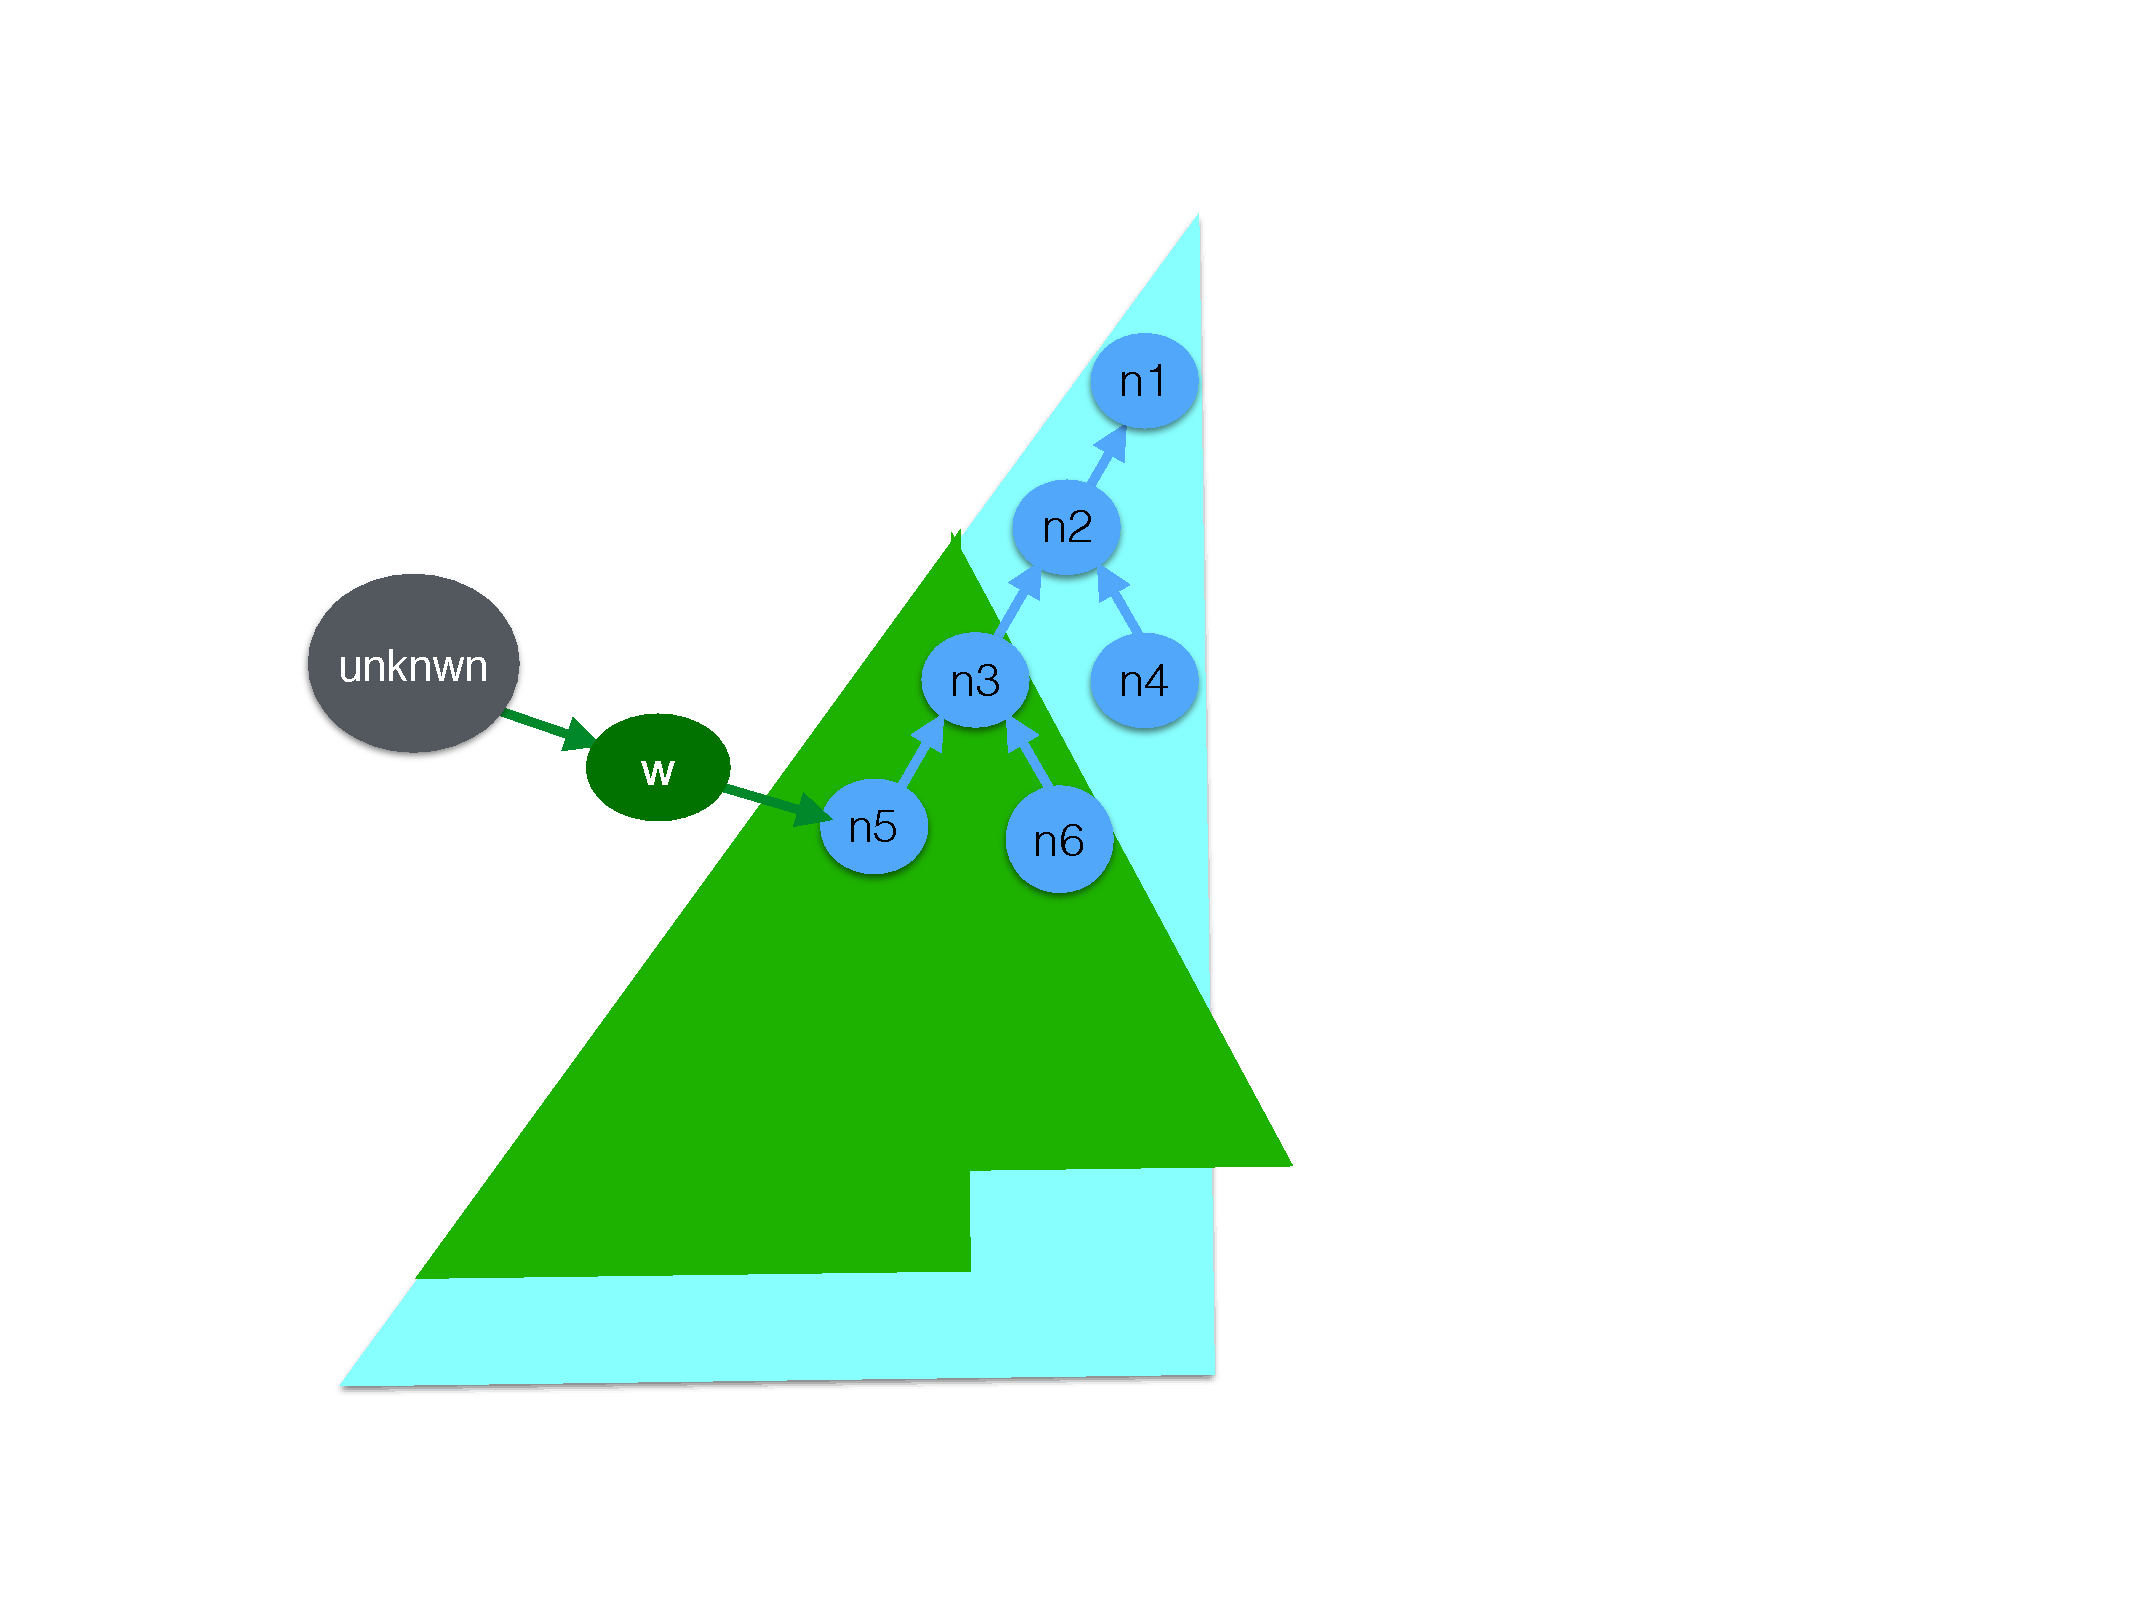
\includegraphics[width=\linewidth, trim=145  320 60 105,clip]{diagrams/DOM.pdf}
% x y z w
% y seems to eat up the bollom
% y=320 is good
% x eats space from left, if you increase it the diagram decreases from left
% w eats space from top, if you increase it the diagram decreases from top
% w=100 is good
%\includegraphics[page=3, width=\linewidth, trim=150  270 40 150, clip]{diagrams/snmalloc.pdf}\sdcomment{I think we need to change the diagram so that it says small slab.}
\strut \\
\strut \\

\end{minipage}
\end{tabular}
 \vspace*{-4.5mm}
\caption{\prg{Wrapper}s protecting \prg{Node}s }
\label{fig:WrapperUse}
\end{figure}

Even though we know nothing about the \prg{unknown} object or
its \prg{untrusted} function, and even though the call gives
to \prg{unknown} access to \prg{w}, which in turn has transitively
access to all \prg{Node}-s in the tree, we know that %the call to
the \prg{untrusted} function is guaranteed not to line 10 will not
affect the \prg{property} fields of the nodes \prg{n1}, \prg{n2},
and \prg{n4}.  Thus, the assertion on line 12 is guaranteed to
succeed.  The question is how do we specify \prg{Wrapper}, so as to be
able to make such an argument. %prove this assertion.

A specification of the class \prg{Wrapper} in the traditional
style, \eg \cite{Leavens-etal07} (\cf appendix \ref{DOM:traditional})
consists of pairs of pre- and post- conditions for each of the
functions of that class. Each such pair gives a {\em sufficient}
condition for some effect to take place: for example the
call \prg{w.setProperty(i,prp)} where \prg{i} is smaller
than \prg{w.height} is a sufficient condition to modify \prg{property}
of the \prg{i}-th parent of \prg{w.node}. But we do not know what
other ways there may be to modify a node's \prg{property}.  A broken
wrapper could accidently permit access to nodes one or two levels
about the expected height due to off-by one errors. More seriously,
a malicious wrapper could offer a
back-door public accessor method that leaks the underlying DOM
object through the wrapper, return direct access to any of the
other nodes in the DOM, or even to queue a task to
delete every property at midnight GMT on 29 March 2019. All of these errors are possible while
preserving the pre- and post- conditions expected of a \prg{Wrapper}. 
What is needed here is some way to specify the \emph{necessary
conditions}
under which some change could be made: if some external client is to
change a node's property, then  that client must have either direct
access to a node in that DOM tree, or indirect access via a wrapper
configured so that it can change the affected node.
Thus,
 \sdcomment{Shall we say the following, or does it break the flow?  
"Moreover, on line 10 we do not know which functions are called
on \prg{w}."
\kjx{I put that in and expanded on it. We need to explain the issues I think}
I do not see where it is}

% I think the below should be clear by niw
% In this work, we propose \emph{holistic specifications}, which
%describe the behaviour of an abstract data type as a whole, taking all
%possible method calls into account. Such holistic specifications
%emphasize the \emph{necessary conditions} for some effect to take
%place over the sufficient conditions as in traditional
%specifications. In our example:

\begin{quote}
The \emph{necessary} condition for the modification of \prg{nd.property} for some \prg{nd} of class \prg{Node}  is either access to some   \prg{Node} in the same tree, or  access to a \prg{w} of class \prg{Wrapper} where the \prg{w.height}-th parent of \prg{w} is an ancestor of \prg{nd}.
\end{quote}


With such a specification we can prove that the assertion on line 12
will succeed. Crucially, we can ensure that all future updates of
the \prg{Wrapper} class must continue to meet that specification,
guaranteeing the protection
of the \prg{Node} data. 
%
% Having justified the need for  necessary conditions in specifications, 
%
To give a flavour of \Chainmail, we use it  express the requirement from above:
%  This  gives us the opportunity to  demonstrate primitives for time ($\Future{\_}$) and authority ($\Changes{\_}$ and $\Using {\_} {\_}$).
 % and   more traditional relations between objects ( $\prg{nd}.\prg{parnt}^k\!=\! ...$):
% $\strut$ 
\vspace{.1cm}

\noindent
% \begin{quote}
$\forall \prg{S}:\prg{Set}.\forall \prg{nd}:\prg{Node}.$\\
$[\ \ {\Using{\Future {\Changes {\prg{nd.property}}}}  {\prg{S}}}$ \\
$\strut  \ \ \longrightarrow$\\
$\strut \ \ \ \exists \prg{o}:\prg{Object}[\ \prg{o}\in\prg{S}\ \ \wedge\ \ \neg(\prg{o}:\prg{Node})\ \ \wedge\  \ \neg(\prg{o}:\prg{Wrapper})\ \ \ \wedge \  $\\
$ \strut\ \ \  \ \ \ \ \ \ \ \ [\ \exists \prg{nd}':\prg{Node}. \CanAccess{\prg{o}}{\prg{nd}'}\  \ \ \  \vee$\\
$ \strut\ \  \ \  \ \  \ \ \ \ \ \ \ \exists \prg{w}:\prg{Wrapper}.\exists k\!:\!\mathbb{N}.
% $\\ $ \strut \ \ \ \ \ \ \ \ \ \ \ \ \ \ \ \ \  \ \ \
  (\ \CanAccess{\prg{o}}{\prg{w}}  \ \wedge\ \prg{nd}.\prg{parnt}^k\!=\!\prg{w.node}.\prg{parnt}^{\prg{w.height}}) \ \ \ ]\ ]$\\
$ ]$
% \end{quote}

\vspace{.1cm}

% \noindent
That is, if the value of \prg{nd.property} is modified
($\Changes{\_}$) at some future point ($\Future{\_}$) and if reaching
that future point involves no more objects than those from set \prg{S}
(\ie ${\Using{\_} {\prg{S}}}$), then at least one (\prg{o}) of the
objects in \prg{S} is not a \prg{Node} nor a \prg{Wrapper},
and \prg{o} has direct access to some node
($\CanAccess{\prg{o}}{\prg{nd}'}$), or to some wrapper \prg{w} and
the \prg{w.height}-th parent of \prg{w} is an ancestor of \prg{nd}
(that is,
$\prg{parnt}^k\!=\!\prg{w.node}.\prg{parnt}^{\prg{w.height}}$).
% It is important to clarify what we mean by ``access''. 
Definitions of these concepts appear later
(Definition \ref{def:valid:assertion}), but note that our ``access''
is intransitive: $\CanAccess x y$ holds if either \prg{x} has a field
pointing to \prg{y}, or \prg{x} is the receiver and \prg{y} is one of
the arguments in the executing method call.
 
In the next sections we proceed with a formal model of our model. In the appendix we discuss more -- and simpler -- examples.
We chose the DOM for the introduction, in order to give a flavour of the \Chainmail features.
 


\section{DOM Wrappers -- code and traditional Specification}
\label{DOM:traditional}

\kjx{this stuff should go with the DOM example,
  either in motivation, or as second example after formalism?}

\kjx{merge in when we first talk about language:}
We write our code in a small, fictitious, class-based, dynamically
typed, imperative programming language. All functions are public, \ie
may be called by any other object, and all fields are private, \ie may
be read or written only by the object itself. 

\begin{figure}[htb]
\begin{tabular}{llll}
&
\begin{minipage}{0.45\textwidth}
\begin{lstlisting}
class Node(par,prop){

  fld parnt = par;
  fld property = prop;
  fld children = new array[10];
  fld maxChild=0;
  children[maxChild++]=this
  
  func getParent(){
       parnt 
  }  
  func getChild(i){
       children[i] 
  }
  func setProperty(prp){
       property = prp 
  }  
  func setChild(nd){
       children[i] = nd
  }  
}
\end{lstlisting}
\end{minipage}
& & 
\begin{minipage}{0.40\textwidth}
\begin{lstlisting}
class Wrapper(nd,hgt){

  fld node=nd;
  fld height=hgt;

  func setPropety(i,prp){
    if (i>height){ 
       return 
    } 
    else  
    {  nd=node;  
       while (i>0){
          nd=nd.getParent();
          i--;    };
        nd.setProperty(prp); }
  }    
  func getChild(i){ 
    Wrapper(node.getChild(i),
                    height+1); 
 }                           
}
\end{lstlisting}
\end{minipage}
\end{tabular}
 \vspace*{-7mm}
\caption{\prg{Node}  and \prg{Wrapper} }
\label{fig:DOM}
\end{figure}

The figure needs some beautification

\begin{figure}[htb]
\begin{lstlisting}
class Wrapper(nd,hgt){

  fld node=nd;
  fld height=hgt;

  func setPropety(i,prp)
  // PRE:  true
  // POST:
  //     (  i not a number or i>this.height ) --> modifies nothing  
  //     &&
  //     i<=this.height -->  (  modifies = { this.node.parnt^i.property }
  //                          &&
  //                          this.node,parnt^i.property == prp )
  {
    if (i>height){     return     } 
    else  
    {  nd=node;  
       while (i>0){   nd=nd.getParent();  i--;    };
        nd.setProperty(prp); }
  }    
  func getChild(i)
  // PRE:  true
  // POST:  modifies: nothing
  // RETURNS: i-th child of this
  
  {    Wrapper(node.getChild(i),   height+1);   }                           
}
\end{lstlisting}
 \vspace*{-7mm}
\caption{\prg{Wrapper} specification}
\label{fig:WrapperSpec}
\end{figure}

In Figure \ref{fig:WrapperSpec} we  outline a specification of the class \prg{Wrapper} in the ``traditional style''. Each function has a pore and a post conditon. Because the functions may be called by any, unchecked code, the preconditions are not stronger than \prg{true}. The functions need to behave correctly under all possible circumstances.  The post-condition of \prg{setPropery} guarnatees that if the argument is not a number or if it is larger than the \prg{height} of the wrapper, then nothing is modified. If on the other hand, the argument is smaller or equal to the \prg{height}, then the \prg{property} of the \prg{i}-th parent will be set to \prg{prp}, and nothing else will be modified.





\section{Example -- DAO}
The DAO  {(Decentralised Autonomous Organisation)}~\cite{Dao}  is a famous Ethereum contract  which aims to support
collective management of funds,  and to place power directly in the
hands of the owners of the DAO
rather than delegate it to directors.
Unfortunately, the DAO was not robust:
a re-entrancy bug   exploited in June 2016 led  to a loss of   \$50M, and
a hard-fork in the  chain ~\cite{DaoBug}.
%
%In a similar style as that  of the ERC20 spec earlier,
%We can give a \Chainmail~specification
With holistic specifications  we can  write a succinct requirement that a
DAO contract should always be able to repay any owner's money.
Any contract which satisfies such a holistic specification cannot demonstrate the DAO bug.
 
Our specification consists of \jm[]{two} requirements.
First, that the DAO always holds at least as 
much money as any owner's balance\jm[I added this to make it clear that we don't need to talk about all owners]{, and thus is always able to repay any owner}.
%  \james{ALL owners? or does that follow?} 
To express this we use 
the field \prg{balances} which is a mapping from participant's addresses to 
numbers. Such mapping-valued fields exist in Solidity, but 
\jm{in \Chainmail it could be a real field or a ghost field.}
%they could
%also be taken to be ghost fields~\cite{ghost}.
  
\vspace{.1cm}

\noindent
 \strut \hspace{0.5cm} $\forall \prg{d}:\prg{DAO}.\forall \prg{p}:\prg{Any}.\forall\prg{m}:\prg{Nat}.$\\
\strut \hspace{0.5cm} $[\ \ \prg{d.balances(p)}=\prg{m}  \ \ \  \longrightarrow  \ \ \ \prg{d}.\prg{ether}\geq \prg{m} \ \ ] $
  \jm[should spec 2 be done in classical spec? extend chainmail?]{}

 

%\kjx{combined defn ensuring enough eth at the time repayment is made:\\
%\noindent
% \strut \hspace{0.5cm} $\forall \prg{d}:\prg{DAO}.\forall \prg{p}:\prg{Any}.\forall\prg{m}:\prg{Nat}.$\\
%\strut \hspace{0.5cm} $[\ \ \prg{d.balance(p)}=\prg{m}
% \ \wedge \ \Calls{\prg{p}}{\prg{repay}}{\prg{d}}{\_}  $\\
% $\strut \hspace{5.5cm}   \ \ \  \longrightarrow  \ \ \  \Future{\Calls{\prg{d}}{\prg{send}}{\prg{p}}{\prg{m}}
% \wedge \prg{d}.\prg{ether}\geq \prg{m}}\ \ ] $
%\vspace{.1cm}
%}
%
%\kjx{negative example for talk, upping funds not calling send:\\
%\noindent
% \strut \hspace{0.5cm} $\forall \prg{d}:\prg{DAO}.\forall \prg{p}:\prg{Any}.\forall\prg{m}:\prg{Nat}.$\\
%\strut \hspace{0.5cm} $\ \ \Calls{\prg{d}}{\prg{send}}{\prg{p}}{\prg{m}}
% \strut \ \ \  \longrightarrow  \ \ \  \prg{d}.\prg{ether}\geq \prg{m}$\\
% % SD thinks the last  \longrightarrow sgould be wedge
%  $\strut \ \ \  \longrightarrow  \ \ \  \prg{p.funds}
%  = \Prev{\prg{p.funds}} + \prg{m}$
%\vspace{.1cm}
%}


\noindent
\sd{\jm{Second}, that the balance of an owner is a function of its balance in the previous step,
or the result of it joining the DAO, or asking to be repaid \etc.}
 
\noindent
$\strut \hspace{0.5cm} \forall \prg{d}:\prg{DAO}.\forall \prg{p}.\forall:\prg{m}:\prg{Nat}.$\\
$\strut \hspace{0.5cm} [ \ \ \  \prg{d.Balance(p)}=\prg{m} \ \ \  \longrightarrow   
 \ \  \ \ 
  [ \  \ \Prev{\Calls{\prg{p}}{\prg{repay}}{\prg{d}}{\_}}\, \wedge\, \prg{m}=\prg{0} \ \ \ \ \vee $\\
$\strut \hspace{5.7cm}      
\Prev{\Calls{\prg{p}}{\prg{join}}{\prg{d}}{\prg{m}}}  \ \ \ \ \vee   $\\
 $\strut \hspace{5.7cm}  ... \  ]$ \\
%                         
%                         $ \left\{
%                            \begin{array}{ll}
%                             \prg{0}, & \hbox{if}\ Prev(Call(\prg{p},\prg{d.repay(),\_})    \\
%                             \vee
%                             \\
%                             \prg{m},  & \hbox{if}\  Prev(Call(\prg{p},\prg{d.join(),m}))   \\
%                             ..., & ...
%                           \end{array}
%                         \right.    $\\
$\strut \hspace{0.5cm} ] $


\jm[reworded]{In order to reflect the financing and repayments of proposals, more cases are needed, however they can be expressed with the concepts described so far.}
 

\jm[added break before paragraph]{}
The requirement that \prg{d} holds at least \prg{m} ether precludes the DAO bug,
in the sense that  any contract satisfying that spec cannot exhibit  the  bug:   a contract
which satisfies the spec  is guaranteed to always have enough money to satisfy all \prg{repay} requests.
This guarantee  holds, regardless of how many functions there are in the DAO.
In contrast, to preclude the DAO  bug with a classical spec, one would need to write a spec for each of the
DAO functions (currently 19), a spec for each function of the auxiliary contracts used by the DAO,
and then study their emergent  behaviour.

These 19 DAO functions   have several different concerns:
who may vote   for a proposal, who is eligible to submit a proposal,
how long the consultation period is for deliberating a proposal, what
is the quorum, how to chose curators, what is the value of a token,
Of these groups of functions, only  a handful affect the balance of a
participant. Holistic specifications allow us to concentrate on aspect of DAO's behaviour across \emph{all} its functions.

\jm[]{
\noindent
It is notable that Chainmail is only able to specify how client code interacts
with the DAO, and not how the DAO interacts with client code.
A third specification might say that when an owner asks to be repaid, she is sent all her money.\\
\vspace{.1cm}
\noindent
 \strut \hspace{0.5cm} $\forall \prg{d}:\prg{DAO}.\forall \prg{p}:\prg{Any}.\forall\prg{m}:\prg{Nat}.$\\
\strut \hspace{0.5cm} $[\ \ \prg{d.balance(p)}=\prg{m}
 \ \wedge \ \Calls{\prg{p}}{\prg{repay}}{\prg{d}}{\_}  $\\
 $\strut \hspace{5.5cm}   \ \ \  \longrightarrow  \ \ \  \Future{\Calls{\prg{d}}{\prg{send}}{\prg{p}}{\prg{m}}}\ \ ] $  
\vspace{.1cm}\\
The above specification is not legal Chainmail, as \Calls{\prg{d}}{\prg{send}}{\prg{p}}{\prg{m}}
specifies a method call made by internal DAO code. 
This example specification indicates that Chainmail might benefit from
the ability to specify calls to external code.
}


\section{Example -- Purse and Mint}
take from our earlier works

In two versions: one where there is a ledger inside the Mint, and one where the Mint has no path to the Purses. This will serve to demonstrate how \prg{internal} is supposed to work.

\section{Example -- Membrane}

TODO - take from ShuPeng's thesis
}

\begin{definition}[Time, Permission, Authority,  and Space ]
\label{def:permission}
Given a module $\M$, identifiers \code{x} and \code{y}, expression $\sE$, and runtime configuration $\sigma$, and a set of addresses $S$,
we define validity of the assertions   .... as follows:

\begin{itemize}
\item
$\M,\sigma \models  \Future \A$\ \ iff\ \  $\exists \sigma'.\, [\ \ \M,\sigma \leadsto^* \sigma' \ \wedge \ \M,\sigma' [\overline{x \mapsto \sigma(x)}]\models \A, \mbox{ where } \overline{x}=Free(\A)\   ]$.
\item
$\M,\sigma \models  \Past \A$\ \   iff\ \  $\exists \sigma_1,....\sigma_n, k\!\in\![1..n-1).\ [ \Initial {\sigma_1}\  \wedge\ \sigma_n=\sigma\ \wedge\ \forall i\!\in\![1..n).\ \M,\sigma_i\leadsto  \sigma_{i+1}  $\\
\strut \hspace{5.7cm} $\ \wedge \  \ \M,\sigma_k[\overline{x \mapsto \sigma(x)}]\models \A, \mbox{ where } \overline{x}=Free(\A)\  ]$.


\item
 $\sigma\!\mid_S$ denotes a {\em restriction} of $\sigma$ to the objects from the set $S$. That is, the domain of
 the heap in $\sigma\mid_S$ is $S$, and otherwise,  $\sigma\mid_S$ is identical to $\sigma$. An example appears in figure \ref{fig:DiagramRestricted}.
 \item
$\M,\sigma  \models \Using{\A}{\prg{S}}$  \  \ iff \ \
  $ \M,\sigma\!\mid_S\, \models \A $, where   $S=\interp {\prg{S}} {\M,\sigma} $.
 \item
 $\M,\sigma  \models \Calls {m}$ \ \ iff \ \ the method call in the current frame in $\sigma$ is
 \prg{m}\footnote{We will express this precisely  when we have the full definition of $\sigma$}
\end{itemize}
\end{definition}

\begin{figure}[btph]
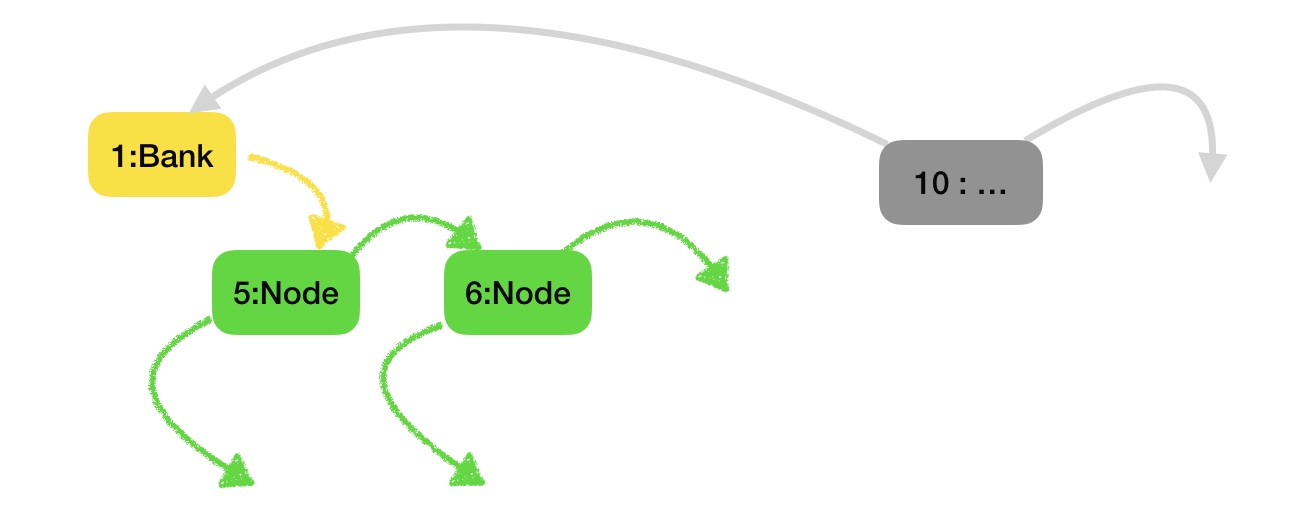
\includegraphics[width=10cm,height=4cm]{diagram2}
 \caption{Configuration from Fig. \ref{fig:Diagram} restricted to witness \{ \prg{1}, \prg{5}, \prg{6}, \prg{10} \}}
  \label{fig:DiagramRestricted}
  \end{figure}

Note that $\CanAccess{\prg{x}}{\prg{y}}$ is reflexive but  not transitive and not symmetric.

Also note the difference between $\Using{(\Future{\A})}{\prg{S}}$ and $\Future{(\Using{\A} }{\prg{S}})$.
For example,  the assertion  $\Using{(\Future{\prg{x}.\prg{f}=\prg{z}})}{\prg{S}}$ expresses that the current execution
leads to a future configuration  where
$\prg{x}.\prg{f}=\prg{z}$ will hold, and that the set \prg{S} suffices to witness this execution, while the assertion
$\Future{(\Using{{\prg{x}.\prg{f}=\prg{z}} }}{\prg{S}})$  expresses that the current execution
leads to a future configuration   where
$\prg{x}.\prg{f}=\prg{z}$ will hold and where  the set \prg{S} suffices to witness
that fact.
For example, take a configuration $\sigma$ where variable \prg{x} maps to some object \prg{31}, and where \prg{31} has a field \prg{f}
pointing to \prg{32}, and \prg{32} has a field \prg{f}
pointing to \prg{33}, and variable \prg{z} maps to  \prg{33}. Assume also that the expression to be executed in $\sigma$ starts with
\prg{x.f}=\prg{x.f.f}. Then we have that
$\M,\sigma  \models \Future{(\Using{{\prg{x}.\prg{f}=\prg{z}} }{\{\prg{x},\prg{z}\}})}$,
but
$\M,\sigma  \not\models \Using{(\Future{\prg{x}.\prg{f}=\prg{z}})}{\{\prg{x},\prg{z}\}}$.
On the other hand
$\M,\sigma  \not\models \Using{(\Future{\prg{x}.\prg{f}=\prg{z}})}{\{\prg{x},\prg{x}.\prg{f},\prg{z}\}}$

In general, for all $\M$ and $\sigma$, we have that
 $\M,\sigma \models  \Using{(\Future{\A})}{\prg{S}}$ implies $\M,\sigma \models \Future{(\Using{\A} }{\prg{S}})$, and that
 $\M,\sigma \models \Future{(\Using{\A} }{\prg{S}})$ implies that there exists a set $\prg{S}'$ such that
 $\M,\sigma \models  \Using{(\Future{\A})}{(\prg{S}\cup\prg{S'})}$.

\vspace{.2in}
We will prove that

\begin{lemma}[Preservation of validity and module linking]

$\M,\sigma \models \A$  \ \ \ then\ \ \ \   for all $\M'$ with $\M\link\M'$ is defined:\ $\M\link\M',\sigma \models \A$.
\end{lemma}




\subsection{Invariants}

We define below the meaning of invariants.\footnote{This part is as we had defined previously, with two simplifications: a) we do not need to worry about the $\obeys$-predicate here, and b) we do not distinguish the names of the classes and the names of participants in interfaces.}
The assertion $\M   \models\  \A$ requires that  the assertion $A$ is satisfied
in all reachable states.

\begin{definition}[Invariants]
\label{def:invariant}
\noindent
For a module $\M$  and assertion $\A$ we define:\\

 \begin{itemize}
 \item
$\M   \models\  \A$\ \ \  iff\ \ \ \
% $\strut\SP\SP$
$\forall \M'.\, \forall \sigma\!\in\!\Arising(\M'*\M).\ \M'*\M,\sigma \models \  \A$
 \end{itemize}
\end{definition}

The use of the set of configurations from $\Arising(\M'*\M)$ reflects that policies
 need to hold in an {\em open} world, where
we link against {\em any} module $\M'$,
about which we know nothing.

\subsection{Implication and equivalence}

\begin{definition}
\label{def:impl:equiv}
\noindent
For a module $\M$  and assertions $\A$  and $\A'$, we define strong equivalence and implication ($\equiv$ and $\sqsubseteq$), as well
as   weak equivalence and implication ($\approxeq$ and $\weakImplies$)  as follows:


 \begin{itemize}
\item
$\M   \models\  \A \strongImplies \A'$  \ \ \ \ iff \ \ \ \
$\forall \M'.\, \forall \sigma\!\in\!\Arising(\M'*\M).[\ \ \  \M'*\M, \sigma \models \A \  \ \  \longrightarrow\  \ \  \M'*\M, \sigma \models \A'\ \ \ ]$
 \item
$\M   \models\  \A \equiv \A'$ \ \ \ \ iff \ \ \ \
$\M   \models\  \A \strongImplies \A'\ \  \wedge \ \  \M   \models\  \A' \strongImplies \A$
%$\forall \M'.\, \forall \sigma\!\in\!\Arising(\M'*\M):\ \ \  \M'*\M, \sigma \models \A \  \ \longleftrightarrow\   \ \M'*\M, \sigma \models \A'$
\item
$\M   \models\   \A \weakImplies \A'$  \ \ \ \ iff \\ \ \ \ \ \ \
\strut  \hspace{1cm}  $\forall \M'.\, \forall \sigma\!\in\!\Arising(\M'*\M).\,\M'*\M, \sigma \models \A$ \  \ \  $\longrightarrow$\  \ \
$\forall \M'.\, \forall \sigma\!\in\!\Arising(\M'*\M).\,\M'*\M, \sigma \models \A'$
\item
$\M   \models\  \A \approxeq \A'$   \ \ \ \ iff \ \ \ \ \
$ \M  \models  \A \weakImplies \A' \   \ \wedge\   \  \M  \models  \A' \weakImplies \A$
 \end{itemize}
\end{definition}

The definitions from above are applicable to the empty module, eg  $\models\  \A \equiv \A'$ iff   all modules $\M$ satisfy $\M \models\  \A \equiv \A'$.
The following properties hold:

\begin{lemma}
For all modules \M, assertions \A and \A':

 \begin{itemize}
 \item
$\M   \models\  \A \equiv \A'$  \ \ \ implies \ \ \  $\M   \models\  \A \simeq \A'$
\item
$\M   \models\  \A \strongImplies \A'$  \ \ \ \ implies  \ \ \ \
$\M \models \A \weakImplies \A$
\item
$\M \models   \Using{(\Future{\A})}{\prg{S}}\ \strongImplies\ \Future{(\Using{\A} }{\prg{S}})$
\item
$ \M \models\  \Future{\A}\rightarrow \A' \  \  \weakImplies \ \ \A\rightarrow\Past{\A'}$
\item

 \end{itemize}
\end{lemma}

\paragraph{Space-Monotonicity}\footnote{Not sure how useful this concept is}

\begin{definition}[Space-Monotonicity]
We call an assertion $\A$ {\em space-monotonic} in $\M$, iff for all set expressions $\prg{S}$ and  $\prg{S}'$,
  % $\M,\sigma\models ( \prg{S} \subseteq \prg{S}'\ \wedge\  \Using{\A, \prg{S}}) \ \strongImplies\  (\Using{\A, \prg{S'}})$
%\end{definition}\footnote{If we unfold the definitions, we obtain that
% $\A$ is space-monotonic in $\M$, iff for all set expressions $\prg{S}$ and  $\prg{S}'$
 and all $\sigma\in\Arising({\M})$:
 \\
  If  $\M,\sigma\models  \prg{S} \subseteq \prg{S}'$ and $\M,\sigma\models  \Using{\A} {\prg{S}}$, then
$\M,\sigma\models  \Using{\A}{ \prg{S'}}$
\end{definition}

We prove space monotonicity for some assertions

\begin{lemma}[Space-Monotonicity for change and access]
$ ~ $

\begin{itemize}
\item
${\Changes \sE} $ is space-monotonic.
\item
$\CanAccess {\prg{x}}{\prg{y}}$ is space-monotonic.

\end{itemize}
\end{lemma}

Not all assertions  are not space-monotonic. E.g. $\forall a:\prg{Account}.\prg{a.balance}\geq 3$ is not space-monotonic.


The following lemma would be nice to have -- otherwise we will need to change the definition of monotonicity.

\begin{lemma}[Space-Monotonicity and module linking]
If $\A$ is space-monotonic with $\M$, then it is also space-monotonic with $\M*\M'$.
\end{lemma}


 \section{Specifications for Robustness Policies}

 We now use the concepts introduced in the earlier sections to specify various robustness policies

 \subsection{Specification of \Pol 2  and   \Pol 4}

We    give a formal definition of \Pol 2 and  \Pol 4, using the concepts defined earlier in  Definition \ref{def:permission}: %

\begin{definition}
\label{def:pol2}
We define  what it means for an object \prg{o} to be internal to a bank's data structure, an then define \Pol 2  and   \Pol 4  as follows:

%  \noindent
$\prg{Internal}(\prg{b})$ \ \  $\triangleq$ \ \
$\{\ \prg{o}\ \mid\  \prg{b}:\prg{Bank}\ \ \wedge \ \ (\ \prg{o} = \prg{b}\ \ \vee\  \ \prg{o}:\prg{Account}\wedge \prg{o}.\prg{myBank}=\prg{b}$\\
\strut \hspace{7.3cm} $\ \ \vee\ \ \ \exists k. \ \prg{b}.\prg{ledger}.\prg{next}^k = \prg{b})\ \ \ \ \}$


$\prg{Internal}'(\prg{a})$ \ \  $\triangleq$ \ \
$\{\ \prg{o}\ \mid\  \prg{a}:\prg{Account}\ \ \wedge \ \
 \prg{a}.\prg{myBank} :\prg{Bank}\ \wedge\  \prg{o}\in \prg{Internal}(\prg{b})\ \}$


 \vspace{.2cm}

  \Pol 2\ \  $\triangleq$ \ \
  $\forall \prg{b}.\forall \prg{S}.
  [ \ \  \prg{b}:
  \prg{Bank}\ \wedge\ \prg{this}\neq\prg{b}\ \wedge\ \ \Using{(\Future\Changes{\prg{b.currency}})}{\prg{S}} \ \ \ \ \longrightarrow \ \  $\\
   \strut $~ $ \ \ \ \hspace{1.7in}  \hfill
 $\exists \prg{o}. \ [ \ \
  \prg{o}\in \prg{S}\   \wedge\  \CanAccess{\prg{o}}{\prg{b}}\ \wedge\     \prg{o}\notin\prg{Internal}(\prg{b})  \ \ ]\ \ ]$


 \vspace{.1cm}
% \noindent
    \Pol 4\ \  $\triangleq$\ \ $\forall \prg{a}.\forall \prg{S}.\ [ \ \  \prg{a}:\prg{Account}\   \wedge\   \prg{this}\neq\prg{a} \ \wedge\ \Using{(\Future\Changes{\prg{a.balance}})}{\prg{S}}\ \ \   \
    \longrightarrow$ \\
 $\strut \hspace{3.9cm} \hfill \exists \prg{o}.\ [\, \prg{o}\in \prg{S}\ \wedge \ \CanAccess{\prg{o}}{\prg{a}}\ \wedge  \ \prg{o} \notin\prg{Internal}'(\prg{a}) \ ] \ \ \ \ ]$

\end{definition}

\paragraph{Discussion}
In other words, \Pol 2  mandates that the elements of the data structure (ie the elements from $\prg{Internal}(\prg{b})$) cannot be used (are not sufficient) to  change the currency of the bank. If a computation takes place inside the set \prg{S}, and {\em in the current state} in \prg{S}
all accesses to the bank go through elements of the data structure (ie the \prg{Account} objects),\footnote{Say why we can ignore \prg{Node} objects} then we have a guarantee that the computation will not affect the currency.
For example, if a computation takes place in the context of objects \prg{1}, \prg{2}, \prg{3}, \prg{4}, \prg{5}, \prg{7}, \prg{20} and \prg{21}, and the current receiver is no \prg{1}, then we have a guarantee that the currency of \prg{1} will not be affected. So, even through \prg{1} is involved in the computation, because there is no {\em external} access to it, we have a guaratee that the method \prg{makeAccount} will not be called on it.

An alternative way of expressing \Pol 2 is as follows:


 \Pol 2\ \  $\equiv$ \ \
  $\forall \prg{b}.\forall \prg{S}.
  [ \ \  \prg{b}:
  \prg{Bank}\ \wedge\   \prg{b}\neq\prg{this}\ \wedge\  \forall \prg{o} \in \prg{S}.\, [\ \prg{o}\in\prg{Internal}(\prg{b}) \ \vee\  \neg  \CanAccess{\prg{o}}{\prg{a}}  \ \ ]$
\\ \hfill \strut $~   \ \ \ \hspace{1.7in}  \  \ \longrightarrow \ \ \ \neg(
 \Using{(\Future\Changes{\prg{b.currency}})}{\prg{S}})\   \  \ \ ]$

\vspace{.01in}
% TO\_DO: discuss the difference between  $\Using{(\Future\Changes{\prg{b.currency}})}{\prg{S}})$, and
% $\Future{(\Using{\Changes{\prg{b.currency}}{\prg{S}})}}$.

\vspace{.01in}
\Pol 2  guarantees
that if an object \prg{o}$\neq$\prg{b} may affect the value of \prg{b.Currency} only if the  objects
involved in the process of affecting the value of \prg{b.Currency}  include at least an object $\prg{o}'$
which had direct access to \prg{b}, and
whose class is  not  \prg{Account}. Stated positively, this policy mandates
that exporting an \prg{Account} to an environment will not affect the \prg{Currency} of \prg{b}.
In other words,
\prg{Account}s protect the integrity of the \prg{Bank}'s currency.


In more detail, by applying  Definition \ref{def:invariant} on Definition \ref{def:pol2}, the  meaning of policy \Pol 2
  is, that a runtime configuration $\sigma$ satisfies  \Pol 2  if whenever the current receiver in $\sigma$
 is not a \prg{Bank} object, and the execution of $\sigma$ leads to another runtime configuration $\sigma'$
 with a different value for \prg{b.Currency}, then the objects involved in the execution from
 $\sigma$ to $\sigma'$ include at least one object which had direct access to \prg{b}.
 Note that this direct access needs to exist at the beginning of   the execution, \ie at $\sigma$.
 Formally:

 \noindent
 $\M, \sigma \models  \Pol 2$\\$ \strut \ \ \ \  \ \  \longleftrightarrow $\\
 $\forall \prg{b}.\forall S.\ [ \ \ \ \ \M, \sigma \models \prg{b}:\prg{Bank}\ \wedge\
 \sigma(\prg{b})\neq \ \sigma(\prg{this}) $\\
 $\strut \hspace{2.1cm}  \wedge \
 \ \exists\sigma'.(\ \ \ \ \M, \sigma\mid_S \leadsto^* \sigma'\
\ \wedge\ \interp {\prg{b.Currency}}{\M,\sigma}\neq \interp {\prg{b.Currency}}{\M,\sigma'[\prg{b}\mapsto\sigma(\prg{b})]}\ )$\\
$\strut \hspace{4.7cm} \longrightarrow$ \\
 $\strut \hspace{2.7cm}  %\exists \prg{o}. (\ \  \sigma(\prg{o}) \!\!\in\!\!\prg{S}\ \
 \exists \prg{o}. (\ \ \prg{o} \!\in\!S\ \
  \wedge \ \ \M, \sigma \models \CanAccess{\prg{o}}{\prg{b} }\ \wedge \  \prg{o}\notin \prg{Internal}(\prg{b}) \   \ ) \ \ \ \ \ \ \  ]$



\subsection{Specifying  "no leaks"}

This is a family of guarantees that Dean seemed especially interested in, when we discussed in March in London.
For the particular example, we want to express that

\begin{description}
\item[\Pol 7]
The \prg{Bank} does not leak out of the \prg{Bank}/\prg{Account} system
%\item[Pol\_7]
%The \prg{Accounts} do  not leak out of the \prg{Bank}/\prg{Account} system
\end{description}

And we give a formal specification

\begin{definition}[Banks do not leak]
\label{def:bankNoLEak} We define \Pol 7 as follows:

\Pol{7}\ \  $\triangleq$\ \ $\forall \prg{b}.\forall \prg{S}.\ [  \ \ \prg{b}:\prg{Bank}\ \wedge\  \prg{o}:\prg{Object}\  \wedge\   \neg(\CanAccess{\prg{o}}{ \prg{b}})\ \wedge\   \Using {(\Future{\CanAccess {\prg{o}}{\prg{b}}})} {\prg{S}} $
 \\  $\strut$ \hspace{4cm}
  $\longrightarrow$
 $\strut \hspace{0.5cm}  \exists \prg{o}'.\ [\, \prg{o}'\in \prg{S}\ \wedge \  \CanAccess{\prg{o}'}{ \prg{b} }\ \wedge\   \prg{o}' \notin \prg{Internal}(\prg{b}) \, ) \ ] \  \  \ \  ]$

%\hspace{.1cm}
%{\bf {Pol\_8}}\ \  $\equiv$\ \ $\forall \prg{o},\prg{b}, \prg{o}'\forall \prg{S}.\ [  \ \ \prg{b}:\prg{Bank}\ \wedge \prg{o}\in\prg{Internal}({\prg{b}})\ \wedge\  \prg{o}':\prg{Object}\ \ \neg(\CanAccess{\prg{o}'}{ \prg{o}})\ \wedge\   \Using {(\Future{\CanAccess {\prg{o}'}{\prg{o}}})} {\prg{S}} $
% \\  $\strut$ \hspace{4cm}
%  $\longrightarrow$
% $\strut \hspace{0.5cm}  \exists \prg{o}''.\ [\, \prg{o}''\in \prg{S}\ \wedge \  \CanAccess{\prg{o}''}{ \prg{o} }\ \wedge\   \prg{o}'' \notin \prg{Internal}(\prg{b}) \, ) \ ] \  \  \ \  ]$
\end{definition}

In other words, \Pol 7 guarantees that objects that are internal to the bank \prg{b} do not leak access to it.
In more detail: if   objects  \prg{o} and \prg{b} exist  now, and \prg{o} does not have direct access to \prg{b} now, but obtains
access to \prg{b} through some computation which involves objects from the set \prg{S}, then at least one  object  from \prg{S} has
now direct access to   \prg{b} and this object is not internal to \prg{b}.

\section{Adherence to Policies}
\label{section:Adherence}
In this section we will outline the proofs that particular modules adhere to their specifications.
This serves to demonstrate the practicality of our approach.
In particular we will show two different versions fo the \prg{Bank}/\prg{Account} example (sections \ref{section:Adherence:ModuleOne} and \ref{section:Adherence:ModuleTwo}, and we will prove that
both satisfy the policies \Pol 2, \Pol 4, and \Pol 7, while they differ in the definition of \prg{Internal}.
But before doing that, in section \ref{section:GeneralPropertiesExecution}, we will study some further properties of execution.


\subsection{General properties of execution}\footnote{Find better title?}
\label{section:GeneralPropertiesExecution}

We will first define some further predicates which reflect over the program execution and prove
some general properties of program execution.

We call a locations set, \prg{L}, an expression which denotes a set of addresses and field identifiers, \eg, $\{\ (\prg{b},\prg{ledger}), (\prg{b}.\prg{ledger},\prg{balance})\ \}$ is such a locations set.

\begin{definition}[Framing]
Take arbitrary module \M, assertion \A, , ...

\begin{itemize}
\item
\interp{\prg{L}}{\sigma,\M*\M'} = ....
\item
$ \sigma\mid _L$ ....
\item
$\M, \sigma \models \prg{L} \frames \prg{e}$\ \ \ \  \ iff \ \ \ \ \
$\forall \M'.\forall \sigma'\!\in\!\Arising({\M*\M'}). \forall L.$\\
\strut \hspace{1cm} $  [ \ \ L=\interp{\prg{L}}{\M,\sigma}\, \wedge\,
 \sigma\mid _L= \sigma'\mid_L \ \   \longrightarrow\ \ \   \interp {\prg{e}}{\sigma,\M*\M'}  =  \interp {\prg{e}}{\sigma',\M*\M'}
\ \ ]$
\item
$\M  \models \prg{L} \frames \prg{e}$\ \ \ \  \ iff \ \ \ \ \
$\forall \M'.\forall \sigma\!\in\!\Arising({\M*\M'}). \ \M'*\M, \sigma \models \prg{L} \frames \prg{e}$
\item
$\M, \sigma \models \prg{L} \frames\A $\ \ \ \  \ iff \ \ \ \ \
$\forall \M'.\forall \sigma'\!\in\!\Arising({\M*\M'}). \forall L.$\\
\strut \hspace{1cm} $ [ \ \ L=\interp{\prg{L}}{\M,\sigma}\, \wedge\,
\sigma\mid _L= \sigma'\mid_L \ \   \longrightarrow\ \ \   [\ \M*\M',\sigma \models \A   \ \longleftrightarrow\ \M*\M',\sigma' \models \A
\ \ ] $
\item
$\M  \models \prg{L} \frames \A$\ \ \ \  \ iff \ \ \ \ \
$\forall \M'.\forall \sigma\!\in\!\Arising({\M*\M'}). \ \M'*\M, \sigma \models \prg{L} \frames \A$
\end{itemize}

\end{definition}

NOTE\_TO\_SELF: we need to think about whether we also need to make \prg{L} self-framing.
Also, rethink whether we need to stick new modules $\M'$ to the whole thing.
--
Also, the sets are not equal -- they are isomorphic. We can deal with isomorphisms, but
it has a high notation penalty. Can we pretend that they are equal? hmhhhhh


And then we can prove that changes in the interpretation or the validity require a change in the frame:

\begin{lemma}[Change in the context of framing]
Take arbitrary module \M, assertion \A, such that  $\sigma\in\Arising({\M*\M'})$

\begin{itemize}
\item
If  $\M  \models \prg{L} \frames \prg{e}$, and
$\M'*\M, \sigma \models \Using{(\Future{\Changes{\prg{e}}})}{\prg{S}}$, \\
then there exists a pair $(\prg{e}',\prg{f})$ , with
$\M,\sigma \models (\prg{e}',\prg{f})\in \prg{L}$\footnote{Sophia, you need to check this bit  what if \prg{z}
there is no handle in \prg{L}, eg what if \prg{L} talks about anonymous objects
\eg \prg{L} = $\{ o \ \mid o.\prg{myBank}=\prg{b} \}$?Here $o$ is anonymous. Also, do we need $\M$ or $\M'*\M$?}
and $\M'*\M, \sigma \models  \Using{\Future{\Changes{\prg{e}'.\prg{f}}}}{\prg{S}}$

\item
similar for
$\M'*\M, \sigma \models \Using{\Future{\Changes{\A}}}{\prg{S}}$
\end{itemize}

\end{lemma}

\begin{figure}[tbp]
\begin{lstlisting}
 class Bank {
   private field ledger;   // a Node

   Bank( )
     { ledger = null; }
   fun makeAccount(amt)
     { account = new Account(this);
       ledger = new Node(account, amt, ledger);
       return account; }
   fun deposit(source, destination, amnt)
     { sourceNd = ledger.getNode(source)
       destinationNd = ledger.getNode(destination)
       if (sourceNd!=null && destinationNd!=null && sourceNd.balance>amt) then
          { < sourceNd.balance = sourceNd.balance-amt
              destinationNd.balance = destinationNd.balance+amt > }
        else
          { return }               }
 }

 class Account {
   private field myBank;  // a Bank

   Account(aBank)
     { myBank = aBank;  }
   fun sprout( )
     // create Account in same Bank with 0 balance
     { return this.myBank.makeAccount(0)  }
   fun deposit(source, amnt)
     // if destination is an Account in myBank,  and  source holds enough money,
     // then transfer amnt from source into receiver
     { myBank.deposit(source,this,amnt) }
 }

  class Node{
   field balance;     // the  money held in theAccount a number
   field next;        // the next node
   field theAccount;  // the account

   fun getNode(account)
     { if (theAccount==account) then
           { return this }
       elseif (next!=null)
           { next.getNode(account) }
       else
           {  return null }            }	
 }
\end{lstlisting}
\caption{\MOne: First version of the Bank example, in detail}
\label{fig:BankDetailedOne}
 \end{figure}


We now think a bit more about changes in accessibility. The predicate  $\Gives(\prg{x},\prg{y},\prg{z})$ expresses
that \prg{x} passed to \prg{y} access to \prg{z}.

\begin{definition}[Giving]
For arbitrary module \M and $\sigma$, we define:

\begin{itemize}
\item
$\M,\sigma  \models \Gives(\prg{x},\prg{y},\prg{z})$\ \ iff \ \
$\sigma(\prg{this})$=$\sigma(\prg{x})$ \  $\wedge$ \
$\M, \sigma \models \neg (\MayAccess( \prg{y},\prg{z})\,)$ \ $\wedge$ \\
\strut \hspace{.9cm} $\exists \sigma'. \ [\  \M,\sigma \leadsto \sigma'  \  \wedge  \
 \M,\sigma' \models \MayAccess( \prg{y},\prg{z})\ ]$
\end{itemize}

\end{definition}

The following lemma says that any changes in accessibility witnessed\footnote{is that the right term? or frames?}
by set \prg{S} is due to an element of \prg{S} giving the object.

\begin{lemma}[Change in Accessibility is caused by Giving]
For any module \M, and  $\sigma$

\begin{itemize}
\item
If  $\M, \sigma  \models \neg(\MayAccess(\prg{y},\prg{z}))$, and
$\M, \sigma \models \Using{(\Future \MayAccess(\prg{y},\prg{z}))}{\prg{S}}$, \\
 then there exists a  $\prg{x}$  and  $\prg{y}'$, with
%$\M,\sigma \models  \prg{e} \in \prg{S}$, and
$\M,\sigma \models \Using{(\Future{\Gives(\prg{x},\prg{y}',\prg{z})})}{\prg{S}}$.
\end{itemize}

\end{lemma}

\subsection{Adherence to Policies for module \MOne}
\label{section:Adherence:ModuleOne}

In figure \ref{fig:BankDetailedOne} we show the  code for \MOne in detail.

\subsubsection{\MOne~preliminaries}
We define the footprint of \prg{b.balance} as

\begin{definition}We define the currency-footprint of a bank as follows:

$\prg{CurrencyFootprint}(\prg{b})$ $\triangleq$
$\{ \ (\prg{b},\prg{ledger}) \} \ \cup$\\
\strut \hspace{4.8cm}
$\{ \ (\prg{o},\prg{balance})\ \mid \exists k:\mathbb{N}. \prg{x}.\prg{ledger}.\prg{next}^k=\prg{o} \ \}$
\end{definition}

\begin{lemma}
$\MOne \models \prg{b}:\prg{Bank} \rightarrow \prg{CurrencyFootprint}(\prg{b}) \frames \prg{b}.\prg{currency}$
\end{lemma}

We also define a predicate $Gives(prg{x},prg{y},prg{z})$ which expresses that while \prg{x} was excuting, it
passed to \prg{y} access to \prg{z}.
... more in handwritten notes ...

\subsubsection{\MOne~adheres to \Pol 2}
\begin{lemma}
$\MOne \models \Pol 2$
\end{lemma}
Proof sketch   in Sophia's handwritten notes.

\subsubsection{\MOne~adheres to \Pol 4}

\begin{lemma}
$\MOne \models \Pol 4$
\end{lemma}

\subsubsection{\MOne~adheres to \Pol 7}

\begin{lemma}
$\MOne \models \Pol 7$
\end{lemma}
Proof sketch  in Toby's handwritten notes.

\subsection{Adherence to Policies for module \MTwo}
\label{section:Adherence:ModuleTwo}

In figure \ref{fig:BankDetailedTwo} we show the  code for \MTwo in detail.

\begin{figure}[tbp]
\begin{lstlisting}
 class Bank {    }

 class Account {
   protected field balance; // the data of the Account;
   protected field myBank;  // a Bank

   Account(aBank,amt){
     balance = amt;
     myBank = aBank }

   fun deposit(source, amnt){
     if ( myBank== source.myBank && source.balance>=amt && amt>0) then
        { source.balance = source.balance-amt;
           this.balance = this.balance + amt }    }
}

\end{lstlisting}
\caption{\MTwo: Second version of the Bank example, in detail}
\label{fig:BankDetailedTwo}
 \end{figure}

We give the code for \MTwo~ in Figure ???, and define \prg{Internal} as follows.
The code works through ...
The set  \prg{Internal} describes ....


\subsubsection{\MTwo~adheres to \Pol 2}

\subsubsection{\MTwo~adheres to \Pol 4}

\subsubsection{\MTwo~adheres to \Pol 7}


\section{Hoare Logic}
\label{section:Hoare}
Here we give Hoare Logic rules which allow us to prove adherence to policies.
NOTE: Not sure when we will get to do these rules. If we get to define these rules, then we will use them for the proofs
 in section \ref{section:Adherence:ModuleOne}
and we will swap section \ref{section:Adherence} and section \ref{section:Hoare}

\section{Further Applications}
In this section we will apply our methodology to give specifications to other famous patterns from the OCAP literature,
\ie the membrane, the DOC-tree, and ...

\subsection{The DOM tree}
....

\subsection{The membrane}
...

\subsection{Sealer/Unsealer}

In Figure \ref{fig:WrapUnwrap} we visit the sealer/unsealer example  from cite-Morrison and Miller.


\begin{figure}[tbp]
\begin{lstlisting}
 class Box{
   ...
   fun seal(element){... }
   fun unseal(sealed){ ... }
 }

\end{lstlisting}
\caption{Wrapping and Unwrappingl}
\label{fig:WrapUnwrap}
 \end{figure}

The specification of these functions mandates \prg{seal} wraps the object into another structure, and \prg{unseal} unwraps the original object out of the structure, Like cite(David Swasey, OOPLSA'13), we use an uninterpreted  predixate, $\prg{Wrapped}(\prg{z},\prg{o},\prg{b})$ which expresses that \prg{z} contains the value of \prg{o} as wrapped by \prg{b}.

The policies from below express that \prg{seal} wraps an object, while \prg{unseal} unwraps it, and they are very similar to those from cite(David Swasey, OOPLSA'13).

\Pol {seal\_1} $\triangleq$
\strut \hspace{2.1cm} $\prg{o}:\prg{Object}\ \wedge\ \prg{b}:\prg{Box}$  \\
\strut \hspace{6cm}$\{\ \prg{x} = \prg{b}.\prg{seal}\prg{(o)}\ \}$\\
\strut \hspace{5cm} $\prg{Wrapped}(\prg{x},\prg{o},\prg{b})$

\hspace{.1cm}

\Pol {seal\_2} $\triangleq$
\strut \hspace{2.2cm}$\prg{o}:\prg{Object}\ \wedge\ \prg{b}:\prg{Box}\  \wedge\  \prg{Wrapped}(\prg{x},\prg{o},\prg{b})$\\
\strut \hspace{6cm}$ \{\ \prg{y} = \prg{b}.\prg{unseal}\prg{(x)} \}$\\
\strut \hspace{5cm} $\prg{y}=\prg{o}$

\hspace{.1cm}

But further to the specification from cite(David Swasey, OOPLSA'13) ,
we want to also express that the {\em only} way to extract a sealed object
 out of its box, is by calling the \prg{unseal} function on the box. For this, we
 define an assertion $\prg{Sealed}(\prg{o})$ which expresses that {\em all} accesses to \prg{o}
go through some sealed box, and the assertion $\prg{UnSealed}(\prg{o})$ which expresses that the object can be accessed without
going through a sealed box. Using these predicates, in  \Pol {seal\_3} we express that if a sealed object
becomes unsealed, then this must have happened though a call to the \prg{unseal} function:



$\prg{Sealed}(\prg{o}) \  \triangleq\ \prg{o}:\prg{Object}\ \wedge$\\
\strut \hspace{2.75cm}$ \forall \prg{o}':\prg{Object}.\ [ \ \CanAccess{\prg{o}}{\prg{o}'}\ \wedge \prg{o}\neq\prg{o'}\ \rightarrow\ \exists \prg{b}:\prg{Box}.\prg{Wrapped}(\prg{o}',\prg{o},\prg{b})\ ]$

$\prg{Unsealed}(\prg{o}) \  \triangleq\ \neg \prg{Sealed}(prg{o})$

\hspace{.05cm}

\Pol {seal\_3} $\triangleq$  $\forall \prg{o}.\forall{\prg{S}}.$ \ \
% $\\ \strut \hspace{4cm} $
$[\ \ \Using{(\, \prg{Sealed}(\prg{o}) \ \wedge\ {\Future{\prg{Unsealed}({\prg{o}})}}\, )}{\prg{S}} \ \ \ \longrightarrow $\\
\strut \hspace{8cm}$ \exists \prg{b},\prg{x}.[ \prg{b},\prg{x}\in\!\prg{S}\ \wedge\   \prg{Wrapped}(\prg{x},\prg{o},\prg{b}) \ \wedge$\\
\strut \hspace{9cm}$\Using{(\Future{\Calls{\prg{b.unseal}(\prg{x})}})}{\prg{S}}\ ]
$\footnote{This definition is not perfect, as it does not preclude that the call to $\prg{b.unseal}(\prg{x})$ could happen {\em after}
\prg{o} became \prg{Unsealed}. Perhaps, we should instead have an assertion combinator ${\A\, \kw{to} \A'\,\kw{caused by} \prg{code}}$, and we could then say:

\Pol {seal\_3} $\triangleq$  $\forall \prg{o}.\forall{\prg{S}}.$ \ \
% $\\ \strut \hspace{4cm} $
$[\ \ (\Using{{\prg{Sealed}(\prg{o})}}{\prg{S}}) \  \kw{to}\  (\Using{\prg{Unsealed}({\prg{o}})}{\prg{S}})\ \kw{caused\,by}\  \prg{b.unseal}{(\prg{x})} \ ]$
}




\subsection{The DAO }

We describe here only some aspects of the DAO contract.
The DAO keeps a table called \prg{balances} which keeps track of the balances for all its clients.
 The following three policies mandate that \Pol {DAO\_1}: the contents of \prg{o.balances} can only be affected by \prg{o}
 itself, that \Pol {DAO\_2}: the ether held in the DAO is the sum of the balances in all its participants, and \Pol {DAO\_3}: that any
 participant can withdraw up to amount that the the DAO holds for it.
 In fact, with \Pol {DAO\_2} is too strong, \Pol {DAO\_1} and \Pol {DAO\_3} are not, and any
 contract adhering to these two policies would have not suffered from the DAO-attack\cite{...}.


In the below we also have the use a lookup function $\Caller$ with obvious meaning\footnote{we can define it with what we have}.

~ \\
\noindent
$\Pol {DAO\_1}$ $\triangleq$ $ ...\ \Changes{\prg{dao.balances(o)}}\  \longrightarrow\   \Caller=\prg{o} ....$

~ \\
\noindent
$\Pol {DAO\_2}$ $\triangleq$ $ ... \prg{dao.ether}=\sum_{o\in dom(\prg{dao.balances})}  \prg{dao.balances(o)}$

~ \\
\noindent
$\Pol {DAO\_3}$ $\triangleq$ $... \ \prg{dao.balances(o)}=m \ \wedge\ \Caller = \prg{o}\ \wedge\ \Calls{payme} \ \wedge\ \prg{x}=m'\leq m  \longrightarrow  $\\
\strut \hspace{5cm}
$\Future{(\Caller=\prg{dao}\ \wedge\ \Calls{send} \ \wedge\  \prg{x}=m')}$\footnote{SOPHIA: Here is a point where we
want the parameters to have the meanings as in the future configuration! Easy to fix- stick in the calls names for the arguments}

Note that $\Pol {DAO\_3}$ is a liveness property. It promises that if one of the \prg{DAO} participants asks to be paid back
(by calling \prg{payMe}), then eventually they will get their money back (in the future the \prg{DAO} will call the function \prg{send}
with the appropriate ether argument).


\section{Discussion}
In this section we compare ``classical'' specifications with those proposed here\footnote{shall we call them ``holistic''?}

\begin{itemize}
\item Classical specifications reflect over (\ie mandate properties of) the state of the execution now, while
holistic specifications can also reflect over the possible  states   reachable from now, or those states in the past
which lead to the current state.

\item Classical specifications describe what happens under {\em correct} use  of the data structure,
while holistic specifications  describe preservation of properties under {\em arbitrary} use  of the data structure.

\item Both specifications employ notions of footprint\footnote{In separation logic, and also others}, but
classical footprints are related to the carrier set\footnote{Witness??} of properties in the current state, while
because  of the temporal operators  of holistic specs, holistic witnesses\footnote{not sure whether witness of footprints}
 can  also talk about the carrier sets\footnote{Witness??} of arbitrary executions.
 Also, holistic witnesses are first order\footnote{I expect that in some sep logic they are first order too, but perhaps we
 can compare with the first version of sep logic}

% \item Classical specifications describe the effects of code execution, while holistic specs also reflect over
 %describe the causes of -- this is related to the next item
%  arbitrary effects, such as $\Future{\Changes{\prg{e}}}$.


\item Classical specifications describe sufficient conditions, while holistic specifications also describe necessary conditions. 
Namely, the assertion  $\A \rightarrow \Future{\A'}$ says that $\A$ is a {\em sufficient} condition to achieve the
effect $\A'$ in the future, while $(\Future{\A'}) \rightarrow \A$ says that $\A$ is a {\em necessary} condition to achieve $\A'$ in the future.

\item Defensive Programming Rather than
      "What can the others (client) achieve using my code"
Say
     "What do I prevent the others from doing with my objects"

 \item
 From KVM paper: From the KVM paper

"Contract interactions are often complex, with safe contracts able to have their guarantees violated by calling into potentially malicious and unknown third party contract code."

Rather than say
    What can the others expect from me
We say
    What do I have to make sure the others cannot do with my objects

Elias
    Modularity is the ability to ...

    In order to deduce that xxx I must lookat the spec of yyy methods/

    Has modular verif gone too far?

Modular verification should not imply modular specifications

\end{itemize}


 



\subsection*{LATEX mysteries and terminology}
 \begin{enumerate}
 \item
 How can we make the references refer to the Definitions, Lemmas etc
 rather than the section where these appear?
 \begin{quotation}
   \color{orange} KJX:   Not sure what the problem is. I've put labels
   in the definitions and I can use refs to get definition
   numbers~\ref{defONE} and~\ref{def:syntax:classes} ---
   not ~\ref{secONE} and ~\ref{sec:syntax:classes}, the section
   numbers containing those definions.

   Alternatively there is the ``cleveref'' package
   \url{http://tug.ctan.org/tex-archive/macros/latex/contrib/cleveref/cleveref.pdf}
   where a ``\verb+\cref{foo}+'' can generate both the type and the
   numbner e.g.  ``Definition 3''.
 \end{quotation}

 \item
 Need a nice metavariable for set of addresses, currently it is $R$. Perhaps instead use an enumeration, as eg $\{ \ \alpha_1,...\alpha_n\ \} $
 or $\kappa$?

 \begin{quotation}
 \color{orange} KJX: Hmm, the enumeration is fine. Otherwise $A$?
 $\mathcal{A}$?  Or we could call that set a ``footprint'' and so go
 with $F$ or $\mathcal{F}$\ldots
 \end{quotation}
\item
Find a nice term  to refer to module pairs  (internal, external), and a term for
our version visible states semantics.
 \begin{quotation}
   \color{orange} KJX: ``modules'' and ``modular state semantics''.
   Going to ``modules'' only makes sense with my answer below.
   Other permutations of
   ``visible module/modular state semantics'' work also work:
     modular visible state; visible modular state; etc\ldots
 \end{quotation}


\item
Better symbols for module linking (currently a $\M\link\M'$), and
for module pairing (currently a $\M\mkpair \M'$) -- perhaps there should not be such an operator, as
it does not create a new module, it is only used in execution ($\M\mkpair \M', \sigma \leadsto \sigma'$)
and in satisfaction of assertions ($\M\mkpair \M', \sigma\models \A$).
\footnote{\toby{TM: I like~$\M \mkpair \M'$ as it suggests the asymmetry of the visible
    state semantics wrt~$\M$ and~$\M'$.}}

 \begin{quotation}
   \color{orange} KJX: I'm so used to $\M\link\M'$ that I can't think
   of an alternative --- or do I recall we used $\M * \M'$ as a
   separating conjunction?

   So I really liked $\M\mkpair \M'$ --- except then I though that I
   couldn't remember which was the module (inside) and which the
   anti-module (the outside).  For some reason I thought outside would
   go first.  Then I realised, it's easy, cos $\M$ is always the
   module, and $\M'$ is the antimodule.

   At which point I though: OK so let's just write $\M$ as the module,
   and given any $\M$, then $\M'$ (or $\overline{\M}$ or I guess
   \textbf{out}($\M$)) for the antimodule.

   The only thing I think this loses is that the $\M\mkpair \M'$
   syntax, also like a seperating conjunction, is sort of
   self-framing: $\M\mkpair \M'$ encompasses the universe of modules.
   Whereas the other way around, we'd need a (implicit) universe of
   all modules $\mathcal{U}$, and then define $\M' \triangleq
   \mathcal{U} - \M$  If we went with $\M'$ then Sophia couldn't use
   $\M''$ and friends --- have to write \texttt{N} and \texttt{O} for other
   modules?

   I think the only change I could see in the whole document was that
   lemma~\ref{lemma:module_pair_execution} is subsumed into
   lemma~\ref{lemma:linking:properties}.
 \end{quotation}


 \end{enumerate}
